\documentclass[twoside]{book}

% Packages required by doxygen
\usepackage{fixltx2e}
\usepackage{calc}
\usepackage{doxygen}
\usepackage[export]{adjustbox} % also loads graphicx
\usepackage{graphicx}
\usepackage[utf8]{inputenc}
\usepackage{makeidx}
\usepackage{multicol}
\usepackage{multirow}
\PassOptionsToPackage{warn}{textcomp}
\usepackage{textcomp}
\usepackage[nointegrals]{wasysym}
\usepackage[table]{xcolor}

% Font selection
\usepackage[T1]{fontenc}
\usepackage[scaled=.90]{helvet}
\usepackage{courier}
\usepackage{amssymb}
\usepackage{sectsty}
\renewcommand{\familydefault}{\sfdefault}
\allsectionsfont{%
  \fontseries{bc}\selectfont%
  \color{darkgray}%
}
\renewcommand{\DoxyLabelFont}{%
  \fontseries{bc}\selectfont%
  \color{darkgray}%
}
\newcommand{\+}{\discretionary{\mbox{\scriptsize$\hookleftarrow$}}{}{}}

% Page & text layout
\usepackage{geometry}
\geometry{%
  a4paper,%
  top=2.5cm,%
  bottom=2.5cm,%
  left=2.5cm,%
  right=2.5cm%
}
\tolerance=750
\hfuzz=15pt
\hbadness=750
\setlength{\emergencystretch}{15pt}
\setlength{\parindent}{0cm}
\setlength{\parskip}{3ex plus 2ex minus 2ex}
\makeatletter
\renewcommand{\paragraph}{%
  \@startsection{paragraph}{4}{0ex}{-1.0ex}{1.0ex}{%
    \normalfont\normalsize\bfseries\SS@parafont%
  }%
}
\renewcommand{\subparagraph}{%
  \@startsection{subparagraph}{5}{0ex}{-1.0ex}{1.0ex}{%
    \normalfont\normalsize\bfseries\SS@subparafont%
  }%
}
\makeatother

% Headers & footers
\usepackage{fancyhdr}
\pagestyle{fancyplain}
\fancyhead[LE]{\fancyplain{}{\bfseries\thepage}}
\fancyhead[CE]{\fancyplain{}{}}
\fancyhead[RE]{\fancyplain{}{\bfseries\leftmark}}
\fancyhead[LO]{\fancyplain{}{\bfseries\rightmark}}
\fancyhead[CO]{\fancyplain{}{}}
\fancyhead[RO]{\fancyplain{}{\bfseries\thepage}}
\fancyfoot[LE]{\fancyplain{}{}}
\fancyfoot[CE]{\fancyplain{}{}}
\fancyfoot[RE]{\fancyplain{}{\bfseries\scriptsize Generated by Doxygen }}
\fancyfoot[LO]{\fancyplain{}{\bfseries\scriptsize Generated by Doxygen }}
\fancyfoot[CO]{\fancyplain{}{}}
\fancyfoot[RO]{\fancyplain{}{}}
\renewcommand{\footrulewidth}{0.4pt}
\renewcommand{\chaptermark}[1]{%
  \markboth{#1}{}%
}
\renewcommand{\sectionmark}[1]{%
  \markright{\thesection\ #1}%
}

% Indices & bibliography
\usepackage{natbib}
\usepackage[titles]{tocloft}
\setcounter{tocdepth}{3}
\setcounter{secnumdepth}{5}
\makeindex

% Hyperlinks (required, but should be loaded last)
\usepackage{ifpdf}
\ifpdf
  \usepackage[pdftex,pagebackref=true]{hyperref}
\else
  \usepackage[ps2pdf,pagebackref=true]{hyperref}
\fi
\hypersetup{%
  colorlinks=true,%
  linkcolor=blue,%
  citecolor=blue,%
  unicode%
}

% Custom commands
\newcommand{\clearemptydoublepage}{%
  \newpage{\pagestyle{empty}\cleardoublepage}%
}

\usepackage{caption}
\captionsetup{labelsep=space,justification=centering,font={bf},singlelinecheck=off,skip=4pt,position=top}

%===== C O N T E N T S =====

\begin{document}

% Titlepage & ToC
\hypersetup{pageanchor=false,
             bookmarksnumbered=true,
             pdfencoding=unicode
            }
\pagenumbering{roman}
\begin{titlepage}
\vspace*{7cm}
\begin{center}%
{\Large Airport open\+GL \\[1ex]\large 1.\+0.\+0 }\\
\vspace*{1cm}
{\large Generated by Doxygen 1.8.11}\\
\end{center}
\end{titlepage}
\clearemptydoublepage
\tableofcontents
\clearemptydoublepage
\pagenumbering{arabic}
\hypersetup{pageanchor=true}

%--- Begin generated contents ---
\chapter{Class Index}
\section{Class List}
Here are the classes, structs, unions and interfaces with brief descriptions\+:\begin{DoxyCompactList}
\item\contentsline{section}{\hyperlink{class_camera}{Camera} \\*This class is used to create a camera }{\pageref{class_camera}}{}
\item\contentsline{section}{\hyperlink{class_lighting}{Lighting} \\*This class is used to create a lighting }{\pageref{class_lighting}}{}
\item\contentsline{section}{\hyperlink{class_material}{Material} \\*This class is used to create a material }{\pageref{class_material}}{}
\item\contentsline{section}{\hyperlink{class_model}{Model} \\*This class is used to create a model }{\pageref{class_model}}{}
\item\contentsline{section}{\hyperlink{class_model_extractor}{Model\+Extractor} \\*This class is used to extract information about the model from a file }{\pageref{class_model_extractor}}{}
\item\contentsline{section}{\hyperlink{class_model_reader}{Model\+Reader} \\*This class is used to read models }{\pageref{class_model_reader}}{}
\item\contentsline{section}{\hyperlink{class_scene}{Scene} \\*This class is used to render a scene }{\pageref{class_scene}}{}
\item\contentsline{section}{\hyperlink{class_texture_loader}{Texture\+Loader} \\*This class is used to read models }{\pageref{class_texture_loader}}{}
\item\contentsline{section}{\hyperlink{class_vector_maths}{Vector\+Maths} \\*This class is used to peroform mathematic calculations }{\pageref{class_vector_maths}}{}
\end{DoxyCompactList}

\chapter{File Index}
\section{File List}
Here is a list of all files with brief descriptions\+:\begin{DoxyCompactList}
\item\contentsline{section}{C\+:/\+Airport/include/\hyperlink{camera_8h}{camera.\+h} }{\pageref{camera_8h}}{}
\item\contentsline{section}{C\+:/\+Airport/include/\hyperlink{headers_8h}{headers.\+h} }{\pageref{headers_8h}}{}
\item\contentsline{section}{C\+:/\+Airport/include/\hyperlink{lighting_8h}{lighting.\+h} }{\pageref{lighting_8h}}{}
\item\contentsline{section}{C\+:/\+Airport/include/\hyperlink{material_8h}{material.\+h} }{\pageref{material_8h}}{}
\item\contentsline{section}{C\+:/\+Airport/include/\hyperlink{model_8h}{model.\+h} }{\pageref{model_8h}}{}
\item\contentsline{section}{C\+:/\+Airport/include/\hyperlink{model_extractor_8h}{model\+Extractor.\+h} }{\pageref{model_extractor_8h}}{}
\item\contentsline{section}{C\+:/\+Airport/include/\hyperlink{model_reader_8h}{model\+Reader.\+h} }{\pageref{model_reader_8h}}{}
\item\contentsline{section}{C\+:/\+Airport/include/\hyperlink{scene_8h}{scene.\+h} }{\pageref{scene_8h}}{}
\item\contentsline{section}{C\+:/\+Airport/include/\hyperlink{texture_loader_8h}{texture\+Loader.\+h} }{\pageref{texture_loader_8h}}{}
\item\contentsline{section}{C\+:/\+Airport/include/\hyperlink{vector_maths_8h}{vector\+Maths.\+h} }{\pageref{vector_maths_8h}}{}
\end{DoxyCompactList}

\chapter{Class Documentation}
\hypertarget{class_camera}{}\section{Camera Class Reference}
\label{class_camera}\index{Camera@{Camera}}


This class is used to create a camera.  




{\ttfamily \#include $<$camera.\+h$>$}



Collaboration diagram for Camera\+:\nopagebreak
\begin{figure}[H]
\begin{center}
\leavevmode
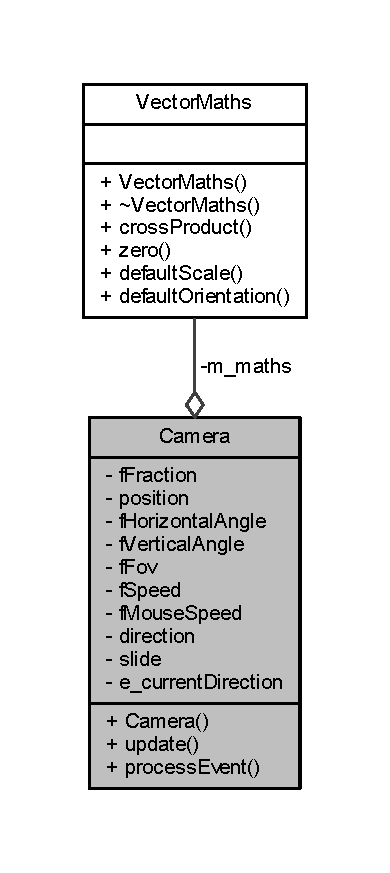
\includegraphics[width=187pt]{class_camera__coll__graph}
\end{center}
\end{figure}
\subsection*{Public Member Functions}
\begin{DoxyCompactItemize}
\item 
\hyperlink{class_camera_a01f94c3543f56ede7af49dc778f19331}{Camera} ()
\item 
void \hyperlink{class_camera_a63a7ff68975d02c10e421439685adff0}{update} (float f\+Elapsed\+Time, sf\+::\+Vector2i i\+Mouse\+Position, int i\+Screen\+Width, int i\+Screen\+Height)
\item 
void \hyperlink{class_camera_a62fb0fe8f7e8ea62124a74cb41416b68}{process\+Event} (sf\+::\+Event \&e)
\end{DoxyCompactItemize}
\subsection*{Private Types}
\begin{DoxyCompactItemize}
\item 
enum \hyperlink{class_camera_a80cb65605322d27ad3b6d973484509ec}{Direction} \{ \\*
\hyperlink{class_camera_a80cb65605322d27ad3b6d973484509ecabbe3f3250295458287d080a1bd22836a}{Up}, 
\hyperlink{class_camera_a80cb65605322d27ad3b6d973484509eca9f55780b3556dc9a198ca80fe11e26fa}{Down}, 
\hyperlink{class_camera_a80cb65605322d27ad3b6d973484509eca078c43b15f9bbb911f662106bbf292a8}{Left}, 
\hyperlink{class_camera_a80cb65605322d27ad3b6d973484509eca75a19c746d87ee2091237f031dd8ad0c}{Right}, 
\\*
\hyperlink{class_camera_a80cb65605322d27ad3b6d973484509ecadaa005f6e4daa20b11e955258d295365}{Fly\+Up}, 
\hyperlink{class_camera_a80cb65605322d27ad3b6d973484509ecae3ff7ee5ba825d57db07cd92e2023a16}{Fly\+Down}, 
\hyperlink{class_camera_a80cb65605322d27ad3b6d973484509ecaada69810ee243aebf719c5b2e9982c11}{None}
 \}
\end{DoxyCompactItemize}
\subsection*{Private Attributes}
\begin{DoxyCompactItemize}
\item 
float \hyperlink{class_camera_a74b69f00fa9be5cfcc62df59fdbb9b8b}{f\+Fraction}
\item 
sf\+::\+Vector3f \hyperlink{class_camera_a7a74f182c7bf64bb7e3238a38a251156}{position}
\item 
float \hyperlink{class_camera_a3a8aadb8799bae49c8ddbe18ffd18844}{f\+Horizontal\+Angle}
\item 
float \hyperlink{class_camera_ada1359a4c866f93aa97fb663db45bb69}{f\+Vertical\+Angle}
\item 
float \hyperlink{class_camera_a8038d7c06da7d521ae843631efb69598}{f\+Fov}
\item 
float \hyperlink{class_camera_aeb8498caa945fa6f40756ef523b2ee14}{f\+Speed}
\item 
float \hyperlink{class_camera_a450d3b9ceabac106ea9703e5b5cd3738}{f\+Mouse\+Speed}
\item 
sf\+::\+Vector3f \hyperlink{class_camera_a97ef59710eec2c701e285d1b8e9d5adf}{direction}
\item 
sf\+::\+Vector3f \hyperlink{class_camera_a0ecb048ae43024cfda52267918e6c87e}{slide}
\item 
\hyperlink{class_camera_a80cb65605322d27ad3b6d973484509ec}{Direction} \hyperlink{class_camera_a39326efe4367d5e4260ae9316240e9b2}{e\+\_\+current\+Direction}
\item 
\hyperlink{class_vector_maths}{Vector\+Maths} \hyperlink{class_camera_a12c980cdff20aedc0f6ac08b985757aa}{m\+\_\+maths}
\end{DoxyCompactItemize}


\subsection{Detailed Description}
This class is used to create a camera. 

\subsection{Member Enumeration Documentation}
\index{Camera@{Camera}!Direction@{Direction}}
\index{Direction@{Direction}!Camera@{Camera}}
\subsubsection[{\texorpdfstring{Direction}{Direction}}]{\setlength{\rightskip}{0pt plus 5cm}enum {\bf Camera\+::\+Direction}\hspace{0.3cm}{\ttfamily [private]}}\hypertarget{class_camera_a80cb65605322d27ad3b6d973484509ec}{}\label{class_camera_a80cb65605322d27ad3b6d973484509ec}
Direction state of a camera. \begin{Desc}
\item[Enumerator]\par
\begin{description}
\index{Up@{Up}!Camera@{Camera}}\index{Camera@{Camera}!Up@{Up}}\item[{\em 
Up\hypertarget{class_camera_a80cb65605322d27ad3b6d973484509ecabbe3f3250295458287d080a1bd22836a}{}\label{class_camera_a80cb65605322d27ad3b6d973484509ecabbe3f3250295458287d080a1bd22836a}
}]We are going up. \index{Down@{Down}!Camera@{Camera}}\index{Camera@{Camera}!Down@{Down}}\item[{\em 
Down\hypertarget{class_camera_a80cb65605322d27ad3b6d973484509eca9f55780b3556dc9a198ca80fe11e26fa}{}\label{class_camera_a80cb65605322d27ad3b6d973484509eca9f55780b3556dc9a198ca80fe11e26fa}
}]We are going down. \index{Left@{Left}!Camera@{Camera}}\index{Camera@{Camera}!Left@{Left}}\item[{\em 
Left\hypertarget{class_camera_a80cb65605322d27ad3b6d973484509eca078c43b15f9bbb911f662106bbf292a8}{}\label{class_camera_a80cb65605322d27ad3b6d973484509eca078c43b15f9bbb911f662106bbf292a8}
}]We are going left. \index{Right@{Right}!Camera@{Camera}}\index{Camera@{Camera}!Right@{Right}}\item[{\em 
Right\hypertarget{class_camera_a80cb65605322d27ad3b6d973484509eca75a19c746d87ee2091237f031dd8ad0c}{}\label{class_camera_a80cb65605322d27ad3b6d973484509eca75a19c746d87ee2091237f031dd8ad0c}
}]We are going right. \index{Fly\+Up@{Fly\+Up}!Camera@{Camera}}\index{Camera@{Camera}!Fly\+Up@{Fly\+Up}}\item[{\em 
Fly\+Up\hypertarget{class_camera_a80cb65605322d27ad3b6d973484509ecadaa005f6e4daa20b11e955258d295365}{}\label{class_camera_a80cb65605322d27ad3b6d973484509ecadaa005f6e4daa20b11e955258d295365}
}]We fly up. \index{Fly\+Down@{Fly\+Down}!Camera@{Camera}}\index{Camera@{Camera}!Fly\+Down@{Fly\+Down}}\item[{\em 
Fly\+Down\hypertarget{class_camera_a80cb65605322d27ad3b6d973484509ecae3ff7ee5ba825d57db07cd92e2023a16}{}\label{class_camera_a80cb65605322d27ad3b6d973484509ecae3ff7ee5ba825d57db07cd92e2023a16}
}]We fly down. \index{None@{None}!Camera@{Camera}}\index{Camera@{Camera}!None@{None}}\item[{\em 
None\hypertarget{class_camera_a80cb65605322d27ad3b6d973484509ecaada69810ee243aebf719c5b2e9982c11}{}\label{class_camera_a80cb65605322d27ad3b6d973484509ecaada69810ee243aebf719c5b2e9982c11}
}]None = We are not moving. \end{description}
\end{Desc}


\subsection{Constructor \& Destructor Documentation}
\index{Camera@{Camera}!Camera@{Camera}}
\index{Camera@{Camera}!Camera@{Camera}}
\subsubsection[{\texorpdfstring{Camera()}{Camera()}}]{\setlength{\rightskip}{0pt plus 5cm}Camera\+::\+Camera (
\begin{DoxyParamCaption}
{}
\end{DoxyParamCaption}
)}\hypertarget{class_camera_a01f94c3543f56ede7af49dc778f19331}{}\label{class_camera_a01f94c3543f56ede7af49dc778f19331}
Constructor. 

\subsection{Member Function Documentation}
\index{Camera@{Camera}!process\+Event@{process\+Event}}
\index{process\+Event@{process\+Event}!Camera@{Camera}}
\subsubsection[{\texorpdfstring{process\+Event(sf\+::\+Event \&e)}{processEvent(sf::Event &e)}}]{\setlength{\rightskip}{0pt plus 5cm}void Camera\+::process\+Event (
\begin{DoxyParamCaption}
\item[{sf\+::\+Event \&}]{e}
\end{DoxyParamCaption}
)}\hypertarget{class_camera_a62fb0fe8f7e8ea62124a74cb41416b68}{}\label{class_camera_a62fb0fe8f7e8ea62124a74cb41416b68}
Process any events. 
\begin{DoxyParams}{Parameters}
{\em e} & = Event to be processed. \\
\hline
\end{DoxyParams}
\index{Camera@{Camera}!update@{update}}
\index{update@{update}!Camera@{Camera}}
\subsubsection[{\texorpdfstring{update(float f\+Elapsed\+Time, sf\+::\+Vector2i i\+Mouse\+Position, int i\+Screen\+Width, int i\+Screen\+Height)}{update(float fElapsedTime, sf::Vector2i iMousePosition, int iScreenWidth, int iScreenHeight)}}]{\setlength{\rightskip}{0pt plus 5cm}void Camera\+::update (
\begin{DoxyParamCaption}
\item[{float}]{f\+Elapsed\+Time, }
\item[{sf\+::\+Vector2i}]{i\+Mouse\+Position, }
\item[{int}]{i\+Screen\+Width, }
\item[{int}]{i\+Screen\+Height}
\end{DoxyParamCaption}
)}\hypertarget{class_camera_a63a7ff68975d02c10e421439685adff0}{}\label{class_camera_a63a7ff68975d02c10e421439685adff0}
Update our camera. 
\begin{DoxyParams}{Parameters}
{\em f\+Elapsed\+Time} & = Refresh rate. \\
\hline
{\em i\+Mouse\+Position} & = Mouse position. \\
\hline
{\em i\+Screen\+Width} & = Screen width. \\
\hline
{\em i\+Screen\+Height} & = Screen height. \\
\hline
\end{DoxyParams}


\subsection{Member Data Documentation}
\index{Camera@{Camera}!direction@{direction}}
\index{direction@{direction}!Camera@{Camera}}
\subsubsection[{\texorpdfstring{direction}{direction}}]{\setlength{\rightskip}{0pt plus 5cm}sf\+::\+Vector3f Camera\+::direction\hspace{0.3cm}{\ttfamily [private]}}\hypertarget{class_camera_a97ef59710eec2c701e285d1b8e9d5adf}{}\label{class_camera_a97ef59710eec2c701e285d1b8e9d5adf}
Direction of a camera. \index{Camera@{Camera}!e\+\_\+current\+Direction@{e\+\_\+current\+Direction}}
\index{e\+\_\+current\+Direction@{e\+\_\+current\+Direction}!Camera@{Camera}}
\subsubsection[{\texorpdfstring{e\+\_\+current\+Direction}{e_currentDirection}}]{\setlength{\rightskip}{0pt plus 5cm}{\bf Direction} Camera\+::e\+\_\+current\+Direction\hspace{0.3cm}{\ttfamily [private]}}\hypertarget{class_camera_a39326efe4367d5e4260ae9316240e9b2}{}\label{class_camera_a39326efe4367d5e4260ae9316240e9b2}
Our current direction. \index{Camera@{Camera}!f\+Fov@{f\+Fov}}
\index{f\+Fov@{f\+Fov}!Camera@{Camera}}
\subsubsection[{\texorpdfstring{f\+Fov}{fFov}}]{\setlength{\rightskip}{0pt plus 5cm}float Camera\+::f\+Fov\hspace{0.3cm}{\ttfamily [private]}}\hypertarget{class_camera_a8038d7c06da7d521ae843631efb69598}{}\label{class_camera_a8038d7c06da7d521ae843631efb69598}
Field of View. \index{Camera@{Camera}!f\+Fraction@{f\+Fraction}}
\index{f\+Fraction@{f\+Fraction}!Camera@{Camera}}
\subsubsection[{\texorpdfstring{f\+Fraction}{fFraction}}]{\setlength{\rightskip}{0pt plus 5cm}float Camera\+::f\+Fraction\hspace{0.3cm}{\ttfamily [private]}}\hypertarget{class_camera_a74b69f00fa9be5cfcc62df59fdbb9b8b}{}\label{class_camera_a74b69f00fa9be5cfcc62df59fdbb9b8b}
The fraction is a possible speed implementation. \index{Camera@{Camera}!f\+Horizontal\+Angle@{f\+Horizontal\+Angle}}
\index{f\+Horizontal\+Angle@{f\+Horizontal\+Angle}!Camera@{Camera}}
\subsubsection[{\texorpdfstring{f\+Horizontal\+Angle}{fHorizontalAngle}}]{\setlength{\rightskip}{0pt plus 5cm}float Camera\+::f\+Horizontal\+Angle\hspace{0.3cm}{\ttfamily [private]}}\hypertarget{class_camera_a3a8aadb8799bae49c8ddbe18ffd18844}{}\label{class_camera_a3a8aadb8799bae49c8ddbe18ffd18844}
Horizontal angle. \index{Camera@{Camera}!f\+Mouse\+Speed@{f\+Mouse\+Speed}}
\index{f\+Mouse\+Speed@{f\+Mouse\+Speed}!Camera@{Camera}}
\subsubsection[{\texorpdfstring{f\+Mouse\+Speed}{fMouseSpeed}}]{\setlength{\rightskip}{0pt plus 5cm}float Camera\+::f\+Mouse\+Speed\hspace{0.3cm}{\ttfamily [private]}}\hypertarget{class_camera_a450d3b9ceabac106ea9703e5b5cd3738}{}\label{class_camera_a450d3b9ceabac106ea9703e5b5cd3738}
Mouse sensitivbity. \index{Camera@{Camera}!f\+Speed@{f\+Speed}}
\index{f\+Speed@{f\+Speed}!Camera@{Camera}}
\subsubsection[{\texorpdfstring{f\+Speed}{fSpeed}}]{\setlength{\rightskip}{0pt plus 5cm}float Camera\+::f\+Speed\hspace{0.3cm}{\ttfamily [private]}}\hypertarget{class_camera_aeb8498caa945fa6f40756ef523b2ee14}{}\label{class_camera_aeb8498caa945fa6f40756ef523b2ee14}
Movement speed of a camera. \index{Camera@{Camera}!f\+Vertical\+Angle@{f\+Vertical\+Angle}}
\index{f\+Vertical\+Angle@{f\+Vertical\+Angle}!Camera@{Camera}}
\subsubsection[{\texorpdfstring{f\+Vertical\+Angle}{fVerticalAngle}}]{\setlength{\rightskip}{0pt plus 5cm}float Camera\+::f\+Vertical\+Angle\hspace{0.3cm}{\ttfamily [private]}}\hypertarget{class_camera_ada1359a4c866f93aa97fb663db45bb69}{}\label{class_camera_ada1359a4c866f93aa97fb663db45bb69}
Vertical angle. \index{Camera@{Camera}!m\+\_\+maths@{m\+\_\+maths}}
\index{m\+\_\+maths@{m\+\_\+maths}!Camera@{Camera}}
\subsubsection[{\texorpdfstring{m\+\_\+maths}{m_maths}}]{\setlength{\rightskip}{0pt plus 5cm}{\bf Vector\+Maths} Camera\+::m\+\_\+maths\hspace{0.3cm}{\ttfamily [private]}}\hypertarget{class_camera_a12c980cdff20aedc0f6ac08b985757aa}{}\label{class_camera_a12c980cdff20aedc0f6ac08b985757aa}
Maths. \index{Camera@{Camera}!position@{position}}
\index{position@{position}!Camera@{Camera}}
\subsubsection[{\texorpdfstring{position}{position}}]{\setlength{\rightskip}{0pt plus 5cm}sf\+::\+Vector3f Camera\+::position\hspace{0.3cm}{\ttfamily [private]}}\hypertarget{class_camera_a7a74f182c7bf64bb7e3238a38a251156}{}\label{class_camera_a7a74f182c7bf64bb7e3238a38a251156}
\hyperlink{class_camera}{Camera} position. \index{Camera@{Camera}!slide@{slide}}
\index{slide@{slide}!Camera@{Camera}}
\subsubsection[{\texorpdfstring{slide}{slide}}]{\setlength{\rightskip}{0pt plus 5cm}sf\+::\+Vector3f Camera\+::slide\hspace{0.3cm}{\ttfamily [private]}}\hypertarget{class_camera_a0ecb048ae43024cfda52267918e6c87e}{}\label{class_camera_a0ecb048ae43024cfda52267918e6c87e}
\hyperlink{class_camera}{Camera} moving to the side. 

The documentation for this class was generated from the following file\+:\begin{DoxyCompactItemize}
\item 
C\+:/\+Airport/include/\hyperlink{camera_8h}{camera.\+h}\end{DoxyCompactItemize}

\hypertarget{class_lighting}{}\section{Lighting Class Reference}
\label{class_lighting}\index{Lighting@{Lighting}}


This class is used to create a lighting.  




{\ttfamily \#include $<$lighting.\+h$>$}



Collaboration diagram for Lighting\+:\nopagebreak
\begin{figure}[H]
\begin{center}
\leavevmode
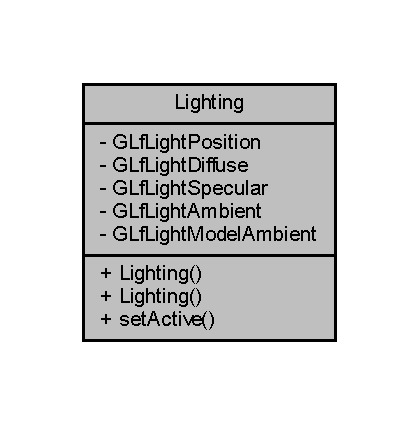
\includegraphics[width=201pt]{class_lighting__coll__graph}
\end{center}
\end{figure}
\subsection*{Public Member Functions}
\begin{DoxyCompactItemize}
\item 
\hyperlink{class_lighting_a0077cde5c3f7a5a4e24617ce784b416f}{Lighting} ()
\item 
\hyperlink{class_lighting_a6f8057acf2f88c348490872d74273891}{Lighting} (sf\+::\+Vector3f position\+In, float f\+PositionW, sf\+::\+Vector3f diffuse, float f\+DiffuseW, sf\+::\+Vector3f specular, float f\+SpecularW, sf\+::\+Vector3f ambient, float f\+AmbientW)
\item 
void \hyperlink{class_lighting_a067ea4fccca5456f08867ae153f1f9a7}{set\+Active} (G\+Lenum i\+Light\+Number, std\+::string s\+Ambient\+Type)
\end{DoxyCompactItemize}
\subsection*{Private Attributes}
\begin{DoxyCompactItemize}
\item 
G\+Lfloat \hyperlink{class_lighting_ac32a0644e1cf1fcbbcfd4cc9fd64dadc}{G\+Lf\+Light\+Position} \mbox{[}4\mbox{]}
\item 
G\+Lfloat \hyperlink{class_lighting_ae01c2bdb028d5fd91669809f274b9d8a}{G\+Lf\+Light\+Diffuse} \mbox{[}4\mbox{]}
\item 
G\+Lfloat \hyperlink{class_lighting_a931695dbe1f392f986a2a47434243f10}{G\+Lf\+Light\+Specular} \mbox{[}4\mbox{]}
\item 
G\+Lfloat \hyperlink{class_lighting_a4d0d2a9b0b16005ce211fc1a3e51f61c}{G\+Lf\+Light\+Ambient} \mbox{[}4\mbox{]}
\item 
G\+Lfloat \hyperlink{class_lighting_adaf2dbed9918074abc9aa6baa0cb2874}{G\+Lf\+Light\+Model\+Ambient} \mbox{[}4\mbox{]}
\end{DoxyCompactItemize}


\subsection{Detailed Description}
This class is used to create a lighting. 

\subsection{Constructor \& Destructor Documentation}
\index{Lighting@{Lighting}!Lighting@{Lighting}}
\index{Lighting@{Lighting}!Lighting@{Lighting}}
\subsubsection[{\texorpdfstring{Lighting()}{Lighting()}}]{\setlength{\rightskip}{0pt plus 5cm}Lighting\+::\+Lighting (
\begin{DoxyParamCaption}
{}
\end{DoxyParamCaption}
)\hspace{0.3cm}{\ttfamily [inline]}}\hypertarget{class_lighting_a0077cde5c3f7a5a4e24617ce784b416f}{}\label{class_lighting_a0077cde5c3f7a5a4e24617ce784b416f}
Constructor. 

Here is the call graph for this function\+:\nopagebreak
\begin{figure}[H]
\begin{center}
\leavevmode
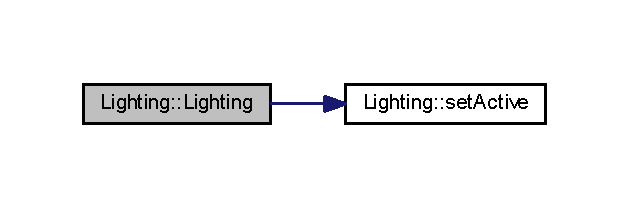
\includegraphics[width=302pt]{class_lighting_a0077cde5c3f7a5a4e24617ce784b416f_cgraph}
\end{center}
\end{figure}


\index{Lighting@{Lighting}!Lighting@{Lighting}}
\index{Lighting@{Lighting}!Lighting@{Lighting}}
\subsubsection[{\texorpdfstring{Lighting(sf\+::\+Vector3f position\+In, float f\+Position\+W, sf\+::\+Vector3f diffuse, float f\+Diffuse\+W, sf\+::\+Vector3f specular, float f\+Specular\+W, sf\+::\+Vector3f ambient, float f\+Ambient\+W)}{Lighting(sf::Vector3f positionIn, float fPositionW, sf::Vector3f diffuse, float fDiffuseW, sf::Vector3f specular, float fSpecularW, sf::Vector3f ambient, float fAmbientW)}}]{\setlength{\rightskip}{0pt plus 5cm}Lighting\+::\+Lighting (
\begin{DoxyParamCaption}
\item[{sf\+::\+Vector3f}]{position\+In, }
\item[{float}]{f\+PositionW, }
\item[{sf\+::\+Vector3f}]{diffuse, }
\item[{float}]{f\+DiffuseW, }
\item[{sf\+::\+Vector3f}]{specular, }
\item[{float}]{f\+SpecularW, }
\item[{sf\+::\+Vector3f}]{ambient, }
\item[{float}]{f\+AmbientW}
\end{DoxyParamCaption}
)}\hypertarget{class_lighting_a6f8057acf2f88c348490872d74273891}{}\label{class_lighting_a6f8057acf2f88c348490872d74273891}
Light initializer. 
\begin{DoxyParams}{Parameters}
{\em position\+In} & = Position of the light. \\
\hline
{\em f\+PositionW} & = 1.\+f for directional, 0.\+f for spot light \\
\hline
{\em diffuse} & = Diffuse effect. \\
\hline
{\em f\+DiffuseW} & = Leave this at 1.\+f!!!. \\
\hline
{\em specular} & = Specular effect. \\
\hline
{\em f\+SpecularW} & = Leave this at 1.\+f!!!. \\
\hline
{\em ambient} & = Ambient effect. \\
\hline
{\em f\+AmbientW} & = Leave this at 1.\+f!!!. \\
\hline
\end{DoxyParams}


\subsection{Member Function Documentation}
\index{Lighting@{Lighting}!set\+Active@{set\+Active}}
\index{set\+Active@{set\+Active}!Lighting@{Lighting}}
\subsubsection[{\texorpdfstring{set\+Active(\+G\+Lenum i\+Light\+Number, std\+::string s\+Ambient\+Type)}{setActive(GLenum iLightNumber, std::string sAmbientType)}}]{\setlength{\rightskip}{0pt plus 5cm}void Lighting\+::set\+Active (
\begin{DoxyParamCaption}
\item[{G\+Lenum}]{i\+Light\+Number, }
\item[{std\+::string}]{s\+Ambient\+Type}
\end{DoxyParamCaption}
)}\hypertarget{class_lighting_a067ea4fccca5456f08867ae153f1f9a7}{}\label{class_lighting_a067ea4fccca5456f08867ae153f1f9a7}
Activate the light source. 
\begin{DoxyParams}{Parameters}
{\em i\+Light\+Number} & = Light number. You can only have maximum of 8 light sources active. \\
\hline
{\em s\+Ambient\+Type} & = Type of an ambient light \\
\hline
\end{DoxyParams}


\subsection{Member Data Documentation}
\index{Lighting@{Lighting}!G\+Lf\+Light\+Ambient@{G\+Lf\+Light\+Ambient}}
\index{G\+Lf\+Light\+Ambient@{G\+Lf\+Light\+Ambient}!Lighting@{Lighting}}
\subsubsection[{\texorpdfstring{G\+Lf\+Light\+Ambient}{GLfLightAmbient}}]{\setlength{\rightskip}{0pt plus 5cm}G\+Lfloat Lighting\+::\+G\+Lf\+Light\+Ambient\mbox{[}4\mbox{]}\hspace{0.3cm}{\ttfamily [private]}}\hypertarget{class_lighting_a4d0d2a9b0b16005ce211fc1a3e51f61c}{}\label{class_lighting_a4d0d2a9b0b16005ce211fc1a3e51f61c}
Ambient light. \index{Lighting@{Lighting}!G\+Lf\+Light\+Diffuse@{G\+Lf\+Light\+Diffuse}}
\index{G\+Lf\+Light\+Diffuse@{G\+Lf\+Light\+Diffuse}!Lighting@{Lighting}}
\subsubsection[{\texorpdfstring{G\+Lf\+Light\+Diffuse}{GLfLightDiffuse}}]{\setlength{\rightskip}{0pt plus 5cm}G\+Lfloat Lighting\+::\+G\+Lf\+Light\+Diffuse\mbox{[}4\mbox{]}\hspace{0.3cm}{\ttfamily [private]}}\hypertarget{class_lighting_ae01c2bdb028d5fd91669809f274b9d8a}{}\label{class_lighting_ae01c2bdb028d5fd91669809f274b9d8a}
Diffuse light. \index{Lighting@{Lighting}!G\+Lf\+Light\+Model\+Ambient@{G\+Lf\+Light\+Model\+Ambient}}
\index{G\+Lf\+Light\+Model\+Ambient@{G\+Lf\+Light\+Model\+Ambient}!Lighting@{Lighting}}
\subsubsection[{\texorpdfstring{G\+Lf\+Light\+Model\+Ambient}{GLfLightModelAmbient}}]{\setlength{\rightskip}{0pt plus 5cm}G\+Lfloat Lighting\+::\+G\+Lf\+Light\+Model\+Ambient\mbox{[}4\mbox{]}\hspace{0.3cm}{\ttfamily [private]}}\hypertarget{class_lighting_adaf2dbed9918074abc9aa6baa0cb2874}{}\label{class_lighting_adaf2dbed9918074abc9aa6baa0cb2874}
\hyperlink{class_model}{Model} ambient light. \index{Lighting@{Lighting}!G\+Lf\+Light\+Position@{G\+Lf\+Light\+Position}}
\index{G\+Lf\+Light\+Position@{G\+Lf\+Light\+Position}!Lighting@{Lighting}}
\subsubsection[{\texorpdfstring{G\+Lf\+Light\+Position}{GLfLightPosition}}]{\setlength{\rightskip}{0pt plus 5cm}G\+Lfloat Lighting\+::\+G\+Lf\+Light\+Position\mbox{[}4\mbox{]}\hspace{0.3cm}{\ttfamily [private]}}\hypertarget{class_lighting_ac32a0644e1cf1fcbbcfd4cc9fd64dadc}{}\label{class_lighting_ac32a0644e1cf1fcbbcfd4cc9fd64dadc}
Light position. \index{Lighting@{Lighting}!G\+Lf\+Light\+Specular@{G\+Lf\+Light\+Specular}}
\index{G\+Lf\+Light\+Specular@{G\+Lf\+Light\+Specular}!Lighting@{Lighting}}
\subsubsection[{\texorpdfstring{G\+Lf\+Light\+Specular}{GLfLightSpecular}}]{\setlength{\rightskip}{0pt plus 5cm}G\+Lfloat Lighting\+::\+G\+Lf\+Light\+Specular\mbox{[}4\mbox{]}\hspace{0.3cm}{\ttfamily [private]}}\hypertarget{class_lighting_a931695dbe1f392f986a2a47434243f10}{}\label{class_lighting_a931695dbe1f392f986a2a47434243f10}
Specular light. 

The documentation for this class was generated from the following file\+:\begin{DoxyCompactItemize}
\item 
C\+:/\+Airport/include/\hyperlink{lighting_8h}{lighting.\+h}\end{DoxyCompactItemize}

\hypertarget{class_material}{}\section{Material Class Reference}
\label{class_material}\index{Material@{Material}}


This class is used to create a material.  




{\ttfamily \#include $<$material.\+h$>$}



Collaboration diagram for Material\+:\nopagebreak
\begin{figure}[H]
\begin{center}
\leavevmode
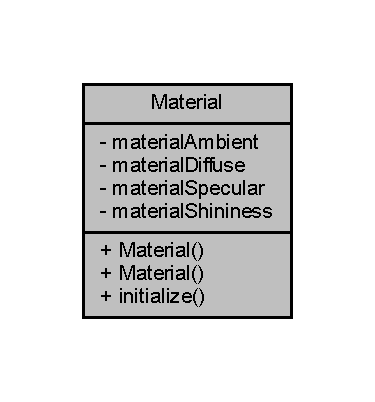
\includegraphics[width=180pt]{class_material__coll__graph}
\end{center}
\end{figure}
\subsection*{Public Member Functions}
\begin{DoxyCompactItemize}
\item 
\hyperlink{class_material_a137e987401b63eb7c6c27c3e38bc74b5}{Material} ()
\item 
\hyperlink{class_material_a37d1580c7ab5e7e31e7210a374d82364}{Material} (sf\+::\+Vector3f ambient, float f\+AmbientW, sf\+::\+Vector3f diffuse, float f\+DiffuseW, sf\+::\+Vector3f specular, float f\+SpecularW, float f\+Shininess)
\item 
void \hyperlink{class_material_aae516fe81f34adfead3ff7ae0cc9c92e}{initialize} (G\+Lenum model\+IN)
\end{DoxyCompactItemize}
\subsection*{Private Attributes}
\begin{DoxyCompactItemize}
\item 
G\+Lfloat \hyperlink{class_material_a2b228dd08317eb9a6f794db264b0a86c}{material\+Ambient} \mbox{[}4\mbox{]}
\item 
G\+Lfloat \hyperlink{class_material_a72c13fb8c76910a05fe13257d96391e6}{material\+Diffuse} \mbox{[}4\mbox{]}
\item 
G\+Lfloat \hyperlink{class_material_ad3daaf8271e92ef553f08edf0878f725}{material\+Specular} \mbox{[}4\mbox{]}
\item 
G\+Lfloat \hyperlink{class_material_aeb155ecd278b3ea891077ff8aea8cd93}{material\+Shininess}
\end{DoxyCompactItemize}


\subsection{Detailed Description}
This class is used to create a material. 

\subsection{Constructor \& Destructor Documentation}
\index{Material@{Material}!Material@{Material}}
\index{Material@{Material}!Material@{Material}}
\subsubsection[{\texorpdfstring{Material()}{Material()}}]{\setlength{\rightskip}{0pt plus 5cm}Material\+::\+Material (
\begin{DoxyParamCaption}
{}
\end{DoxyParamCaption}
)\hspace{0.3cm}{\ttfamily [inline]}}\hypertarget{class_material_a137e987401b63eb7c6c27c3e38bc74b5}{}\label{class_material_a137e987401b63eb7c6c27c3e38bc74b5}
Constructor. 

Here is the call graph for this function\+:\nopagebreak
\begin{figure}[H]
\begin{center}
\leavevmode
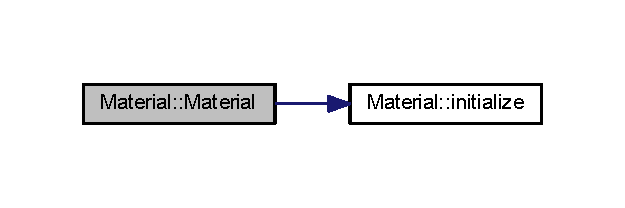
\includegraphics[width=300pt]{class_material_a137e987401b63eb7c6c27c3e38bc74b5_cgraph}
\end{center}
\end{figure}


\index{Material@{Material}!Material@{Material}}
\index{Material@{Material}!Material@{Material}}
\subsubsection[{\texorpdfstring{Material(sf\+::\+Vector3f ambient, float f\+Ambient\+W, sf\+::\+Vector3f diffuse, float f\+Diffuse\+W, sf\+::\+Vector3f specular, float f\+Specular\+W, float f\+Shininess)}{Material(sf::Vector3f ambient, float fAmbientW, sf::Vector3f diffuse, float fDiffuseW, sf::Vector3f specular, float fSpecularW, float fShininess)}}]{\setlength{\rightskip}{0pt plus 5cm}Material\+::\+Material (
\begin{DoxyParamCaption}
\item[{sf\+::\+Vector3f}]{ambient, }
\item[{float}]{f\+AmbientW, }
\item[{sf\+::\+Vector3f}]{diffuse, }
\item[{float}]{f\+DiffuseW, }
\item[{sf\+::\+Vector3f}]{specular, }
\item[{float}]{f\+SpecularW, }
\item[{float}]{f\+Shininess}
\end{DoxyParamCaption}
)}\hypertarget{class_material_a37d1580c7ab5e7e31e7210a374d82364}{}\label{class_material_a37d1580c7ab5e7e31e7210a374d82364}
\hyperlink{class_material}{Material} initializer. 
\begin{DoxyParams}{Parameters}
{\em ambient} & = Ambient effect. \\
\hline
{\em f\+AmbientW} & = Leave this at 1.\+f!!!. \\
\hline
{\em diffuse} & = Diffuse effect. \\
\hline
{\em f\+DiffuseW} & = Leave this at 1.\+f!!!. \\
\hline
{\em specular} & = Specular effect. \\
\hline
{\em f\+SpecularW} & = Leave this at 1.\+f!!!. \\
\hline
{\em f\+Shininess} & = Shniy effect. \\
\hline
\end{DoxyParams}


\subsection{Member Function Documentation}
\index{Material@{Material}!initialize@{initialize}}
\index{initialize@{initialize}!Material@{Material}}
\subsubsection[{\texorpdfstring{initialize(\+G\+Lenum model\+I\+N)}{initialize(GLenum modelIN)}}]{\setlength{\rightskip}{0pt plus 5cm}void Material\+::initialize (
\begin{DoxyParamCaption}
\item[{G\+Lenum}]{model\+IN}
\end{DoxyParamCaption}
)}\hypertarget{class_material_aae516fe81f34adfead3ff7ae0cc9c92e}{}\label{class_material_aae516fe81f34adfead3ff7ae0cc9c92e}
Activates the material for the particular model. 
\begin{DoxyParams}{Parameters}
{\em model\+IN} & = Specific model. \\
\hline
\end{DoxyParams}


\subsection{Member Data Documentation}
\index{Material@{Material}!material\+Ambient@{material\+Ambient}}
\index{material\+Ambient@{material\+Ambient}!Material@{Material}}
\subsubsection[{\texorpdfstring{material\+Ambient}{materialAmbient}}]{\setlength{\rightskip}{0pt plus 5cm}G\+Lfloat Material\+::material\+Ambient\mbox{[}4\mbox{]}\hspace{0.3cm}{\ttfamily [private]}}\hypertarget{class_material_a2b228dd08317eb9a6f794db264b0a86c}{}\label{class_material_a2b228dd08317eb9a6f794db264b0a86c}
\hyperlink{class_material}{Material} ambient effect. \index{Material@{Material}!material\+Diffuse@{material\+Diffuse}}
\index{material\+Diffuse@{material\+Diffuse}!Material@{Material}}
\subsubsection[{\texorpdfstring{material\+Diffuse}{materialDiffuse}}]{\setlength{\rightskip}{0pt plus 5cm}G\+Lfloat Material\+::material\+Diffuse\mbox{[}4\mbox{]}\hspace{0.3cm}{\ttfamily [private]}}\hypertarget{class_material_a72c13fb8c76910a05fe13257d96391e6}{}\label{class_material_a72c13fb8c76910a05fe13257d96391e6}
\hyperlink{class_material}{Material} diffuse effect. \index{Material@{Material}!material\+Shininess@{material\+Shininess}}
\index{material\+Shininess@{material\+Shininess}!Material@{Material}}
\subsubsection[{\texorpdfstring{material\+Shininess}{materialShininess}}]{\setlength{\rightskip}{0pt plus 5cm}G\+Lfloat Material\+::material\+Shininess\hspace{0.3cm}{\ttfamily [private]}}\hypertarget{class_material_aeb155ecd278b3ea891077ff8aea8cd93}{}\label{class_material_aeb155ecd278b3ea891077ff8aea8cd93}
\hyperlink{class_material}{Material} shininess effect. \index{Material@{Material}!material\+Specular@{material\+Specular}}
\index{material\+Specular@{material\+Specular}!Material@{Material}}
\subsubsection[{\texorpdfstring{material\+Specular}{materialSpecular}}]{\setlength{\rightskip}{0pt plus 5cm}G\+Lfloat Material\+::material\+Specular\mbox{[}4\mbox{]}\hspace{0.3cm}{\ttfamily [private]}}\hypertarget{class_material_ad3daaf8271e92ef553f08edf0878f725}{}\label{class_material_ad3daaf8271e92ef553f08edf0878f725}
\hyperlink{class_material}{Material} specular effect. 

The documentation for this class was generated from the following file\+:\begin{DoxyCompactItemize}
\item 
C\+:/\+Airport/include/\hyperlink{material_8h}{material.\+h}\end{DoxyCompactItemize}

\hypertarget{class_model}{}\section{Model Class Reference}
\label{class_model}\index{Model@{Model}}


This class is used to create a model.  




{\ttfamily \#include $<$model.\+h$>$}



Collaboration diagram for Model\+:\nopagebreak
\begin{figure}[H]
\begin{center}
\leavevmode
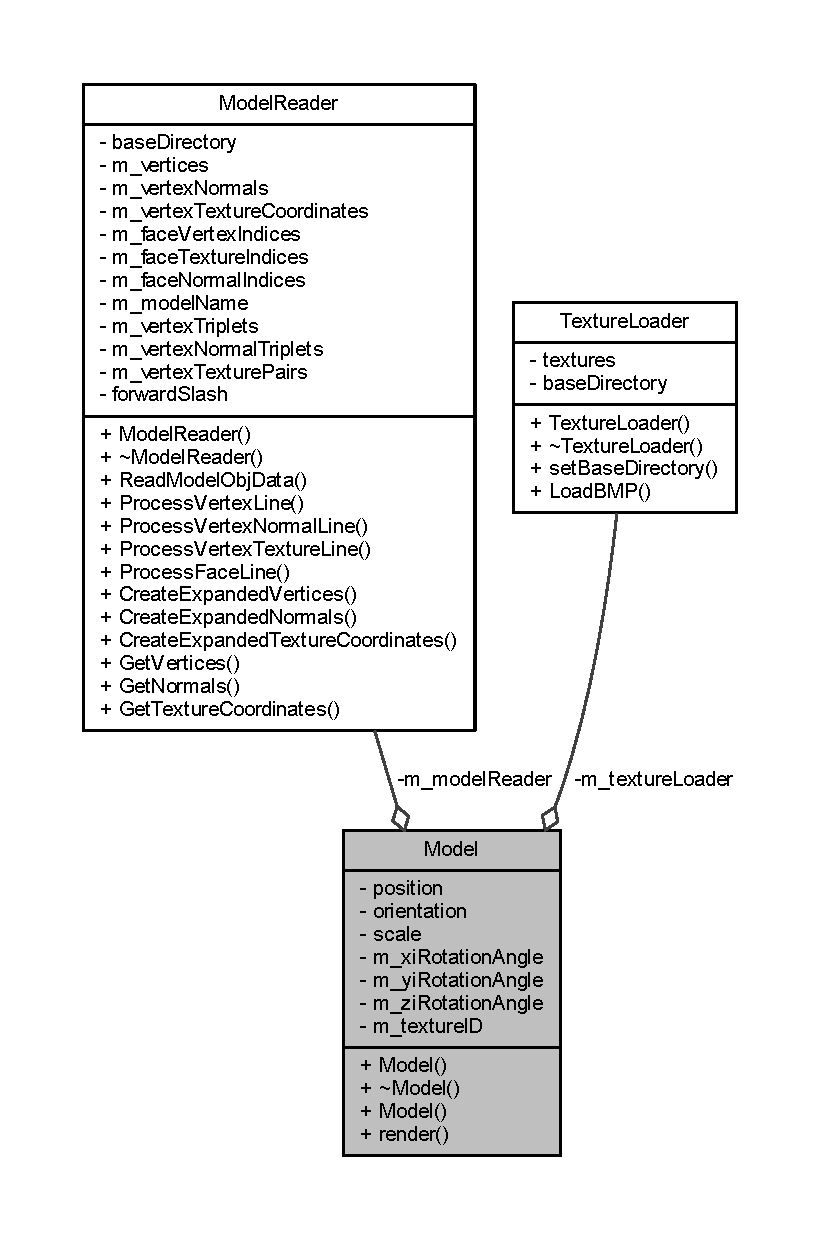
\includegraphics[width=350pt]{class_model__coll__graph}
\end{center}
\end{figure}
\subsection*{Public Member Functions}
\begin{DoxyCompactItemize}
\item 
\hyperlink{class_model_ae3b375de5f6df4faf74a95d64748e048}{Model} ()
\item 
\hyperlink{class_model_ad6ebd2062a0b823db841a0b88baac4c0}{$\sim$\+Model} ()
\item 
\hyperlink{class_model_a76f8ab6b607136cf845617d0c02d4ce9}{Model} (std\+::string s\+File\+Name, std\+::string s\+Texture\+Name, sf\+::\+Vector3f position\+IN, sf\+::\+Vector3f orientation\+IN, sf\+::\+Vector3f scale\+IN)
\item 
void \hyperlink{class_model_a4be6c139cfb3b8bc2903cd536f3b16fb}{render} (bool draw\+With\+Normals, bool draw\+With\+Texture)
\end{DoxyCompactItemize}
\subsection*{Private Attributes}
\begin{DoxyCompactItemize}
\item 
sf\+::\+Vector3f \hyperlink{class_model_a2f25a152b6212faf7d23e6d6ab103d61}{position}
\item 
sf\+::\+Vector3f \hyperlink{class_model_a94eb6111227ec3db203681abd21ebeca}{orientation}
\item 
sf\+::\+Vector3f \hyperlink{class_model_aac1cda61a954d28aa2ee94a1b23de4a9}{scale}
\item 
G\+Luint \hyperlink{class_model_ac0b7f3944641754dba82add1bc4604fc}{m\+\_\+xi\+Rotation\+Angle}
\item 
G\+Luint \hyperlink{class_model_aacf906903bfaa80cb02c46a299016f5e}{m\+\_\+yi\+Rotation\+Angle}
\item 
G\+Luint \hyperlink{class_model_a70be5d2acec40543ec2b9186dfc7cb43}{m\+\_\+zi\+Rotation\+Angle}
\item 
G\+Luint \hyperlink{class_model_a23d182da28544aa34e44752eabaa0422}{m\+\_\+texture\+ID} \mbox{[}2\mbox{]}
\item 
\hyperlink{class_model_reader}{Model\+Reader} $\ast$ \hyperlink{class_model_a3247a4733aa6155e6ed8649cca51d658}{m\+\_\+model\+Reader}
\item 
\hyperlink{class_texture_loader}{Texture\+Loader} $\ast$ \hyperlink{class_model_aade88da2d54d5fa74bd941a1b6f92cc3}{m\+\_\+texture\+Loader}
\end{DoxyCompactItemize}


\subsection{Detailed Description}
This class is used to create a model. 

\subsection{Constructor \& Destructor Documentation}
\index{Model@{Model}!Model@{Model}}
\index{Model@{Model}!Model@{Model}}
\subsubsection[{\texorpdfstring{Model()}{Model()}}]{\setlength{\rightskip}{0pt plus 5cm}Model\+::\+Model (
\begin{DoxyParamCaption}
{}
\end{DoxyParamCaption}
)\hspace{0.3cm}{\ttfamily [inline]}}\hypertarget{class_model_ae3b375de5f6df4faf74a95d64748e048}{}\label{class_model_ae3b375de5f6df4faf74a95d64748e048}
Constructor. \index{Model@{Model}!````~Model@{$\sim$\+Model}}
\index{````~Model@{$\sim$\+Model}!Model@{Model}}
\subsubsection[{\texorpdfstring{$\sim$\+Model()}{~Model()}}]{\setlength{\rightskip}{0pt plus 5cm}Model\+::$\sim$\+Model (
\begin{DoxyParamCaption}
{}
\end{DoxyParamCaption}
)\hspace{0.3cm}{\ttfamily [inline]}}\hypertarget{class_model_ad6ebd2062a0b823db841a0b88baac4c0}{}\label{class_model_ad6ebd2062a0b823db841a0b88baac4c0}
Destructor. 

Here is the call graph for this function\+:\nopagebreak
\begin{figure}[H]
\begin{center}
\leavevmode
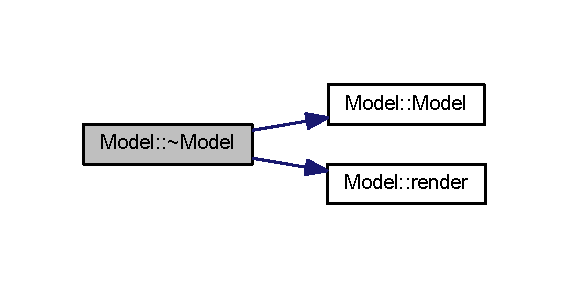
\includegraphics[width=273pt]{class_model_ad6ebd2062a0b823db841a0b88baac4c0_cgraph}
\end{center}
\end{figure}


\index{Model@{Model}!Model@{Model}}
\index{Model@{Model}!Model@{Model}}
\subsubsection[{\texorpdfstring{Model(std\+::string s\+File\+Name, std\+::string s\+Texture\+Name, sf\+::\+Vector3f position\+I\+N, sf\+::\+Vector3f orientation\+I\+N, sf\+::\+Vector3f scale\+I\+N)}{Model(std::string sFileName, std::string sTextureName, sf::Vector3f positionIN, sf::Vector3f orientationIN, sf::Vector3f scaleIN)}}]{\setlength{\rightskip}{0pt plus 5cm}Model\+::\+Model (
\begin{DoxyParamCaption}
\item[{std\+::string}]{s\+File\+Name, }
\item[{std\+::string}]{s\+Texture\+Name, }
\item[{sf\+::\+Vector3f}]{position\+IN, }
\item[{sf\+::\+Vector3f}]{orientation\+IN, }
\item[{sf\+::\+Vector3f}]{scale\+IN}
\end{DoxyParamCaption}
)}\hypertarget{class_model_a76f8ab6b607136cf845617d0c02d4ce9}{}\label{class_model_a76f8ab6b607136cf845617d0c02d4ce9}
\hyperlink{class_model}{Model} constructor. 
\begin{DoxyParams}{Parameters}
{\em s\+File\+Name} & = Name of a file. \\
\hline
{\em s\+Texture\+Name} & = Texture name. \\
\hline
{\em postion\+IN} & = Position of a model. \\
\hline
{\em orientation\+IN} & = Orientation of a model. \\
\hline
{\em scale\+IN} & = Scale of a model. \\
\hline
\end{DoxyParams}


\subsection{Member Function Documentation}
\index{Model@{Model}!render@{render}}
\index{render@{render}!Model@{Model}}
\subsubsection[{\texorpdfstring{render(bool draw\+With\+Normals, bool draw\+With\+Texture)}{render(bool drawWithNormals, bool drawWithTexture)}}]{\setlength{\rightskip}{0pt plus 5cm}void Model\+::render (
\begin{DoxyParamCaption}
\item[{bool}]{draw\+With\+Normals, }
\item[{bool}]{draw\+With\+Texture}
\end{DoxyParamCaption}
)}\hypertarget{class_model_a4be6c139cfb3b8bc2903cd536f3b16fb}{}\label{class_model_a4be6c139cfb3b8bc2903cd536f3b16fb}
\hyperlink{class_model}{Model} rendering. 
\begin{DoxyParams}{Parameters}
{\em draw\+With\+Normals} & = Whether or not to draw with normals. param draw\+With\+Texture = Whether or not to draw with textures. \\
\hline
\end{DoxyParams}


\subsection{Member Data Documentation}
\index{Model@{Model}!m\+\_\+model\+Reader@{m\+\_\+model\+Reader}}
\index{m\+\_\+model\+Reader@{m\+\_\+model\+Reader}!Model@{Model}}
\subsubsection[{\texorpdfstring{m\+\_\+model\+Reader}{m_modelReader}}]{\setlength{\rightskip}{0pt plus 5cm}{\bf Model\+Reader}$\ast$ Model\+::m\+\_\+model\+Reader\hspace{0.3cm}{\ttfamily [private]}}\hypertarget{class_model_a3247a4733aa6155e6ed8649cca51d658}{}\label{class_model_a3247a4733aa6155e6ed8649cca51d658}
\hyperlink{class_model}{Model} reader. \index{Model@{Model}!m\+\_\+texture\+ID@{m\+\_\+texture\+ID}}
\index{m\+\_\+texture\+ID@{m\+\_\+texture\+ID}!Model@{Model}}
\subsubsection[{\texorpdfstring{m\+\_\+texture\+ID}{m_textureID}}]{\setlength{\rightskip}{0pt plus 5cm}G\+Luint Model\+::m\+\_\+texture\+ID\mbox{[}2\mbox{]}\hspace{0.3cm}{\ttfamily [private]}}\hypertarget{class_model_a23d182da28544aa34e44752eabaa0422}{}\label{class_model_a23d182da28544aa34e44752eabaa0422}
A buffer of texture. \index{Model@{Model}!m\+\_\+texture\+Loader@{m\+\_\+texture\+Loader}}
\index{m\+\_\+texture\+Loader@{m\+\_\+texture\+Loader}!Model@{Model}}
\subsubsection[{\texorpdfstring{m\+\_\+texture\+Loader}{m_textureLoader}}]{\setlength{\rightskip}{0pt plus 5cm}{\bf Texture\+Loader}$\ast$ Model\+::m\+\_\+texture\+Loader\hspace{0.3cm}{\ttfamily [private]}}\hypertarget{class_model_aade88da2d54d5fa74bd941a1b6f92cc3}{}\label{class_model_aade88da2d54d5fa74bd941a1b6f92cc3}
Texture loader. \index{Model@{Model}!m\+\_\+xi\+Rotation\+Angle@{m\+\_\+xi\+Rotation\+Angle}}
\index{m\+\_\+xi\+Rotation\+Angle@{m\+\_\+xi\+Rotation\+Angle}!Model@{Model}}
\subsubsection[{\texorpdfstring{m\+\_\+xi\+Rotation\+Angle}{m_xiRotationAngle}}]{\setlength{\rightskip}{0pt plus 5cm}G\+Luint Model\+::m\+\_\+xi\+Rotation\+Angle\hspace{0.3cm}{\ttfamily [private]}}\hypertarget{class_model_ac0b7f3944641754dba82add1bc4604fc}{}\label{class_model_ac0b7f3944641754dba82add1bc4604fc}
Rotation in X axis. \index{Model@{Model}!m\+\_\+yi\+Rotation\+Angle@{m\+\_\+yi\+Rotation\+Angle}}
\index{m\+\_\+yi\+Rotation\+Angle@{m\+\_\+yi\+Rotation\+Angle}!Model@{Model}}
\subsubsection[{\texorpdfstring{m\+\_\+yi\+Rotation\+Angle}{m_yiRotationAngle}}]{\setlength{\rightskip}{0pt plus 5cm}G\+Luint Model\+::m\+\_\+yi\+Rotation\+Angle\hspace{0.3cm}{\ttfamily [private]}}\hypertarget{class_model_aacf906903bfaa80cb02c46a299016f5e}{}\label{class_model_aacf906903bfaa80cb02c46a299016f5e}
Rotation in Y axis. \index{Model@{Model}!m\+\_\+zi\+Rotation\+Angle@{m\+\_\+zi\+Rotation\+Angle}}
\index{m\+\_\+zi\+Rotation\+Angle@{m\+\_\+zi\+Rotation\+Angle}!Model@{Model}}
\subsubsection[{\texorpdfstring{m\+\_\+zi\+Rotation\+Angle}{m_ziRotationAngle}}]{\setlength{\rightskip}{0pt plus 5cm}G\+Luint Model\+::m\+\_\+zi\+Rotation\+Angle\hspace{0.3cm}{\ttfamily [private]}}\hypertarget{class_model_a70be5d2acec40543ec2b9186dfc7cb43}{}\label{class_model_a70be5d2acec40543ec2b9186dfc7cb43}
Rotation in Z axis. \index{Model@{Model}!orientation@{orientation}}
\index{orientation@{orientation}!Model@{Model}}
\subsubsection[{\texorpdfstring{orientation}{orientation}}]{\setlength{\rightskip}{0pt plus 5cm}sf\+::\+Vector3f Model\+::orientation\hspace{0.3cm}{\ttfamily [private]}}\hypertarget{class_model_a94eb6111227ec3db203681abd21ebeca}{}\label{class_model_a94eb6111227ec3db203681abd21ebeca}
Orientation of the model. \index{Model@{Model}!position@{position}}
\index{position@{position}!Model@{Model}}
\subsubsection[{\texorpdfstring{position}{position}}]{\setlength{\rightskip}{0pt plus 5cm}sf\+::\+Vector3f Model\+::position\hspace{0.3cm}{\ttfamily [private]}}\hypertarget{class_model_a2f25a152b6212faf7d23e6d6ab103d61}{}\label{class_model_a2f25a152b6212faf7d23e6d6ab103d61}
Position of the model. \index{Model@{Model}!scale@{scale}}
\index{scale@{scale}!Model@{Model}}
\subsubsection[{\texorpdfstring{scale}{scale}}]{\setlength{\rightskip}{0pt plus 5cm}sf\+::\+Vector3f Model\+::scale\hspace{0.3cm}{\ttfamily [private]}}\hypertarget{class_model_aac1cda61a954d28aa2ee94a1b23de4a9}{}\label{class_model_aac1cda61a954d28aa2ee94a1b23de4a9}
Scale of the model. 

The documentation for this class was generated from the following file\+:\begin{DoxyCompactItemize}
\item 
C\+:/\+Airport/include/\hyperlink{model_8h}{model.\+h}\end{DoxyCompactItemize}

\hypertarget{class_model_extractor}{}\section{Model\+Extractor Class Reference}
\label{class_model_extractor}\index{Model\+Extractor@{Model\+Extractor}}


This class is used to extract information about the model from a file.  




{\ttfamily \#include $<$model\+Extractor.\+h$>$}



Collaboration diagram for Model\+Extractor\+:\nopagebreak
\begin{figure}[H]
\begin{center}
\leavevmode
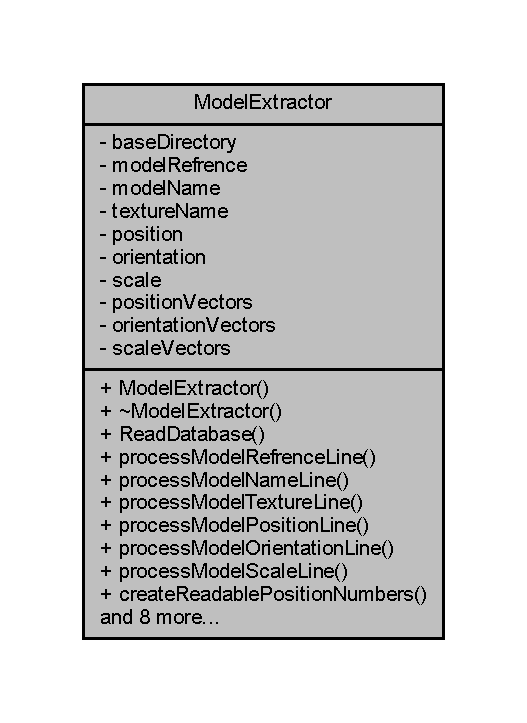
\includegraphics[width=253pt]{class_model_extractor__coll__graph}
\end{center}
\end{figure}
\subsection*{Public Member Functions}
\begin{DoxyCompactItemize}
\item 
\hyperlink{class_model_extractor_a2347486e0a52e3458e9f3e65a120dec2}{Model\+Extractor} (std\+::string file\+Name)
\item 
\hyperlink{class_model_extractor_ab5ad796ee0213f2229bf2f5c6c8eb482}{$\sim$\+Model\+Extractor} ()
\item 
void \hyperlink{class_model_extractor_ab09dc19b136bd09661a4d7ff28fb03a7}{Read\+Database} (std\+::string s\+File\+Name)
\item 
void \hyperlink{class_model_extractor_a7eb2f5737963281bea5ed6ac5de072b0}{process\+Model\+Refrence\+Line} (std\+::istringstream \&iss)
\item 
void \hyperlink{class_model_extractor_af4c4726e7e474552958b4cb2b1f4142e}{process\+Model\+Name\+Line} (std\+::istringstream \&iss)
\item 
void \hyperlink{class_model_extractor_afe64d388bf8efc623af9570303b09ae0}{process\+Model\+Texture\+Line} (std\+::istringstream \&iss)
\item 
void \hyperlink{class_model_extractor_a75c1ea311dfa437712af661cb4943fb3}{process\+Model\+Position\+Line} (std\+::istringstream \&iss)
\item 
void \hyperlink{class_model_extractor_aa437809f62dc7a02b6fe843269d3b342}{process\+Model\+Orientation\+Line} (std\+::istringstream \&iss)
\item 
void \hyperlink{class_model_extractor_a7e66f0061b47a35d6708ee6b8092933c}{process\+Model\+Scale\+Line} (std\+::istringstream \&iss)
\item 
void \hyperlink{class_model_extractor_a0bdda45adf49226dec679b7e3c736478}{create\+Readable\+Position\+Numbers} ()
\item 
void \hyperlink{class_model_extractor_a5dec1fc4b5efefb78ceaec2d603b2081}{create\+Readable\+Orientation\+Numbers} ()
\item 
void \hyperlink{class_model_extractor_a55c88ca5985765592790a0b584426bd2}{create\+Readable\+Scale\+Numbers} ()
\item 
std\+::vector$<$ int $>$ \hyperlink{class_model_extractor_a705e7ffe3d8888c316f35431cb6c58a9}{get\+Refrence} ()
\item 
std\+::vector$<$ std\+::string $>$ \hyperlink{class_model_extractor_a1836d8eebb18bb6bcace2616e0aeb74f}{get\+Name} ()
\item 
std\+::vector$<$ std\+::string $>$ \hyperlink{class_model_extractor_ac925f4f4c80ec4739dcc2c306225519d}{get\+Texture} ()
\item 
std\+::vector$<$ sf\+::\+Vector3f $>$ \hyperlink{class_model_extractor_a9aef3acf4ca5d554649be296044b0c0d}{get\+Position} ()
\item 
std\+::vector$<$ sf\+::\+Vector3f $>$ \hyperlink{class_model_extractor_a2637fe0e4052ff38031a81dd2f00d1b9}{get\+Orientation} ()
\item 
std\+::vector$<$ sf\+::\+Vector3f $>$ \hyperlink{class_model_extractor_a5536264c569072b1cf854e092fd24f02}{get\+Scale} ()
\end{DoxyCompactItemize}
\subsection*{Private Attributes}
\begin{DoxyCompactItemize}
\item 
std\+::string \hyperlink{class_model_extractor_a97d4cac0fe91a0bb91a736f780c8740a}{base\+Directory}
\item 
std\+::vector$<$ int $>$ \hyperlink{class_model_extractor_a507d1a9066e1a5eca6ccabad7a678432}{model\+Refrence}
\item 
std\+::vector$<$ std\+::string $>$ \hyperlink{class_model_extractor_a0167c9a9eab2cd5478f4399a55328db6}{model\+Name}
\item 
std\+::vector$<$ std\+::string $>$ \hyperlink{class_model_extractor_ab1c441c2915f84360bc00b331b301eb2}{texture\+Name}
\item 
std\+::vector$<$ float $>$ \hyperlink{class_model_extractor_a561a692a6b37b8ef36020b918a63066c}{position}
\item 
std\+::vector$<$ float $>$ \hyperlink{class_model_extractor_ae0be066e55d4910fa79d7b3da45100d0}{orientation}
\item 
std\+::vector$<$ float $>$ \hyperlink{class_model_extractor_ae9815e4d0f6783e6ba92961956c7d932}{scale}
\item 
std\+::vector$<$ sf\+::\+Vector3f $>$ \hyperlink{class_model_extractor_a9427f6c960e71ea44371014aa12835cf}{position\+Vectors}
\item 
std\+::vector$<$ sf\+::\+Vector3f $>$ \hyperlink{class_model_extractor_a619bae88ba670b8652dc608a482b23fc}{orientation\+Vectors}
\item 
std\+::vector$<$ sf\+::\+Vector3f $>$ \hyperlink{class_model_extractor_a03bcd2b8bcfffe704b07583ee597b65e}{scale\+Vectors}
\end{DoxyCompactItemize}


\subsection{Detailed Description}
This class is used to extract information about the model from a file. 

\subsection{Constructor \& Destructor Documentation}
\index{Model\+Extractor@{Model\+Extractor}!Model\+Extractor@{Model\+Extractor}}
\index{Model\+Extractor@{Model\+Extractor}!Model\+Extractor@{Model\+Extractor}}
\subsubsection[{\texorpdfstring{Model\+Extractor(std\+::string file\+Name)}{ModelExtractor(std::string fileName)}}]{\setlength{\rightskip}{0pt plus 5cm}Model\+Extractor\+::\+Model\+Extractor (
\begin{DoxyParamCaption}
\item[{std\+::string}]{file\+Name}
\end{DoxyParamCaption}
)}\hypertarget{class_model_extractor_a2347486e0a52e3458e9f3e65a120dec2}{}\label{class_model_extractor_a2347486e0a52e3458e9f3e65a120dec2}
Constructor. 
\begin{DoxyParams}{Parameters}
{\em file\+Name} & = Name of a file. \\
\hline
\end{DoxyParams}
\index{Model\+Extractor@{Model\+Extractor}!````~Model\+Extractor@{$\sim$\+Model\+Extractor}}
\index{````~Model\+Extractor@{$\sim$\+Model\+Extractor}!Model\+Extractor@{Model\+Extractor}}
\subsubsection[{\texorpdfstring{$\sim$\+Model\+Extractor()}{~ModelExtractor()}}]{\setlength{\rightskip}{0pt plus 5cm}Model\+Extractor\+::$\sim$\+Model\+Extractor (
\begin{DoxyParamCaption}
{}
\end{DoxyParamCaption}
)\hspace{0.3cm}{\ttfamily [inline]}}\hypertarget{class_model_extractor_ab5ad796ee0213f2229bf2f5c6c8eb482}{}\label{class_model_extractor_ab5ad796ee0213f2229bf2f5c6c8eb482}
Desctructor. 

Here is the call graph for this function\+:\nopagebreak
\begin{figure}[H]
\begin{center}
\leavevmode
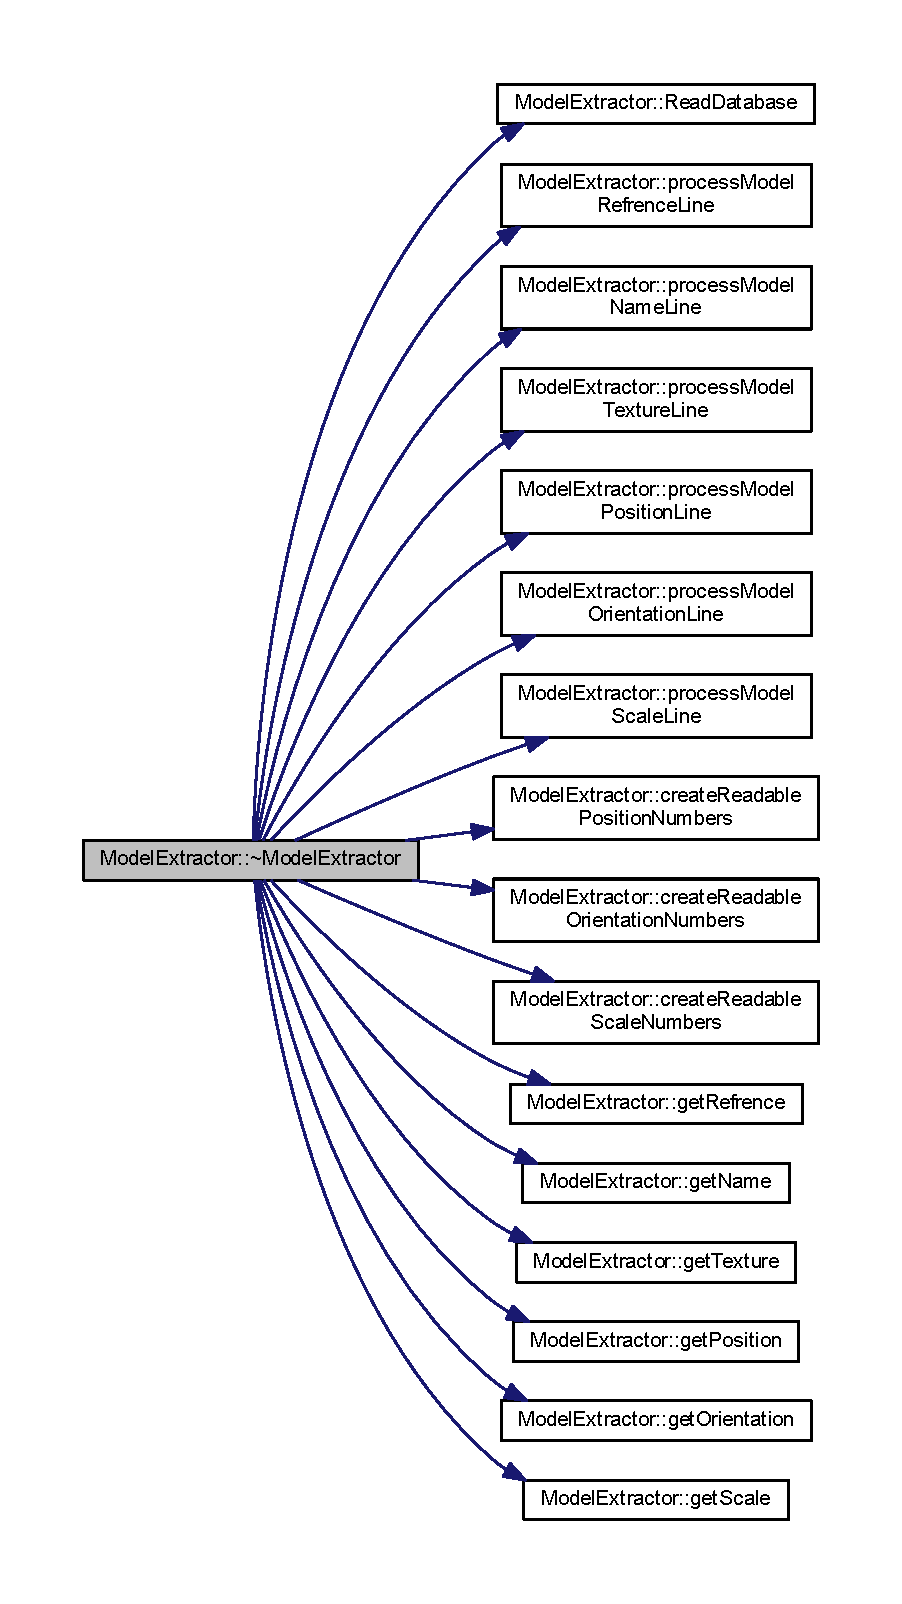
\includegraphics[height=550pt]{class_model_extractor_ab5ad796ee0213f2229bf2f5c6c8eb482_cgraph}
\end{center}
\end{figure}




\subsection{Member Function Documentation}
\index{Model\+Extractor@{Model\+Extractor}!create\+Readable\+Orientation\+Numbers@{create\+Readable\+Orientation\+Numbers}}
\index{create\+Readable\+Orientation\+Numbers@{create\+Readable\+Orientation\+Numbers}!Model\+Extractor@{Model\+Extractor}}
\subsubsection[{\texorpdfstring{create\+Readable\+Orientation\+Numbers()}{createReadableOrientationNumbers()}}]{\setlength{\rightskip}{0pt plus 5cm}void Model\+Extractor\+::create\+Readable\+Orientation\+Numbers (
\begin{DoxyParamCaption}
{}
\end{DoxyParamCaption}
)}\hypertarget{class_model_extractor_a5dec1fc4b5efefb78ceaec2d603b2081}{}\label{class_model_extractor_a5dec1fc4b5efefb78ceaec2d603b2081}
Creates expanded orientations for Open\+Gl to read. \index{Model\+Extractor@{Model\+Extractor}!create\+Readable\+Position\+Numbers@{create\+Readable\+Position\+Numbers}}
\index{create\+Readable\+Position\+Numbers@{create\+Readable\+Position\+Numbers}!Model\+Extractor@{Model\+Extractor}}
\subsubsection[{\texorpdfstring{create\+Readable\+Position\+Numbers()}{createReadablePositionNumbers()}}]{\setlength{\rightskip}{0pt plus 5cm}void Model\+Extractor\+::create\+Readable\+Position\+Numbers (
\begin{DoxyParamCaption}
{}
\end{DoxyParamCaption}
)}\hypertarget{class_model_extractor_a0bdda45adf49226dec679b7e3c736478}{}\label{class_model_extractor_a0bdda45adf49226dec679b7e3c736478}
Creates expanded positions for Open\+Gl to read. \index{Model\+Extractor@{Model\+Extractor}!create\+Readable\+Scale\+Numbers@{create\+Readable\+Scale\+Numbers}}
\index{create\+Readable\+Scale\+Numbers@{create\+Readable\+Scale\+Numbers}!Model\+Extractor@{Model\+Extractor}}
\subsubsection[{\texorpdfstring{create\+Readable\+Scale\+Numbers()}{createReadableScaleNumbers()}}]{\setlength{\rightskip}{0pt plus 5cm}void Model\+Extractor\+::create\+Readable\+Scale\+Numbers (
\begin{DoxyParamCaption}
{}
\end{DoxyParamCaption}
)}\hypertarget{class_model_extractor_a55c88ca5985765592790a0b584426bd2}{}\label{class_model_extractor_a55c88ca5985765592790a0b584426bd2}
Creates expanded scales for Open\+Gl to read. \index{Model\+Extractor@{Model\+Extractor}!get\+Name@{get\+Name}}
\index{get\+Name@{get\+Name}!Model\+Extractor@{Model\+Extractor}}
\subsubsection[{\texorpdfstring{get\+Name()}{getName()}}]{\setlength{\rightskip}{0pt plus 5cm}std\+::vector$<$std\+::string$>$ Model\+Extractor\+::get\+Name (
\begin{DoxyParamCaption}
{}
\end{DoxyParamCaption}
)}\hypertarget{class_model_extractor_a1836d8eebb18bb6bcace2616e0aeb74f}{}\label{class_model_extractor_a1836d8eebb18bb6bcace2616e0aeb74f}
Get model name. \begin{DoxyReturn}{Returns}
model\+Name = Returns vector of names. 
\end{DoxyReturn}
\index{Model\+Extractor@{Model\+Extractor}!get\+Orientation@{get\+Orientation}}
\index{get\+Orientation@{get\+Orientation}!Model\+Extractor@{Model\+Extractor}}
\subsubsection[{\texorpdfstring{get\+Orientation()}{getOrientation()}}]{\setlength{\rightskip}{0pt plus 5cm}std\+::vector$<$sf\+::\+Vector3f$>$ Model\+Extractor\+::get\+Orientation (
\begin{DoxyParamCaption}
{}
\end{DoxyParamCaption}
)}\hypertarget{class_model_extractor_a2637fe0e4052ff38031a81dd2f00d1b9}{}\label{class_model_extractor_a2637fe0e4052ff38031a81dd2f00d1b9}
Get orientation. \begin{DoxyReturn}{Returns}
orientation\+Vectors = Returns vector of orientations. 
\end{DoxyReturn}
\index{Model\+Extractor@{Model\+Extractor}!get\+Position@{get\+Position}}
\index{get\+Position@{get\+Position}!Model\+Extractor@{Model\+Extractor}}
\subsubsection[{\texorpdfstring{get\+Position()}{getPosition()}}]{\setlength{\rightskip}{0pt plus 5cm}std\+::vector$<$sf\+::\+Vector3f$>$ Model\+Extractor\+::get\+Position (
\begin{DoxyParamCaption}
{}
\end{DoxyParamCaption}
)}\hypertarget{class_model_extractor_a9aef3acf4ca5d554649be296044b0c0d}{}\label{class_model_extractor_a9aef3acf4ca5d554649be296044b0c0d}
Get position. \begin{DoxyReturn}{Returns}
position\+Vectors = Returns vector of positions. 
\end{DoxyReturn}
\index{Model\+Extractor@{Model\+Extractor}!get\+Refrence@{get\+Refrence}}
\index{get\+Refrence@{get\+Refrence}!Model\+Extractor@{Model\+Extractor}}
\subsubsection[{\texorpdfstring{get\+Refrence()}{getRefrence()}}]{\setlength{\rightskip}{0pt plus 5cm}std\+::vector$<$int$>$ Model\+Extractor\+::get\+Refrence (
\begin{DoxyParamCaption}
{}
\end{DoxyParamCaption}
)}\hypertarget{class_model_extractor_a705e7ffe3d8888c316f35431cb6c58a9}{}\label{class_model_extractor_a705e7ffe3d8888c316f35431cb6c58a9}
Get ID. \begin{DoxyReturn}{Returns}
model\+Refrence = Returns vector of I\+Ds. 
\end{DoxyReturn}
\index{Model\+Extractor@{Model\+Extractor}!get\+Scale@{get\+Scale}}
\index{get\+Scale@{get\+Scale}!Model\+Extractor@{Model\+Extractor}}
\subsubsection[{\texorpdfstring{get\+Scale()}{getScale()}}]{\setlength{\rightskip}{0pt plus 5cm}std\+::vector$<$sf\+::\+Vector3f$>$ Model\+Extractor\+::get\+Scale (
\begin{DoxyParamCaption}
{}
\end{DoxyParamCaption}
)}\hypertarget{class_model_extractor_a5536264c569072b1cf854e092fd24f02}{}\label{class_model_extractor_a5536264c569072b1cf854e092fd24f02}
Get scale. \begin{DoxyReturn}{Returns}
scale\+Vectors = Returns vector of scales. 
\end{DoxyReturn}
\index{Model\+Extractor@{Model\+Extractor}!get\+Texture@{get\+Texture}}
\index{get\+Texture@{get\+Texture}!Model\+Extractor@{Model\+Extractor}}
\subsubsection[{\texorpdfstring{get\+Texture()}{getTexture()}}]{\setlength{\rightskip}{0pt plus 5cm}std\+::vector$<$std\+::string$>$ Model\+Extractor\+::get\+Texture (
\begin{DoxyParamCaption}
{}
\end{DoxyParamCaption}
)}\hypertarget{class_model_extractor_ac925f4f4c80ec4739dcc2c306225519d}{}\label{class_model_extractor_ac925f4f4c80ec4739dcc2c306225519d}
Get texture. \begin{DoxyReturn}{Returns}
texture\+Name = Returns vector of textures. 
\end{DoxyReturn}
\index{Model\+Extractor@{Model\+Extractor}!process\+Model\+Name\+Line@{process\+Model\+Name\+Line}}
\index{process\+Model\+Name\+Line@{process\+Model\+Name\+Line}!Model\+Extractor@{Model\+Extractor}}
\subsubsection[{\texorpdfstring{process\+Model\+Name\+Line(std\+::istringstream \&iss)}{processModelNameLine(std::istringstream &iss)}}]{\setlength{\rightskip}{0pt plus 5cm}void Model\+Extractor\+::process\+Model\+Name\+Line (
\begin{DoxyParamCaption}
\item[{std\+::istringstream \&}]{iss}
\end{DoxyParamCaption}
)}\hypertarget{class_model_extractor_af4c4726e7e474552958b4cb2b1f4142e}{}\label{class_model_extractor_af4c4726e7e474552958b4cb2b1f4142e}
Processes model name when encounters N. 
\begin{DoxyParams}{Parameters}
{\em iss} & = Line input with the name. \\
\hline
\end{DoxyParams}
\index{Model\+Extractor@{Model\+Extractor}!process\+Model\+Orientation\+Line@{process\+Model\+Orientation\+Line}}
\index{process\+Model\+Orientation\+Line@{process\+Model\+Orientation\+Line}!Model\+Extractor@{Model\+Extractor}}
\subsubsection[{\texorpdfstring{process\+Model\+Orientation\+Line(std\+::istringstream \&iss)}{processModelOrientationLine(std::istringstream &iss)}}]{\setlength{\rightskip}{0pt plus 5cm}void Model\+Extractor\+::process\+Model\+Orientation\+Line (
\begin{DoxyParamCaption}
\item[{std\+::istringstream \&}]{iss}
\end{DoxyParamCaption}
)}\hypertarget{class_model_extractor_aa437809f62dc7a02b6fe843269d3b342}{}\label{class_model_extractor_aa437809f62dc7a02b6fe843269d3b342}
Processes model orientation when encounters O. 
\begin{DoxyParams}{Parameters}
{\em iss} & = Line input with the orientation. \\
\hline
\end{DoxyParams}
\index{Model\+Extractor@{Model\+Extractor}!process\+Model\+Position\+Line@{process\+Model\+Position\+Line}}
\index{process\+Model\+Position\+Line@{process\+Model\+Position\+Line}!Model\+Extractor@{Model\+Extractor}}
\subsubsection[{\texorpdfstring{process\+Model\+Position\+Line(std\+::istringstream \&iss)}{processModelPositionLine(std::istringstream &iss)}}]{\setlength{\rightskip}{0pt plus 5cm}void Model\+Extractor\+::process\+Model\+Position\+Line (
\begin{DoxyParamCaption}
\item[{std\+::istringstream \&}]{iss}
\end{DoxyParamCaption}
)}\hypertarget{class_model_extractor_a75c1ea311dfa437712af661cb4943fb3}{}\label{class_model_extractor_a75c1ea311dfa437712af661cb4943fb3}
Processes model position when encounters P. 
\begin{DoxyParams}{Parameters}
{\em iss} & = Line input with the position. \\
\hline
\end{DoxyParams}
\index{Model\+Extractor@{Model\+Extractor}!process\+Model\+Refrence\+Line@{process\+Model\+Refrence\+Line}}
\index{process\+Model\+Refrence\+Line@{process\+Model\+Refrence\+Line}!Model\+Extractor@{Model\+Extractor}}
\subsubsection[{\texorpdfstring{process\+Model\+Refrence\+Line(std\+::istringstream \&iss)}{processModelRefrenceLine(std::istringstream &iss)}}]{\setlength{\rightskip}{0pt plus 5cm}void Model\+Extractor\+::process\+Model\+Refrence\+Line (
\begin{DoxyParamCaption}
\item[{std\+::istringstream \&}]{iss}
\end{DoxyParamCaption}
)}\hypertarget{class_model_extractor_a7eb2f5737963281bea5ed6ac5de072b0}{}\label{class_model_extractor_a7eb2f5737963281bea5ed6ac5de072b0}
Processes model ID when encounters R. 
\begin{DoxyParams}{Parameters}
{\em iss} & = Line input with ID. \\
\hline
\end{DoxyParams}
\index{Model\+Extractor@{Model\+Extractor}!process\+Model\+Scale\+Line@{process\+Model\+Scale\+Line}}
\index{process\+Model\+Scale\+Line@{process\+Model\+Scale\+Line}!Model\+Extractor@{Model\+Extractor}}
\subsubsection[{\texorpdfstring{process\+Model\+Scale\+Line(std\+::istringstream \&iss)}{processModelScaleLine(std::istringstream &iss)}}]{\setlength{\rightskip}{0pt plus 5cm}void Model\+Extractor\+::process\+Model\+Scale\+Line (
\begin{DoxyParamCaption}
\item[{std\+::istringstream \&}]{iss}
\end{DoxyParamCaption}
)}\hypertarget{class_model_extractor_a7e66f0061b47a35d6708ee6b8092933c}{}\label{class_model_extractor_a7e66f0061b47a35d6708ee6b8092933c}
Processes model scale when encounters S. 
\begin{DoxyParams}{Parameters}
{\em iss} & = Line input with the scale. \\
\hline
\end{DoxyParams}
\index{Model\+Extractor@{Model\+Extractor}!process\+Model\+Texture\+Line@{process\+Model\+Texture\+Line}}
\index{process\+Model\+Texture\+Line@{process\+Model\+Texture\+Line}!Model\+Extractor@{Model\+Extractor}}
\subsubsection[{\texorpdfstring{process\+Model\+Texture\+Line(std\+::istringstream \&iss)}{processModelTextureLine(std::istringstream &iss)}}]{\setlength{\rightskip}{0pt plus 5cm}void Model\+Extractor\+::process\+Model\+Texture\+Line (
\begin{DoxyParamCaption}
\item[{std\+::istringstream \&}]{iss}
\end{DoxyParamCaption}
)}\hypertarget{class_model_extractor_afe64d388bf8efc623af9570303b09ae0}{}\label{class_model_extractor_afe64d388bf8efc623af9570303b09ae0}
Processes model texture when encounters T. 
\begin{DoxyParams}{Parameters}
{\em iss} & = Line input with the texture. \\
\hline
\end{DoxyParams}
\index{Model\+Extractor@{Model\+Extractor}!Read\+Database@{Read\+Database}}
\index{Read\+Database@{Read\+Database}!Model\+Extractor@{Model\+Extractor}}
\subsubsection[{\texorpdfstring{Read\+Database(std\+::string s\+File\+Name)}{ReadDatabase(std::string sFileName)}}]{\setlength{\rightskip}{0pt plus 5cm}void Model\+Extractor\+::\+Read\+Database (
\begin{DoxyParamCaption}
\item[{std\+::string}]{s\+File\+Name}
\end{DoxyParamCaption}
)}\hypertarget{class_model_extractor_ab09dc19b136bd09661a4d7ff28fb03a7}{}\label{class_model_extractor_ab09dc19b136bd09661a4d7ff28fb03a7}
Read a text file 
\begin{DoxyParams}{Parameters}
{\em s\+File\+Name} & = Name of a file. \\
\hline
\end{DoxyParams}


\subsection{Member Data Documentation}
\index{Model\+Extractor@{Model\+Extractor}!base\+Directory@{base\+Directory}}
\index{base\+Directory@{base\+Directory}!Model\+Extractor@{Model\+Extractor}}
\subsubsection[{\texorpdfstring{base\+Directory}{baseDirectory}}]{\setlength{\rightskip}{0pt plus 5cm}std\+::string Model\+Extractor\+::base\+Directory\hspace{0.3cm}{\ttfamily [private]}}\hypertarget{class_model_extractor_a97d4cac0fe91a0bb91a736f780c8740a}{}\label{class_model_extractor_a97d4cac0fe91a0bb91a736f780c8740a}
Our base directory with text files. \index{Model\+Extractor@{Model\+Extractor}!model\+Name@{model\+Name}}
\index{model\+Name@{model\+Name}!Model\+Extractor@{Model\+Extractor}}
\subsubsection[{\texorpdfstring{model\+Name}{modelName}}]{\setlength{\rightskip}{0pt plus 5cm}std\+::vector$<$std\+::string$>$ Model\+Extractor\+::model\+Name\hspace{0.3cm}{\ttfamily [private]}}\hypertarget{class_model_extractor_a0167c9a9eab2cd5478f4399a55328db6}{}\label{class_model_extractor_a0167c9a9eab2cd5478f4399a55328db6}
\hyperlink{class_model}{Model} name. \index{Model\+Extractor@{Model\+Extractor}!model\+Refrence@{model\+Refrence}}
\index{model\+Refrence@{model\+Refrence}!Model\+Extractor@{Model\+Extractor}}
\subsubsection[{\texorpdfstring{model\+Refrence}{modelRefrence}}]{\setlength{\rightskip}{0pt plus 5cm}std\+::vector$<$int$>$ Model\+Extractor\+::model\+Refrence\hspace{0.3cm}{\ttfamily [private]}}\hypertarget{class_model_extractor_a507d1a9066e1a5eca6ccabad7a678432}{}\label{class_model_extractor_a507d1a9066e1a5eca6ccabad7a678432}
\hyperlink{class_model}{Model} ID. \index{Model\+Extractor@{Model\+Extractor}!orientation@{orientation}}
\index{orientation@{orientation}!Model\+Extractor@{Model\+Extractor}}
\subsubsection[{\texorpdfstring{orientation}{orientation}}]{\setlength{\rightskip}{0pt plus 5cm}std\+::vector$<$float$>$ Model\+Extractor\+::orientation\hspace{0.3cm}{\ttfamily [private]}}\hypertarget{class_model_extractor_ae0be066e55d4910fa79d7b3da45100d0}{}\label{class_model_extractor_ae0be066e55d4910fa79d7b3da45100d0}
Orientation of the model. \index{Model\+Extractor@{Model\+Extractor}!orientation\+Vectors@{orientation\+Vectors}}
\index{orientation\+Vectors@{orientation\+Vectors}!Model\+Extractor@{Model\+Extractor}}
\subsubsection[{\texorpdfstring{orientation\+Vectors}{orientationVectors}}]{\setlength{\rightskip}{0pt plus 5cm}std\+::vector$<$sf\+::\+Vector3f$>$ Model\+Extractor\+::orientation\+Vectors\hspace{0.3cm}{\ttfamily [private]}}\hypertarget{class_model_extractor_a619bae88ba670b8652dc608a482b23fc}{}\label{class_model_extractor_a619bae88ba670b8652dc608a482b23fc}
Vector with orientations. \index{Model\+Extractor@{Model\+Extractor}!position@{position}}
\index{position@{position}!Model\+Extractor@{Model\+Extractor}}
\subsubsection[{\texorpdfstring{position}{position}}]{\setlength{\rightskip}{0pt plus 5cm}std\+::vector$<$float$>$ Model\+Extractor\+::position\hspace{0.3cm}{\ttfamily [private]}}\hypertarget{class_model_extractor_a561a692a6b37b8ef36020b918a63066c}{}\label{class_model_extractor_a561a692a6b37b8ef36020b918a63066c}
Position of the model. \index{Model\+Extractor@{Model\+Extractor}!position\+Vectors@{position\+Vectors}}
\index{position\+Vectors@{position\+Vectors}!Model\+Extractor@{Model\+Extractor}}
\subsubsection[{\texorpdfstring{position\+Vectors}{positionVectors}}]{\setlength{\rightskip}{0pt plus 5cm}std\+::vector$<$sf\+::\+Vector3f$>$ Model\+Extractor\+::position\+Vectors\hspace{0.3cm}{\ttfamily [private]}}\hypertarget{class_model_extractor_a9427f6c960e71ea44371014aa12835cf}{}\label{class_model_extractor_a9427f6c960e71ea44371014aa12835cf}
Vector with positions. \index{Model\+Extractor@{Model\+Extractor}!scale@{scale}}
\index{scale@{scale}!Model\+Extractor@{Model\+Extractor}}
\subsubsection[{\texorpdfstring{scale}{scale}}]{\setlength{\rightskip}{0pt plus 5cm}std\+::vector$<$float$>$ Model\+Extractor\+::scale\hspace{0.3cm}{\ttfamily [private]}}\hypertarget{class_model_extractor_ae9815e4d0f6783e6ba92961956c7d932}{}\label{class_model_extractor_ae9815e4d0f6783e6ba92961956c7d932}
Scale of the model. \index{Model\+Extractor@{Model\+Extractor}!scale\+Vectors@{scale\+Vectors}}
\index{scale\+Vectors@{scale\+Vectors}!Model\+Extractor@{Model\+Extractor}}
\subsubsection[{\texorpdfstring{scale\+Vectors}{scaleVectors}}]{\setlength{\rightskip}{0pt plus 5cm}std\+::vector$<$sf\+::\+Vector3f$>$ Model\+Extractor\+::scale\+Vectors\hspace{0.3cm}{\ttfamily [private]}}\hypertarget{class_model_extractor_a03bcd2b8bcfffe704b07583ee597b65e}{}\label{class_model_extractor_a03bcd2b8bcfffe704b07583ee597b65e}
Vector with scales. \index{Model\+Extractor@{Model\+Extractor}!texture\+Name@{texture\+Name}}
\index{texture\+Name@{texture\+Name}!Model\+Extractor@{Model\+Extractor}}
\subsubsection[{\texorpdfstring{texture\+Name}{textureName}}]{\setlength{\rightskip}{0pt plus 5cm}std\+::vector$<$std\+::string$>$ Model\+Extractor\+::texture\+Name\hspace{0.3cm}{\ttfamily [private]}}\hypertarget{class_model_extractor_ab1c441c2915f84360bc00b331b301eb2}{}\label{class_model_extractor_ab1c441c2915f84360bc00b331b301eb2}
\hyperlink{class_model}{Model} texture name. 

The documentation for this class was generated from the following file\+:\begin{DoxyCompactItemize}
\item 
C\+:/\+Airport/include/\hyperlink{model_extractor_8h}{model\+Extractor.\+h}\end{DoxyCompactItemize}

\hypertarget{class_model_reader}{}\section{Model\+Reader Class Reference}
\label{class_model_reader}\index{Model\+Reader@{Model\+Reader}}


This class is used to read models.  




{\ttfamily \#include $<$model\+Reader.\+h$>$}



Collaboration diagram for Model\+Reader\+:\nopagebreak
\begin{figure}[H]
\begin{center}
\leavevmode
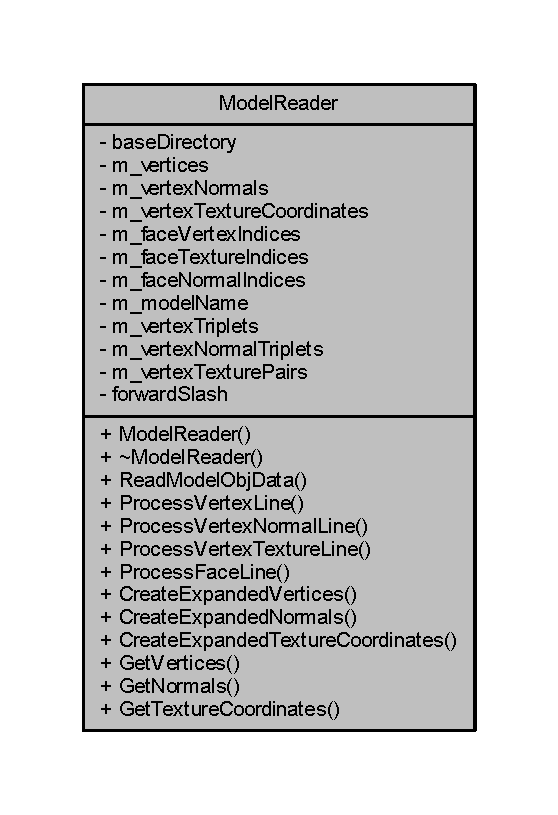
\includegraphics[width=268pt]{class_model_reader__coll__graph}
\end{center}
\end{figure}
\subsection*{Public Member Functions}
\begin{DoxyCompactItemize}
\item 
\hyperlink{class_model_reader_a9bcdfff98ff58c99dd089e4255a1e6a4}{Model\+Reader} (std\+::string s\+File\+Name)
\item 
\hyperlink{class_model_reader_a0ca7f69aa1af0ab52c43d83e8c0537de}{$\sim$\+Model\+Reader} ()
\item 
void \hyperlink{class_model_reader_a18575bb00920a495f718bdaea32d88d1}{Read\+Model\+Obj\+Data} (std\+::string s\+File\+Name)
\item 
void \hyperlink{class_model_reader_ab35aabd01b36f0f73849aa5d37269134}{Process\+Vertex\+Line} (std\+::istringstream \&iss)
\item 
void \hyperlink{class_model_reader_a4b70b7ce8745610b9c86cd30323827cf}{Process\+Vertex\+Normal\+Line} (std\+::istringstream \&iss)
\item 
void \hyperlink{class_model_reader_a937ab0dbfc1a7e45c200e8a0b520d677}{Process\+Vertex\+Texture\+Line} (std\+::istringstream \&iss)
\item 
void \hyperlink{class_model_reader_a4c89991dbe92b0adf34268e31ea249b4}{Process\+Face\+Line} (std\+::istringstream \&iss)
\item 
void \hyperlink{class_model_reader_ad488c2815537bdf59e67b5ea221c47f6}{Create\+Expanded\+Vertices} ()
\item 
void \hyperlink{class_model_reader_ada5347a6bc15931c74de786a6ccf51cc}{Create\+Expanded\+Normals} ()
\item 
void \hyperlink{class_model_reader_a08bf36b69771fea54a64c125af0dbf2f}{Create\+Expanded\+Texture\+Coordinates} ()
\item 
std\+::vector$<$ float $>$ \& \hyperlink{class_model_reader_acc0661952677fedcd92ac4d39eadc281}{Get\+Vertices} ()
\item 
std\+::vector$<$ float $>$ \& \hyperlink{class_model_reader_af72dcd34b82460711d6d1d56405ef532}{Get\+Normals} ()
\item 
std\+::vector$<$ float $>$ \& \hyperlink{class_model_reader_a041db1896d8ce51f653ba1590847de17}{Get\+Texture\+Coordinates} ()
\end{DoxyCompactItemize}
\subsection*{Private Attributes}
\begin{DoxyCompactItemize}
\item 
std\+::string \hyperlink{class_model_reader_a93d23aa8d615c4c59dd45112e09273fc}{base\+Directory}
\item 
std\+::vector$<$ float $>$ \hyperlink{class_model_reader_a31bedc9d7bcfcb8385dab2538a9fe901}{m\+\_\+vertices}
\item 
std\+::vector$<$ float $>$ \hyperlink{class_model_reader_adaf9095e7b9d76761142e1addcb7b203}{m\+\_\+vertex\+Normals}
\item 
std\+::vector$<$ float $>$ \hyperlink{class_model_reader_a650f9b20143951a5baa47d35b6b069ce}{m\+\_\+vertex\+Texture\+Coordinates}
\item 
std\+::vector$<$ unsigned int $>$ \hyperlink{class_model_reader_a9c06d6c9bbadaebcb4c9e252c1ee91f9}{m\+\_\+face\+Vertex\+Indices}
\item 
std\+::vector$<$ unsigned int $>$ \hyperlink{class_model_reader_ae39f1d039babc141dd5762cce97849e7}{m\+\_\+face\+Texture\+Indices}
\item 
std\+::vector$<$ unsigned int $>$ \hyperlink{class_model_reader_a8063140b52f022f32ff26e5ef504f1e4}{m\+\_\+face\+Normal\+Indices}
\item 
std\+::string \hyperlink{class_model_reader_a5adca8aa3aeda91670b3d5d080165b2f}{m\+\_\+model\+Name}
\item 
std\+::vector$<$ float $>$ \hyperlink{class_model_reader_a383b63a003d95c976c2abdf6acd96f90}{m\+\_\+vertex\+Triplets}
\item 
std\+::vector$<$ float $>$ \hyperlink{class_model_reader_ac53d337835121e29acf367aee4e4d407}{m\+\_\+vertex\+Normal\+Triplets}
\item 
std\+::vector$<$ float $>$ \hyperlink{class_model_reader_a1645f9266005e6ba037ff18fd95a14e2}{m\+\_\+vertex\+Texture\+Pairs}
\end{DoxyCompactItemize}
\subsection*{Static Private Attributes}
\begin{DoxyCompactItemize}
\item 
static const int \hyperlink{class_model_reader_a869fdfcdef0938fd7c06a0c35ee53488}{forward\+Slash} = 0x2F
\end{DoxyCompactItemize}


\subsection{Detailed Description}
This class is used to read models. 

\subsection{Constructor \& Destructor Documentation}
\index{Model\+Reader@{Model\+Reader}!Model\+Reader@{Model\+Reader}}
\index{Model\+Reader@{Model\+Reader}!Model\+Reader@{Model\+Reader}}
\subsubsection[{\texorpdfstring{Model\+Reader(std\+::string s\+File\+Name)}{ModelReader(std::string sFileName)}}]{\setlength{\rightskip}{0pt plus 5cm}Model\+Reader\+::\+Model\+Reader (
\begin{DoxyParamCaption}
\item[{std\+::string}]{s\+File\+Name}
\end{DoxyParamCaption}
)}\hypertarget{class_model_reader_a9bcdfff98ff58c99dd089e4255a1e6a4}{}\label{class_model_reader_a9bcdfff98ff58c99dd089e4255a1e6a4}

\begin{DoxyParams}{Parameters}
{\em s\+File\+Name} & = Name of a file. \\
\hline
\end{DoxyParams}
\index{Model\+Reader@{Model\+Reader}!````~Model\+Reader@{$\sim$\+Model\+Reader}}
\index{````~Model\+Reader@{$\sim$\+Model\+Reader}!Model\+Reader@{Model\+Reader}}
\subsubsection[{\texorpdfstring{$\sim$\+Model\+Reader()}{~ModelReader()}}]{\setlength{\rightskip}{0pt plus 5cm}Model\+Reader\+::$\sim$\+Model\+Reader (
\begin{DoxyParamCaption}
{}
\end{DoxyParamCaption}
)\hspace{0.3cm}{\ttfamily [inline]}}\hypertarget{class_model_reader_a0ca7f69aa1af0ab52c43d83e8c0537de}{}\label{class_model_reader_a0ca7f69aa1af0ab52c43d83e8c0537de}
Desctructor. 

Here is the call graph for this function\+:\nopagebreak
\begin{figure}[H]
\begin{center}
\leavevmode
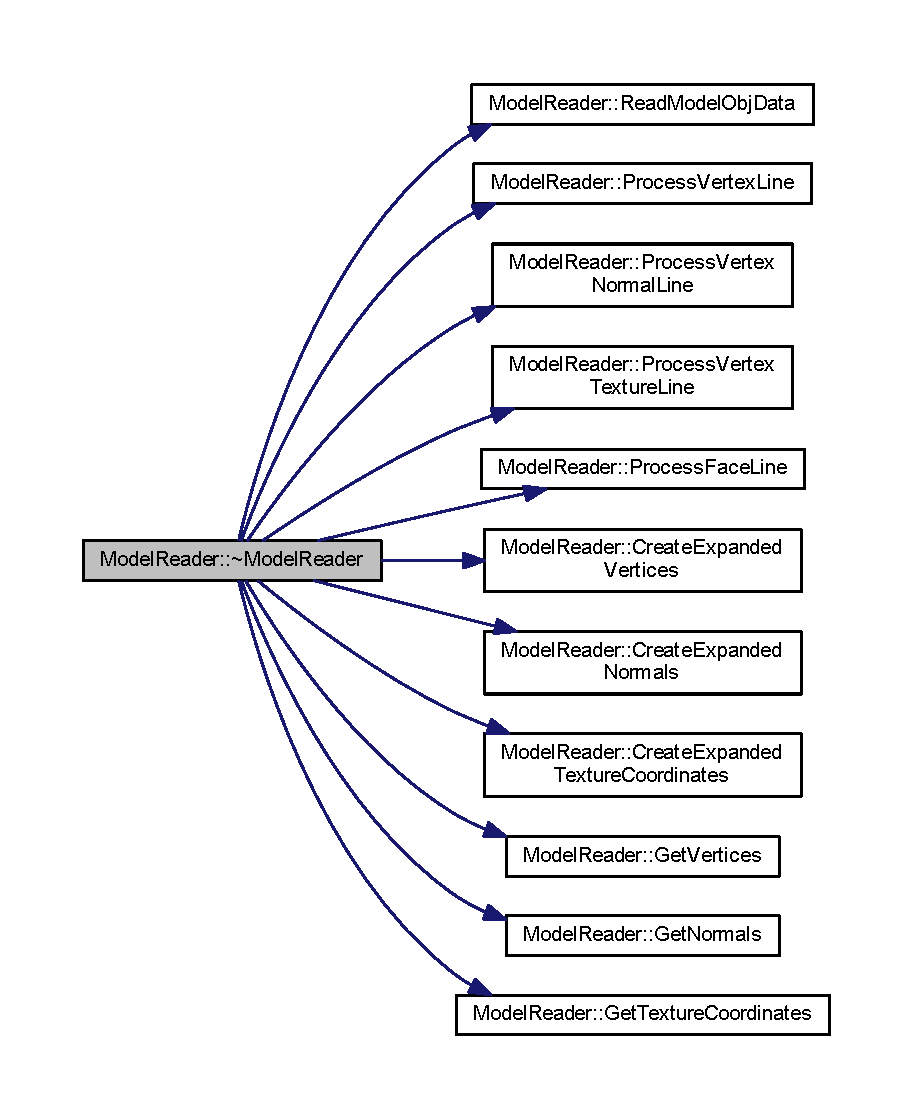
\includegraphics[width=350pt]{class_model_reader_a0ca7f69aa1af0ab52c43d83e8c0537de_cgraph}
\end{center}
\end{figure}




\subsection{Member Function Documentation}
\index{Model\+Reader@{Model\+Reader}!Create\+Expanded\+Normals@{Create\+Expanded\+Normals}}
\index{Create\+Expanded\+Normals@{Create\+Expanded\+Normals}!Model\+Reader@{Model\+Reader}}
\subsubsection[{\texorpdfstring{Create\+Expanded\+Normals()}{CreateExpandedNormals()}}]{\setlength{\rightskip}{0pt plus 5cm}void Model\+Reader\+::\+Create\+Expanded\+Normals (
\begin{DoxyParamCaption}
{}
\end{DoxyParamCaption}
)}\hypertarget{class_model_reader_ada5347a6bc15931c74de786a6ccf51cc}{}\label{class_model_reader_ada5347a6bc15931c74de786a6ccf51cc}
Creates expanded normals for Open\+Gl to read. \index{Model\+Reader@{Model\+Reader}!Create\+Expanded\+Texture\+Coordinates@{Create\+Expanded\+Texture\+Coordinates}}
\index{Create\+Expanded\+Texture\+Coordinates@{Create\+Expanded\+Texture\+Coordinates}!Model\+Reader@{Model\+Reader}}
\subsubsection[{\texorpdfstring{Create\+Expanded\+Texture\+Coordinates()}{CreateExpandedTextureCoordinates()}}]{\setlength{\rightskip}{0pt plus 5cm}void Model\+Reader\+::\+Create\+Expanded\+Texture\+Coordinates (
\begin{DoxyParamCaption}
{}
\end{DoxyParamCaption}
)}\hypertarget{class_model_reader_a08bf36b69771fea54a64c125af0dbf2f}{}\label{class_model_reader_a08bf36b69771fea54a64c125af0dbf2f}
Creates expanded texture coordinates for Open\+Gl to read. \index{Model\+Reader@{Model\+Reader}!Create\+Expanded\+Vertices@{Create\+Expanded\+Vertices}}
\index{Create\+Expanded\+Vertices@{Create\+Expanded\+Vertices}!Model\+Reader@{Model\+Reader}}
\subsubsection[{\texorpdfstring{Create\+Expanded\+Vertices()}{CreateExpandedVertices()}}]{\setlength{\rightskip}{0pt plus 5cm}void Model\+Reader\+::\+Create\+Expanded\+Vertices (
\begin{DoxyParamCaption}
{}
\end{DoxyParamCaption}
)}\hypertarget{class_model_reader_ad488c2815537bdf59e67b5ea221c47f6}{}\label{class_model_reader_ad488c2815537bdf59e67b5ea221c47f6}
Creates expanded vertices for Open\+Gl to read. \index{Model\+Reader@{Model\+Reader}!Get\+Normals@{Get\+Normals}}
\index{Get\+Normals@{Get\+Normals}!Model\+Reader@{Model\+Reader}}
\subsubsection[{\texorpdfstring{Get\+Normals()}{GetNormals()}}]{\setlength{\rightskip}{0pt plus 5cm}std\+::vector$<$float$>$\& Model\+Reader\+::\+Get\+Normals (
\begin{DoxyParamCaption}
{}
\end{DoxyParamCaption}
)}\hypertarget{class_model_reader_af72dcd34b82460711d6d1d56405ef532}{}\label{class_model_reader_af72dcd34b82460711d6d1d56405ef532}
Read normals. \begin{DoxyReturn}{Returns}
m\+\_\+vertex\+Triplets = Returns vector of normals. 
\end{DoxyReturn}
\index{Model\+Reader@{Model\+Reader}!Get\+Texture\+Coordinates@{Get\+Texture\+Coordinates}}
\index{Get\+Texture\+Coordinates@{Get\+Texture\+Coordinates}!Model\+Reader@{Model\+Reader}}
\subsubsection[{\texorpdfstring{Get\+Texture\+Coordinates()}{GetTextureCoordinates()}}]{\setlength{\rightskip}{0pt plus 5cm}std\+::vector$<$float$>$\& Model\+Reader\+::\+Get\+Texture\+Coordinates (
\begin{DoxyParamCaption}
{}
\end{DoxyParamCaption}
)}\hypertarget{class_model_reader_a041db1896d8ce51f653ba1590847de17}{}\label{class_model_reader_a041db1896d8ce51f653ba1590847de17}
Read texture coordinates. \begin{DoxyReturn}{Returns}
m\+\_\+vertex\+Triplets = Returnes vector of texture coordinates. 
\end{DoxyReturn}
\index{Model\+Reader@{Model\+Reader}!Get\+Vertices@{Get\+Vertices}}
\index{Get\+Vertices@{Get\+Vertices}!Model\+Reader@{Model\+Reader}}
\subsubsection[{\texorpdfstring{Get\+Vertices()}{GetVertices()}}]{\setlength{\rightskip}{0pt plus 5cm}std\+::vector$<$float$>$\& Model\+Reader\+::\+Get\+Vertices (
\begin{DoxyParamCaption}
{}
\end{DoxyParamCaption}
)}\hypertarget{class_model_reader_acc0661952677fedcd92ac4d39eadc281}{}\label{class_model_reader_acc0661952677fedcd92ac4d39eadc281}
Read vertices. \begin{DoxyReturn}{Returns}
m\+\_\+vertex\+Triplets = Returns vector of vertices. 
\end{DoxyReturn}
\index{Model\+Reader@{Model\+Reader}!Process\+Face\+Line@{Process\+Face\+Line}}
\index{Process\+Face\+Line@{Process\+Face\+Line}!Model\+Reader@{Model\+Reader}}
\subsubsection[{\texorpdfstring{Process\+Face\+Line(std\+::istringstream \&iss)}{ProcessFaceLine(std::istringstream &iss)}}]{\setlength{\rightskip}{0pt plus 5cm}void Model\+Reader\+::\+Process\+Face\+Line (
\begin{DoxyParamCaption}
\item[{std\+::istringstream \&}]{iss}
\end{DoxyParamCaption}
)}\hypertarget{class_model_reader_a4c89991dbe92b0adf34268e31ea249b4}{}\label{class_model_reader_a4c89991dbe92b0adf34268e31ea249b4}
Processes face when encounters F. 
\begin{DoxyParams}{Parameters}
{\em iss} & = Line input with a face. \\
\hline
\end{DoxyParams}
\index{Model\+Reader@{Model\+Reader}!Process\+Vertex\+Line@{Process\+Vertex\+Line}}
\index{Process\+Vertex\+Line@{Process\+Vertex\+Line}!Model\+Reader@{Model\+Reader}}
\subsubsection[{\texorpdfstring{Process\+Vertex\+Line(std\+::istringstream \&iss)}{ProcessVertexLine(std::istringstream &iss)}}]{\setlength{\rightskip}{0pt plus 5cm}void Model\+Reader\+::\+Process\+Vertex\+Line (
\begin{DoxyParamCaption}
\item[{std\+::istringstream \&}]{iss}
\end{DoxyParamCaption}
)}\hypertarget{class_model_reader_ab35aabd01b36f0f73849aa5d37269134}{}\label{class_model_reader_ab35aabd01b36f0f73849aa5d37269134}
Processes vertex when encounters V. 
\begin{DoxyParams}{Parameters}
{\em iss} & = Line input with vertex. \\
\hline
\end{DoxyParams}
\index{Model\+Reader@{Model\+Reader}!Process\+Vertex\+Normal\+Line@{Process\+Vertex\+Normal\+Line}}
\index{Process\+Vertex\+Normal\+Line@{Process\+Vertex\+Normal\+Line}!Model\+Reader@{Model\+Reader}}
\subsubsection[{\texorpdfstring{Process\+Vertex\+Normal\+Line(std\+::istringstream \&iss)}{ProcessVertexNormalLine(std::istringstream &iss)}}]{\setlength{\rightskip}{0pt plus 5cm}void Model\+Reader\+::\+Process\+Vertex\+Normal\+Line (
\begin{DoxyParamCaption}
\item[{std\+::istringstream \&}]{iss}
\end{DoxyParamCaption}
)}\hypertarget{class_model_reader_a4b70b7ce8745610b9c86cd30323827cf}{}\label{class_model_reader_a4b70b7ce8745610b9c86cd30323827cf}
Processes vertex when encounters VN. 
\begin{DoxyParams}{Parameters}
{\em iss} & = Line input with normal. \\
\hline
\end{DoxyParams}
\index{Model\+Reader@{Model\+Reader}!Process\+Vertex\+Texture\+Line@{Process\+Vertex\+Texture\+Line}}
\index{Process\+Vertex\+Texture\+Line@{Process\+Vertex\+Texture\+Line}!Model\+Reader@{Model\+Reader}}
\subsubsection[{\texorpdfstring{Process\+Vertex\+Texture\+Line(std\+::istringstream \&iss)}{ProcessVertexTextureLine(std::istringstream &iss)}}]{\setlength{\rightskip}{0pt plus 5cm}void Model\+Reader\+::\+Process\+Vertex\+Texture\+Line (
\begin{DoxyParamCaption}
\item[{std\+::istringstream \&}]{iss}
\end{DoxyParamCaption}
)}\hypertarget{class_model_reader_a937ab0dbfc1a7e45c200e8a0b520d677}{}\label{class_model_reader_a937ab0dbfc1a7e45c200e8a0b520d677}
Processes vertex when encounters VT. 
\begin{DoxyParams}{Parameters}
{\em iss} & = Line input with texture coordinates. \\
\hline
\end{DoxyParams}
\index{Model\+Reader@{Model\+Reader}!Read\+Model\+Obj\+Data@{Read\+Model\+Obj\+Data}}
\index{Read\+Model\+Obj\+Data@{Read\+Model\+Obj\+Data}!Model\+Reader@{Model\+Reader}}
\subsubsection[{\texorpdfstring{Read\+Model\+Obj\+Data(std\+::string s\+File\+Name)}{ReadModelObjData(std::string sFileName)}}]{\setlength{\rightskip}{0pt plus 5cm}void Model\+Reader\+::\+Read\+Model\+Obj\+Data (
\begin{DoxyParamCaption}
\item[{std\+::string}]{s\+File\+Name}
\end{DoxyParamCaption}
)}\hypertarget{class_model_reader_a18575bb00920a495f718bdaea32d88d1}{}\label{class_model_reader_a18575bb00920a495f718bdaea32d88d1}
Read the model. 
\begin{DoxyParams}{Parameters}
{\em s\+File\+Name} & = Name of a file. \\
\hline
\end{DoxyParams}


\subsection{Member Data Documentation}
\index{Model\+Reader@{Model\+Reader}!base\+Directory@{base\+Directory}}
\index{base\+Directory@{base\+Directory}!Model\+Reader@{Model\+Reader}}
\subsubsection[{\texorpdfstring{base\+Directory}{baseDirectory}}]{\setlength{\rightskip}{0pt plus 5cm}std\+::string Model\+Reader\+::base\+Directory\hspace{0.3cm}{\ttfamily [private]}}\hypertarget{class_model_reader_a93d23aa8d615c4c59dd45112e09273fc}{}\label{class_model_reader_a93d23aa8d615c4c59dd45112e09273fc}
Our base directory with models. \index{Model\+Reader@{Model\+Reader}!forward\+Slash@{forward\+Slash}}
\index{forward\+Slash@{forward\+Slash}!Model\+Reader@{Model\+Reader}}
\subsubsection[{\texorpdfstring{forward\+Slash}{forwardSlash}}]{\setlength{\rightskip}{0pt plus 5cm}const int Model\+Reader\+::forward\+Slash = 0x2F\hspace{0.3cm}{\ttfamily [static]}, {\ttfamily [private]}}\hypertarget{class_model_reader_a869fdfcdef0938fd7c06a0c35ee53488}{}\label{class_model_reader_a869fdfcdef0938fd7c06a0c35ee53488}
A\+S\+C\+II code for forward slash. \index{Model\+Reader@{Model\+Reader}!m\+\_\+face\+Normal\+Indices@{m\+\_\+face\+Normal\+Indices}}
\index{m\+\_\+face\+Normal\+Indices@{m\+\_\+face\+Normal\+Indices}!Model\+Reader@{Model\+Reader}}
\subsubsection[{\texorpdfstring{m\+\_\+face\+Normal\+Indices}{m_faceNormalIndices}}]{\setlength{\rightskip}{0pt plus 5cm}std\+::vector$<$unsigned int$>$ Model\+Reader\+::m\+\_\+face\+Normal\+Indices\hspace{0.3cm}{\ttfamily [private]}}\hypertarget{class_model_reader_a8063140b52f022f32ff26e5ef504f1e4}{}\label{class_model_reader_a8063140b52f022f32ff26e5ef504f1e4}
Face noraml indices = F // // X . \index{Model\+Reader@{Model\+Reader}!m\+\_\+face\+Texture\+Indices@{m\+\_\+face\+Texture\+Indices}}
\index{m\+\_\+face\+Texture\+Indices@{m\+\_\+face\+Texture\+Indices}!Model\+Reader@{Model\+Reader}}
\subsubsection[{\texorpdfstring{m\+\_\+face\+Texture\+Indices}{m_faceTextureIndices}}]{\setlength{\rightskip}{0pt plus 5cm}std\+::vector$<$unsigned int$>$ Model\+Reader\+::m\+\_\+face\+Texture\+Indices\hspace{0.3cm}{\ttfamily [private]}}\hypertarget{class_model_reader_ae39f1d039babc141dd5762cce97849e7}{}\label{class_model_reader_ae39f1d039babc141dd5762cce97849e7}
Face texture indices = F // X // . \index{Model\+Reader@{Model\+Reader}!m\+\_\+face\+Vertex\+Indices@{m\+\_\+face\+Vertex\+Indices}}
\index{m\+\_\+face\+Vertex\+Indices@{m\+\_\+face\+Vertex\+Indices}!Model\+Reader@{Model\+Reader}}
\subsubsection[{\texorpdfstring{m\+\_\+face\+Vertex\+Indices}{m_faceVertexIndices}}]{\setlength{\rightskip}{0pt plus 5cm}std\+::vector$<$unsigned int$>$ Model\+Reader\+::m\+\_\+face\+Vertex\+Indices\hspace{0.3cm}{\ttfamily [private]}}\hypertarget{class_model_reader_a9c06d6c9bbadaebcb4c9e252c1ee91f9}{}\label{class_model_reader_a9c06d6c9bbadaebcb4c9e252c1ee91f9}
Face vertex indices = F X // // . \index{Model\+Reader@{Model\+Reader}!m\+\_\+model\+Name@{m\+\_\+model\+Name}}
\index{m\+\_\+model\+Name@{m\+\_\+model\+Name}!Model\+Reader@{Model\+Reader}}
\subsubsection[{\texorpdfstring{m\+\_\+model\+Name}{m_modelName}}]{\setlength{\rightskip}{0pt plus 5cm}std\+::string Model\+Reader\+::m\+\_\+model\+Name\hspace{0.3cm}{\ttfamily [private]}}\hypertarget{class_model_reader_a5adca8aa3aeda91670b3d5d080165b2f}{}\label{class_model_reader_a5adca8aa3aeda91670b3d5d080165b2f}
Name of a model. \index{Model\+Reader@{Model\+Reader}!m\+\_\+vertex\+Normals@{m\+\_\+vertex\+Normals}}
\index{m\+\_\+vertex\+Normals@{m\+\_\+vertex\+Normals}!Model\+Reader@{Model\+Reader}}
\subsubsection[{\texorpdfstring{m\+\_\+vertex\+Normals}{m_vertexNormals}}]{\setlength{\rightskip}{0pt plus 5cm}std\+::vector$<$float$>$ Model\+Reader\+::m\+\_\+vertex\+Normals\hspace{0.3cm}{\ttfamily [private]}}\hypertarget{class_model_reader_adaf9095e7b9d76761142e1addcb7b203}{}\label{class_model_reader_adaf9095e7b9d76761142e1addcb7b203}
Vertex normals = VN. \index{Model\+Reader@{Model\+Reader}!m\+\_\+vertex\+Normal\+Triplets@{m\+\_\+vertex\+Normal\+Triplets}}
\index{m\+\_\+vertex\+Normal\+Triplets@{m\+\_\+vertex\+Normal\+Triplets}!Model\+Reader@{Model\+Reader}}
\subsubsection[{\texorpdfstring{m\+\_\+vertex\+Normal\+Triplets}{m_vertexNormalTriplets}}]{\setlength{\rightskip}{0pt plus 5cm}std\+::vector$<$float$>$ Model\+Reader\+::m\+\_\+vertex\+Normal\+Triplets\hspace{0.3cm}{\ttfamily [private]}}\hypertarget{class_model_reader_ac53d337835121e29acf367aee4e4d407}{}\label{class_model_reader_ac53d337835121e29acf367aee4e4d407}
Necessary data of normals for O\+P\+E\+N\+GL in readable format. \index{Model\+Reader@{Model\+Reader}!m\+\_\+vertex\+Texture\+Coordinates@{m\+\_\+vertex\+Texture\+Coordinates}}
\index{m\+\_\+vertex\+Texture\+Coordinates@{m\+\_\+vertex\+Texture\+Coordinates}!Model\+Reader@{Model\+Reader}}
\subsubsection[{\texorpdfstring{m\+\_\+vertex\+Texture\+Coordinates}{m_vertexTextureCoordinates}}]{\setlength{\rightskip}{0pt plus 5cm}std\+::vector$<$float$>$ Model\+Reader\+::m\+\_\+vertex\+Texture\+Coordinates\hspace{0.3cm}{\ttfamily [private]}}\hypertarget{class_model_reader_a650f9b20143951a5baa47d35b6b069ce}{}\label{class_model_reader_a650f9b20143951a5baa47d35b6b069ce}
Texture Coordinates = VT resctricted to UV. \index{Model\+Reader@{Model\+Reader}!m\+\_\+vertex\+Texture\+Pairs@{m\+\_\+vertex\+Texture\+Pairs}}
\index{m\+\_\+vertex\+Texture\+Pairs@{m\+\_\+vertex\+Texture\+Pairs}!Model\+Reader@{Model\+Reader}}
\subsubsection[{\texorpdfstring{m\+\_\+vertex\+Texture\+Pairs}{m_vertexTexturePairs}}]{\setlength{\rightskip}{0pt plus 5cm}std\+::vector$<$float$>$ Model\+Reader\+::m\+\_\+vertex\+Texture\+Pairs\hspace{0.3cm}{\ttfamily [private]}}\hypertarget{class_model_reader_a1645f9266005e6ba037ff18fd95a14e2}{}\label{class_model_reader_a1645f9266005e6ba037ff18fd95a14e2}
Necessary data of texture coordinates for O\+P\+E\+N\+GL in readable format. \index{Model\+Reader@{Model\+Reader}!m\+\_\+vertex\+Triplets@{m\+\_\+vertex\+Triplets}}
\index{m\+\_\+vertex\+Triplets@{m\+\_\+vertex\+Triplets}!Model\+Reader@{Model\+Reader}}
\subsubsection[{\texorpdfstring{m\+\_\+vertex\+Triplets}{m_vertexTriplets}}]{\setlength{\rightskip}{0pt plus 5cm}std\+::vector$<$float$>$ Model\+Reader\+::m\+\_\+vertex\+Triplets\hspace{0.3cm}{\ttfamily [private]}}\hypertarget{class_model_reader_a383b63a003d95c976c2abdf6acd96f90}{}\label{class_model_reader_a383b63a003d95c976c2abdf6acd96f90}
Necessary data of vertices for O\+P\+E\+N\+GL in readable format. \index{Model\+Reader@{Model\+Reader}!m\+\_\+vertices@{m\+\_\+vertices}}
\index{m\+\_\+vertices@{m\+\_\+vertices}!Model\+Reader@{Model\+Reader}}
\subsubsection[{\texorpdfstring{m\+\_\+vertices}{m_vertices}}]{\setlength{\rightskip}{0pt plus 5cm}std\+::vector$<$float$>$ Model\+Reader\+::m\+\_\+vertices\hspace{0.3cm}{\ttfamily [private]}}\hypertarget{class_model_reader_a31bedc9d7bcfcb8385dab2538a9fe901}{}\label{class_model_reader_a31bedc9d7bcfcb8385dab2538a9fe901}
Vertices = V. 

The documentation for this class was generated from the following file\+:\begin{DoxyCompactItemize}
\item 
C\+:/\+Airport/include/\hyperlink{model_reader_8h}{model\+Reader.\+h}\end{DoxyCompactItemize}

\hypertarget{class_scene}{}\section{Scene Class Reference}
\label{class_scene}\index{Scene@{Scene}}


This class is used to render a scene.  




{\ttfamily \#include $<$scene.\+h$>$}



Collaboration diagram for Scene\+:
\nopagebreak
\begin{figure}[H]
\begin{center}
\leavevmode
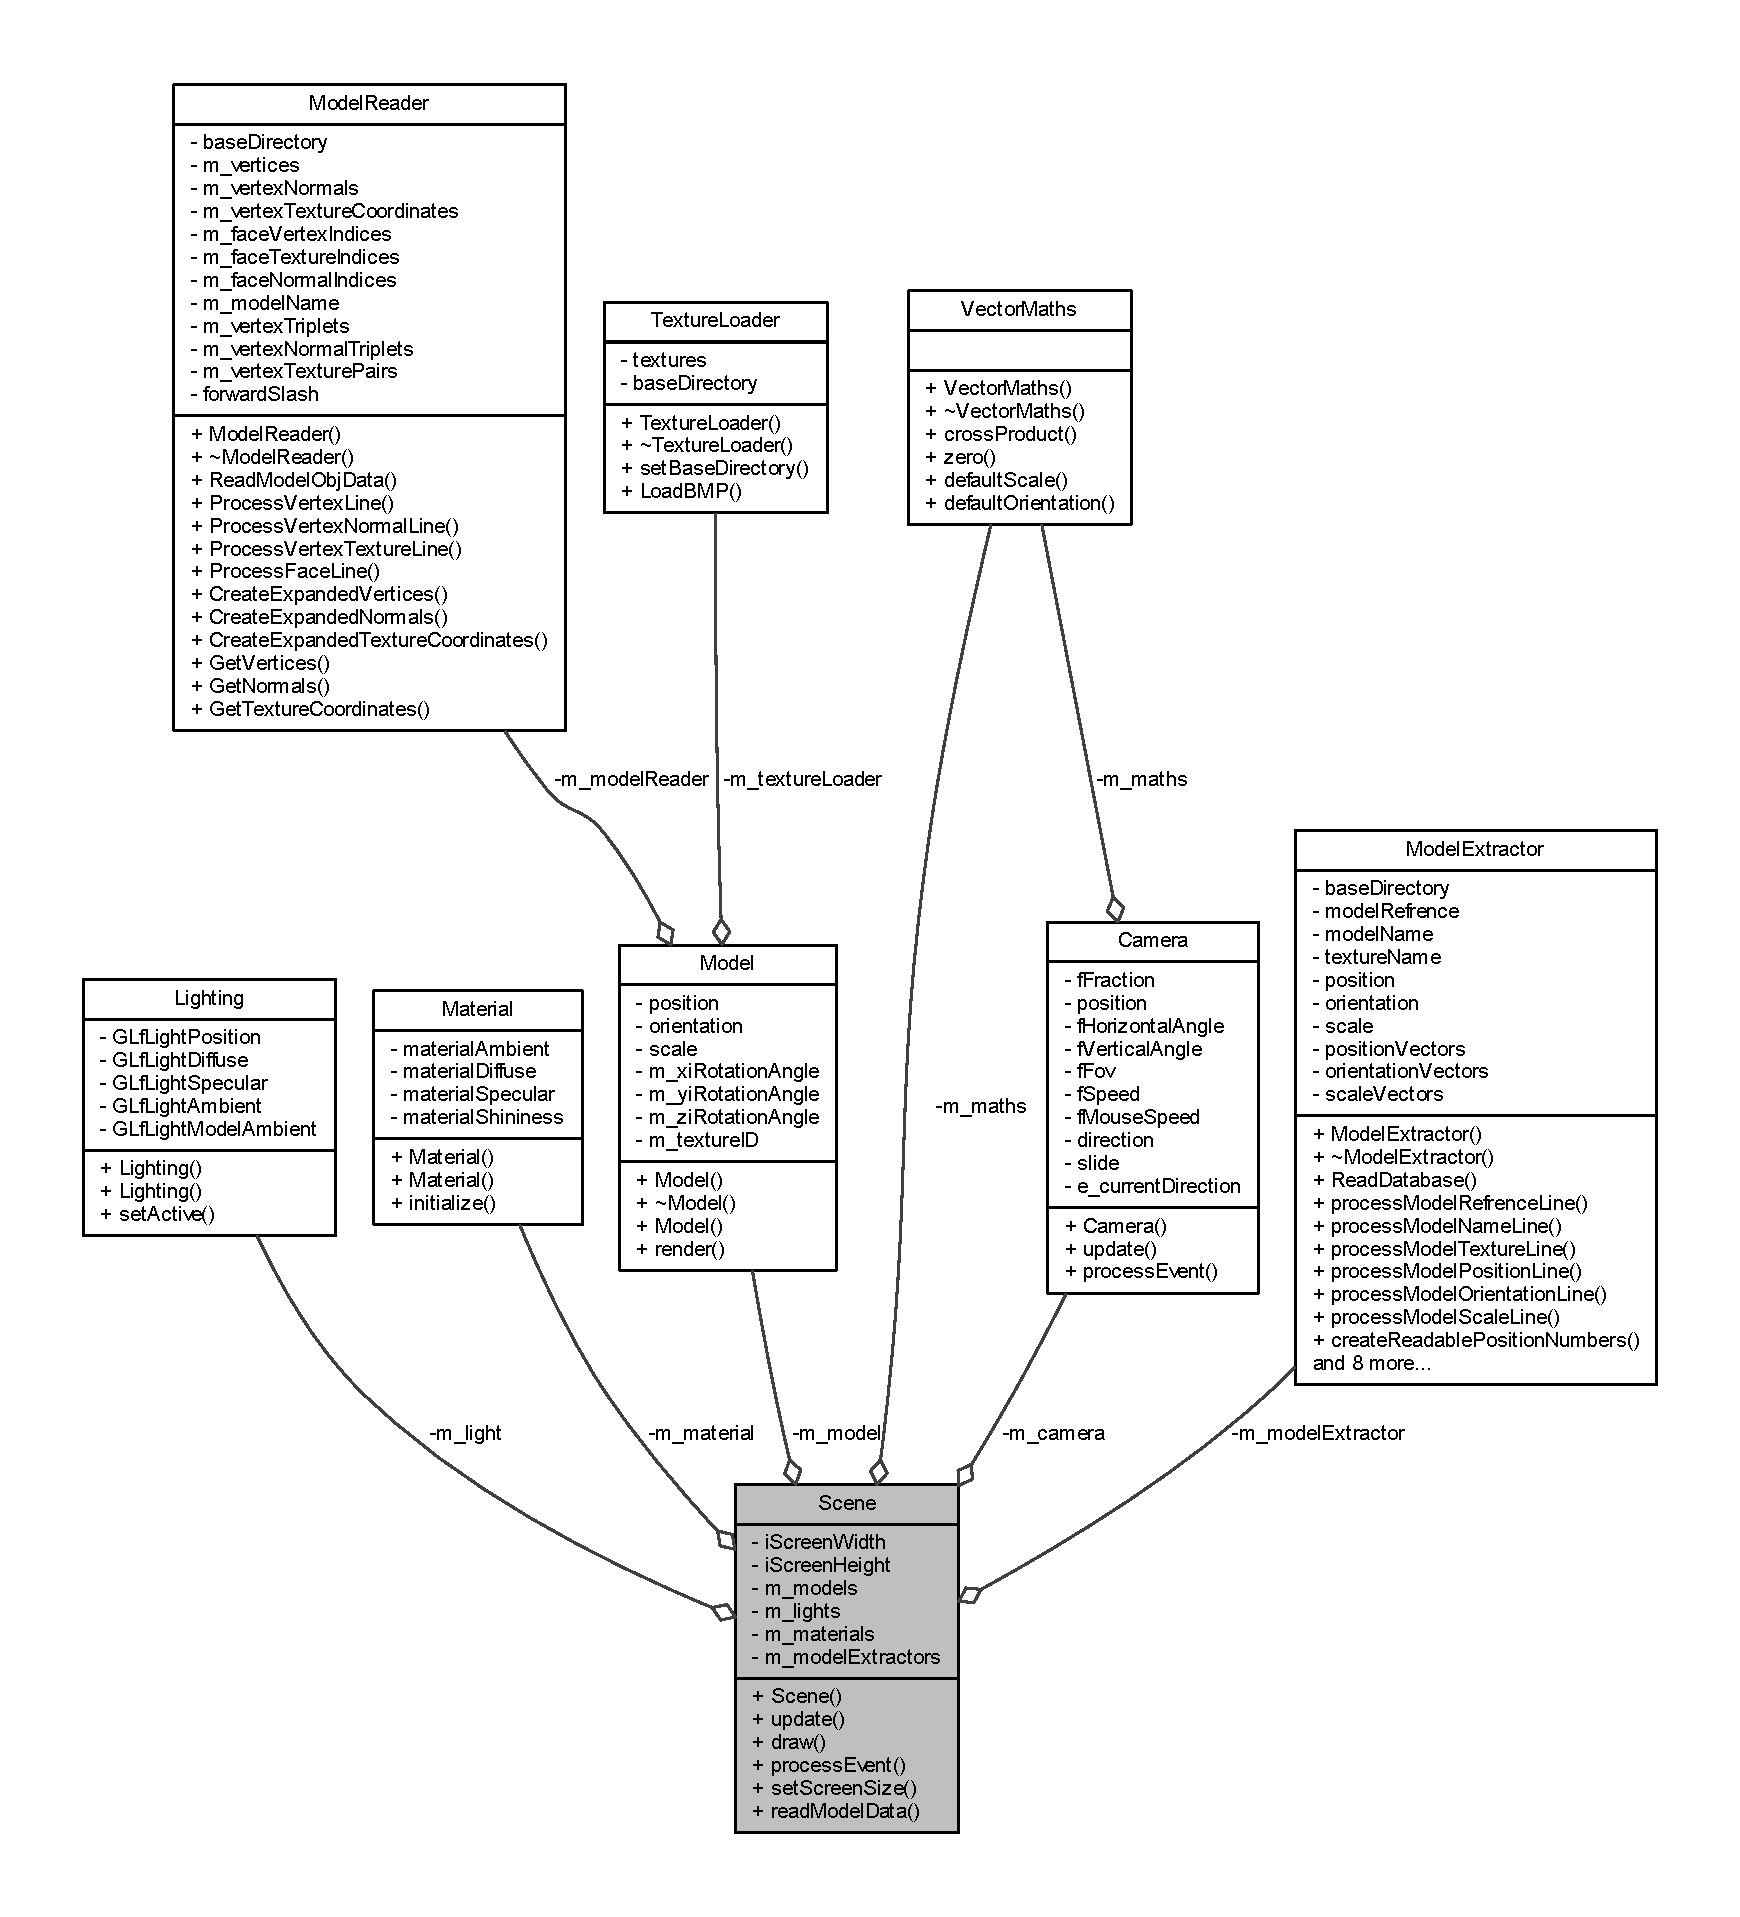
\includegraphics[width=350pt]{class_scene__coll__graph}
\end{center}
\end{figure}
\subsection*{Public Member Functions}
\begin{DoxyCompactItemize}
\item 
\hyperlink{class_scene_ad10176d75a9cc0da56626f682d083507}{Scene} ()
\item 
void \hyperlink{class_scene_a2984c9b32deff64e52a5c49744d90721}{update} (float f\+Elapsed\+Time, sf\+::\+Vector2i i\+Mouse\+Position)
\item 
void \hyperlink{class_scene_ac0e3d2c98ba6063a086467fb2c19142f}{draw} ()
\item 
void \hyperlink{class_scene_ab489a784acb0f14e1649f3970ea49195}{process\+Event} (sf\+::\+Event \&e, sf\+::\+Window \&window)
\item 
void \hyperlink{class_scene_aaffb708da35121468f9a66c626881052}{set\+Screen\+Size} (int \hyperlink{class_scene_a778137dcab836e6be4217615873db576}{i\+Screen\+Width}, int \hyperlink{class_scene_aac44019cbb3024de33132b0f278708f9}{i\+Screen\+Height})
\item 
void \hyperlink{class_scene_ac6c60d8e20f167e468e4bf5dc17ca68e}{read\+Model\+Data} (\hyperlink{class_model_extractor}{Model\+Extractor} $\ast$reader, std\+::vector$<$ \hyperlink{class_model}{Model} $>$ \&models)
\end{DoxyCompactItemize}
\subsection*{Private Attributes}
\begin{DoxyCompactItemize}
\item 
int \hyperlink{class_scene_a778137dcab836e6be4217615873db576}{i\+Screen\+Width}
\item 
int \hyperlink{class_scene_aac44019cbb3024de33132b0f278708f9}{i\+Screen\+Height}
\item 
\hyperlink{class_camera}{Camera} \hyperlink{class_scene_a1b706ed302145fe191131cefe8873fec}{m\+\_\+camera}
\item 
\hyperlink{class_model}{Model} \hyperlink{class_scene_a8398e5ee10d0a39903a26d665f3f3a9f}{m\+\_\+model}
\item 
\hyperlink{class_lighting}{Lighting} \hyperlink{class_scene_af2eaac7f7e7997e0b2a47373f55cb2e1}{m\+\_\+light}
\item 
\hyperlink{class_material}{Material} \hyperlink{class_scene_a80eed5a8d1800f3b426bca2eda26d4b6}{m\+\_\+material}
\item 
\hyperlink{class_model_extractor}{Model\+Extractor} \hyperlink{class_scene_aadd2050cd69c19889b146c6334feb8dd}{m\+\_\+model\+Extractor}
\item 
std\+::array$<$ std\+::vector$<$ \hyperlink{class_model}{Model} $>$, 2 $>$ \hyperlink{class_scene_a10335e874947752239a933d35d926c3b}{m\+\_\+models}
\item 
std\+::array$<$ \hyperlink{class_lighting}{Lighting}, 1 $>$ \hyperlink{class_scene_adb68e0b4186fa78d472880f259e49671}{m\+\_\+lights}
\item 
std\+::array$<$ \hyperlink{class_material}{Material}, 2 $>$ \hyperlink{class_scene_af5fcdd7b94d1669008bd13d7ecde01c1}{m\+\_\+materials}
\item 
std\+::array$<$ \hyperlink{class_model_extractor}{Model\+Extractor} $\ast$, 2 $>$ \hyperlink{class_scene_a023c55afb84b247b9c51f6d33131102c}{m\+\_\+model\+Extractors}
\item 
\hyperlink{class_vector_maths}{Vector\+Maths} \hyperlink{class_scene_a64101e7e0ed72202c9898a5eddf28a7d}{m\+\_\+maths}
\end{DoxyCompactItemize}


\subsection{Detailed Description}
This class is used to render a scene. 

\subsection{Constructor \& Destructor Documentation}
\index{Scene@{Scene}!Scene@{Scene}}
\index{Scene@{Scene}!Scene@{Scene}}
\subsubsection[{\texorpdfstring{Scene()}{Scene()}}]{\setlength{\rightskip}{0pt plus 5cm}Scene\+::\+Scene (
\begin{DoxyParamCaption}
{}
\end{DoxyParamCaption}
)}\hypertarget{class_scene_ad10176d75a9cc0da56626f682d083507}{}\label{class_scene_ad10176d75a9cc0da56626f682d083507}


\subsection{Member Function Documentation}
\index{Scene@{Scene}!draw@{draw}}
\index{draw@{draw}!Scene@{Scene}}
\subsubsection[{\texorpdfstring{draw()}{draw()}}]{\setlength{\rightskip}{0pt plus 5cm}void Scene\+::draw (
\begin{DoxyParamCaption}
{}
\end{DoxyParamCaption}
)}\hypertarget{class_scene_ac0e3d2c98ba6063a086467fb2c19142f}{}\label{class_scene_ac0e3d2c98ba6063a086467fb2c19142f}
\index{Scene@{Scene}!process\+Event@{process\+Event}}
\index{process\+Event@{process\+Event}!Scene@{Scene}}
\subsubsection[{\texorpdfstring{process\+Event(sf\+::\+Event \&e, sf\+::\+Window \&window)}{processEvent(sf::Event &e, sf::Window &window)}}]{\setlength{\rightskip}{0pt plus 5cm}void Scene\+::process\+Event (
\begin{DoxyParamCaption}
\item[{sf\+::\+Event \&}]{e, }
\item[{sf\+::\+Window \&}]{window}
\end{DoxyParamCaption}
)}\hypertarget{class_scene_ab489a784acb0f14e1649f3970ea49195}{}\label{class_scene_ab489a784acb0f14e1649f3970ea49195}

\begin{DoxyParams}{Parameters}
{\em e} & = event. \\
\hline
{\em window} & = Our window. \\
\hline
\end{DoxyParams}
\index{Scene@{Scene}!read\+Model\+Data@{read\+Model\+Data}}
\index{read\+Model\+Data@{read\+Model\+Data}!Scene@{Scene}}
\subsubsection[{\texorpdfstring{read\+Model\+Data(\+Model\+Extractor $\ast$reader, std\+::vector$<$ Model $>$ \&models)}{readModelData(ModelExtractor *reader, std::vector< Model > &models)}}]{\setlength{\rightskip}{0pt plus 5cm}void Scene\+::read\+Model\+Data (
\begin{DoxyParamCaption}
\item[{{\bf Model\+Extractor} $\ast$}]{reader, }
\item[{std\+::vector$<$ {\bf Model} $>$ \&}]{models}
\end{DoxyParamCaption}
)}\hypertarget{class_scene_ac6c60d8e20f167e468e4bf5dc17ca68e}{}\label{class_scene_ac6c60d8e20f167e468e4bf5dc17ca68e}

\begin{DoxyParams}{Parameters}
{\em reader} & = Read the model data. \\
\hline
{\em models} & = Vector of models. \\
\hline
\end{DoxyParams}
\index{Scene@{Scene}!set\+Screen\+Size@{set\+Screen\+Size}}
\index{set\+Screen\+Size@{set\+Screen\+Size}!Scene@{Scene}}
\subsubsection[{\texorpdfstring{set\+Screen\+Size(int i\+Screen\+Width, int i\+Screen\+Height)}{setScreenSize(int iScreenWidth, int iScreenHeight)}}]{\setlength{\rightskip}{0pt plus 5cm}void Scene\+::set\+Screen\+Size (
\begin{DoxyParamCaption}
\item[{int}]{i\+Screen\+Width, }
\item[{int}]{i\+Screen\+Height}
\end{DoxyParamCaption}
)}\hypertarget{class_scene_aaffb708da35121468f9a66c626881052}{}\label{class_scene_aaffb708da35121468f9a66c626881052}

\begin{DoxyParams}{Parameters}
{\em i\+Screen\+Width} & = Screen width. \\
\hline
{\em i\+Screen\+Height} & = Screen height. \\
\hline
\end{DoxyParams}
\index{Scene@{Scene}!update@{update}}
\index{update@{update}!Scene@{Scene}}
\subsubsection[{\texorpdfstring{update(float f\+Elapsed\+Time, sf\+::\+Vector2i i\+Mouse\+Position)}{update(float fElapsedTime, sf::Vector2i iMousePosition)}}]{\setlength{\rightskip}{0pt plus 5cm}void Scene\+::update (
\begin{DoxyParamCaption}
\item[{float}]{f\+Elapsed\+Time, }
\item[{sf\+::\+Vector2i}]{i\+Mouse\+Position}
\end{DoxyParamCaption}
)}\hypertarget{class_scene_a2984c9b32deff64e52a5c49744d90721}{}\label{class_scene_a2984c9b32deff64e52a5c49744d90721}
Update the scene. 
\begin{DoxyParams}{Parameters}
{\em f\+Elapesed\+Time} & = Refresh rate. \\
\hline
{\em i\+Mouse\+Position} & = Position of a mouse. \\
\hline
\end{DoxyParams}


\subsection{Member Data Documentation}
\index{Scene@{Scene}!i\+Screen\+Height@{i\+Screen\+Height}}
\index{i\+Screen\+Height@{i\+Screen\+Height}!Scene@{Scene}}
\subsubsection[{\texorpdfstring{i\+Screen\+Height}{iScreenHeight}}]{\setlength{\rightskip}{0pt plus 5cm}int Scene\+::i\+Screen\+Height\hspace{0.3cm}{\ttfamily [private]}}\hypertarget{class_scene_aac44019cbb3024de33132b0f278708f9}{}\label{class_scene_aac44019cbb3024de33132b0f278708f9}
Screen height. \index{Scene@{Scene}!i\+Screen\+Width@{i\+Screen\+Width}}
\index{i\+Screen\+Width@{i\+Screen\+Width}!Scene@{Scene}}
\subsubsection[{\texorpdfstring{i\+Screen\+Width}{iScreenWidth}}]{\setlength{\rightskip}{0pt plus 5cm}int Scene\+::i\+Screen\+Width\hspace{0.3cm}{\ttfamily [private]}}\hypertarget{class_scene_a778137dcab836e6be4217615873db576}{}\label{class_scene_a778137dcab836e6be4217615873db576}
Screen width. \index{Scene@{Scene}!m\+\_\+camera@{m\+\_\+camera}}
\index{m\+\_\+camera@{m\+\_\+camera}!Scene@{Scene}}
\subsubsection[{\texorpdfstring{m\+\_\+camera}{m_camera}}]{\setlength{\rightskip}{0pt plus 5cm}{\bf Camera} Scene\+::m\+\_\+camera\hspace{0.3cm}{\ttfamily [private]}}\hypertarget{class_scene_a1b706ed302145fe191131cefe8873fec}{}\label{class_scene_a1b706ed302145fe191131cefe8873fec}
Our camera. \index{Scene@{Scene}!m\+\_\+light@{m\+\_\+light}}
\index{m\+\_\+light@{m\+\_\+light}!Scene@{Scene}}
\subsubsection[{\texorpdfstring{m\+\_\+light}{m_light}}]{\setlength{\rightskip}{0pt plus 5cm}{\bf Lighting} Scene\+::m\+\_\+light\hspace{0.3cm}{\ttfamily [private]}}\hypertarget{class_scene_af2eaac7f7e7997e0b2a47373f55cb2e1}{}\label{class_scene_af2eaac7f7e7997e0b2a47373f55cb2e1}
\index{Scene@{Scene}!m\+\_\+lights@{m\+\_\+lights}}
\index{m\+\_\+lights@{m\+\_\+lights}!Scene@{Scene}}
\subsubsection[{\texorpdfstring{m\+\_\+lights}{m_lights}}]{\setlength{\rightskip}{0pt plus 5cm}std\+::array$<${\bf Lighting}, 1$>$ Scene\+::m\+\_\+lights\hspace{0.3cm}{\ttfamily [private]}}\hypertarget{class_scene_adb68e0b4186fa78d472880f259e49671}{}\label{class_scene_adb68e0b4186fa78d472880f259e49671}
\index{Scene@{Scene}!m\+\_\+material@{m\+\_\+material}}
\index{m\+\_\+material@{m\+\_\+material}!Scene@{Scene}}
\subsubsection[{\texorpdfstring{m\+\_\+material}{m_material}}]{\setlength{\rightskip}{0pt plus 5cm}{\bf Material} Scene\+::m\+\_\+material\hspace{0.3cm}{\ttfamily [private]}}\hypertarget{class_scene_a80eed5a8d1800f3b426bca2eda26d4b6}{}\label{class_scene_a80eed5a8d1800f3b426bca2eda26d4b6}
\index{Scene@{Scene}!m\+\_\+materials@{m\+\_\+materials}}
\index{m\+\_\+materials@{m\+\_\+materials}!Scene@{Scene}}
\subsubsection[{\texorpdfstring{m\+\_\+materials}{m_materials}}]{\setlength{\rightskip}{0pt plus 5cm}std\+::array$<${\bf Material}, 2$>$ Scene\+::m\+\_\+materials\hspace{0.3cm}{\ttfamily [private]}}\hypertarget{class_scene_af5fcdd7b94d1669008bd13d7ecde01c1}{}\label{class_scene_af5fcdd7b94d1669008bd13d7ecde01c1}
\index{Scene@{Scene}!m\+\_\+maths@{m\+\_\+maths}}
\index{m\+\_\+maths@{m\+\_\+maths}!Scene@{Scene}}
\subsubsection[{\texorpdfstring{m\+\_\+maths}{m_maths}}]{\setlength{\rightskip}{0pt plus 5cm}{\bf Vector\+Maths} Scene\+::m\+\_\+maths\hspace{0.3cm}{\ttfamily [private]}}\hypertarget{class_scene_a64101e7e0ed72202c9898a5eddf28a7d}{}\label{class_scene_a64101e7e0ed72202c9898a5eddf28a7d}
\index{Scene@{Scene}!m\+\_\+model@{m\+\_\+model}}
\index{m\+\_\+model@{m\+\_\+model}!Scene@{Scene}}
\subsubsection[{\texorpdfstring{m\+\_\+model}{m_model}}]{\setlength{\rightskip}{0pt plus 5cm}{\bf Model} Scene\+::m\+\_\+model\hspace{0.3cm}{\ttfamily [private]}}\hypertarget{class_scene_a8398e5ee10d0a39903a26d665f3f3a9f}{}\label{class_scene_a8398e5ee10d0a39903a26d665f3f3a9f}
\index{Scene@{Scene}!m\+\_\+model\+Extractor@{m\+\_\+model\+Extractor}}
\index{m\+\_\+model\+Extractor@{m\+\_\+model\+Extractor}!Scene@{Scene}}
\subsubsection[{\texorpdfstring{m\+\_\+model\+Extractor}{m_modelExtractor}}]{\setlength{\rightskip}{0pt plus 5cm}{\bf Model\+Extractor} Scene\+::m\+\_\+model\+Extractor\hspace{0.3cm}{\ttfamily [private]}}\hypertarget{class_scene_aadd2050cd69c19889b146c6334feb8dd}{}\label{class_scene_aadd2050cd69c19889b146c6334feb8dd}
\index{Scene@{Scene}!m\+\_\+model\+Extractors@{m\+\_\+model\+Extractors}}
\index{m\+\_\+model\+Extractors@{m\+\_\+model\+Extractors}!Scene@{Scene}}
\subsubsection[{\texorpdfstring{m\+\_\+model\+Extractors}{m_modelExtractors}}]{\setlength{\rightskip}{0pt plus 5cm}std\+::array$<${\bf Model\+Extractor}$\ast$, 2$>$ Scene\+::m\+\_\+model\+Extractors\hspace{0.3cm}{\ttfamily [private]}}\hypertarget{class_scene_a023c55afb84b247b9c51f6d33131102c}{}\label{class_scene_a023c55afb84b247b9c51f6d33131102c}
\index{Scene@{Scene}!m\+\_\+models@{m\+\_\+models}}
\index{m\+\_\+models@{m\+\_\+models}!Scene@{Scene}}
\subsubsection[{\texorpdfstring{m\+\_\+models}{m_models}}]{\setlength{\rightskip}{0pt plus 5cm}std\+::array$<$std\+::vector$<${\bf Model}$>$, 2$>$ Scene\+::m\+\_\+models\hspace{0.3cm}{\ttfamily [private]}}\hypertarget{class_scene_a10335e874947752239a933d35d926c3b}{}\label{class_scene_a10335e874947752239a933d35d926c3b}


The documentation for this class was generated from the following file\+:\begin{DoxyCompactItemize}
\item 
C\+:/\+Airport/include/\hyperlink{scene_8h}{scene.\+h}\end{DoxyCompactItemize}

\hypertarget{class_texture_loader}{}\section{Texture\+Loader Class Reference}
\label{class_texture_loader}\index{Texture\+Loader@{Texture\+Loader}}


This class is used to read models.  




{\ttfamily \#include $<$texture\+Loader.\+h$>$}



Collaboration diagram for Texture\+Loader\+:\nopagebreak
\begin{figure}[H]
\begin{center}
\leavevmode
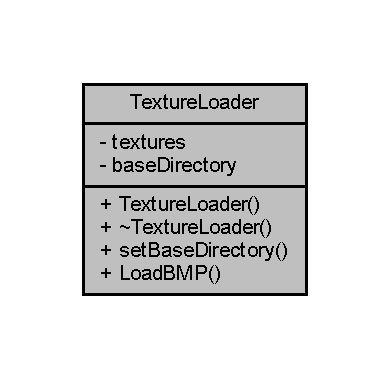
\includegraphics[width=187pt]{class_texture_loader__coll__graph}
\end{center}
\end{figure}
\subsection*{Public Member Functions}
\begin{DoxyCompactItemize}
\item 
\hyperlink{class_texture_loader_aafa6ca3bdbee3874a73aafae39d5c804}{Texture\+Loader} ()
\item 
\hyperlink{class_texture_loader_aee3a49f73e5f88890658b17e9896c4f2}{$\sim$\+Texture\+Loader} ()
\item 
void \hyperlink{class_texture_loader_a08f49a4b5cd9e0d5f84064de749b3eaf}{set\+Base\+Directory} (std\+::string dir)
\item 
int \hyperlink{class_texture_loader_af4f952eca0c705a8ba24ec5a7cb964aa}{Load\+B\+MP} (std\+::string s\+Location, G\+Luint \&texture)
\end{DoxyCompactItemize}
\subsection*{Private Attributes}
\begin{DoxyCompactItemize}
\item 
std\+::vector$<$ \hyperlink{class_texture_loader}{Texture\+Loader} $\ast$ $>$ \hyperlink{class_texture_loader_a09fe47aeb3e99643cae0ebd7ad90a434}{textures}
\item 
std\+::string \hyperlink{class_texture_loader_acd647e9e5e5ca9b1ba8b3e6ef0aa9d84}{base\+Directory}
\end{DoxyCompactItemize}


\subsection{Detailed Description}
This class is used to read models. 

\subsection{Constructor \& Destructor Documentation}
\index{Texture\+Loader@{Texture\+Loader}!Texture\+Loader@{Texture\+Loader}}
\index{Texture\+Loader@{Texture\+Loader}!Texture\+Loader@{Texture\+Loader}}
\subsubsection[{\texorpdfstring{Texture\+Loader()}{TextureLoader()}}]{\setlength{\rightskip}{0pt plus 5cm}Texture\+Loader\+::\+Texture\+Loader (
\begin{DoxyParamCaption}
{}
\end{DoxyParamCaption}
)\hspace{0.3cm}{\ttfamily [inline]}}\hypertarget{class_texture_loader_aafa6ca3bdbee3874a73aafae39d5c804}{}\label{class_texture_loader_aafa6ca3bdbee3874a73aafae39d5c804}
Constructor. \index{Texture\+Loader@{Texture\+Loader}!````~Texture\+Loader@{$\sim$\+Texture\+Loader}}
\index{````~Texture\+Loader@{$\sim$\+Texture\+Loader}!Texture\+Loader@{Texture\+Loader}}
\subsubsection[{\texorpdfstring{$\sim$\+Texture\+Loader()}{~TextureLoader()}}]{\setlength{\rightskip}{0pt plus 5cm}Texture\+Loader\+::$\sim$\+Texture\+Loader (
\begin{DoxyParamCaption}
{}
\end{DoxyParamCaption}
)\hspace{0.3cm}{\ttfamily [inline]}}\hypertarget{class_texture_loader_aee3a49f73e5f88890658b17e9896c4f2}{}\label{class_texture_loader_aee3a49f73e5f88890658b17e9896c4f2}
Desctructor. 

Here is the call graph for this function\+:\nopagebreak
\begin{figure}[H]
\begin{center}
\leavevmode
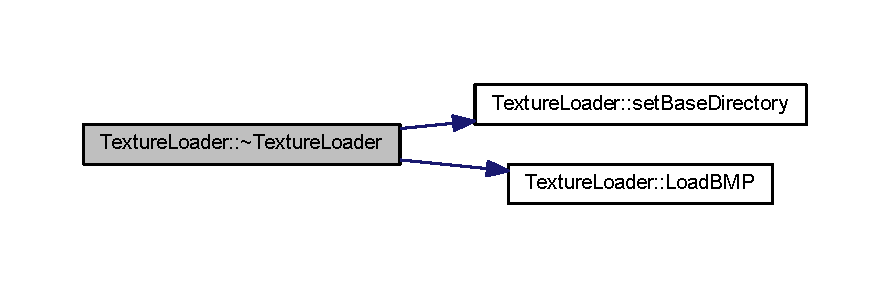
\includegraphics[width=350pt]{class_texture_loader_aee3a49f73e5f88890658b17e9896c4f2_cgraph}
\end{center}
\end{figure}




\subsection{Member Function Documentation}
\index{Texture\+Loader@{Texture\+Loader}!Load\+B\+MP@{Load\+B\+MP}}
\index{Load\+B\+MP@{Load\+B\+MP}!Texture\+Loader@{Texture\+Loader}}
\subsubsection[{\texorpdfstring{Load\+B\+M\+P(std\+::string s\+Location, G\+Luint \&texture)}{LoadBMP(std::string sLocation, GLuint &texture)}}]{\setlength{\rightskip}{0pt plus 5cm}int Texture\+Loader\+::\+Load\+B\+MP (
\begin{DoxyParamCaption}
\item[{std\+::string}]{s\+Location, }
\item[{G\+Luint \&}]{texture}
\end{DoxyParamCaption}
)}\hypertarget{class_texture_loader_af4f952eca0c705a8ba24ec5a7cb964aa}{}\label{class_texture_loader_af4f952eca0c705a8ba24ec5a7cb964aa}
Load B\+MP file. 
\begin{DoxyParams}{Parameters}
{\em s\+Location} & = Location of a file. \\
\hline
{\em \&texture} & = Refrence to the texture. \\
\hline
\end{DoxyParams}
\begin{DoxyReturn}{Returns}
0 = Success code. 
\end{DoxyReturn}
\index{Texture\+Loader@{Texture\+Loader}!set\+Base\+Directory@{set\+Base\+Directory}}
\index{set\+Base\+Directory@{set\+Base\+Directory}!Texture\+Loader@{Texture\+Loader}}
\subsubsection[{\texorpdfstring{set\+Base\+Directory(std\+::string dir)}{setBaseDirectory(std::string dir)}}]{\setlength{\rightskip}{0pt plus 5cm}void Texture\+Loader\+::set\+Base\+Directory (
\begin{DoxyParamCaption}
\item[{std\+::string}]{dir}
\end{DoxyParamCaption}
)}\hypertarget{class_texture_loader_a08f49a4b5cd9e0d5f84064de749b3eaf}{}\label{class_texture_loader_a08f49a4b5cd9e0d5f84064de749b3eaf}
Sets our base directory. 
\begin{DoxyParams}{Parameters}
{\em dir} & = Our base directory. \\
\hline
\end{DoxyParams}


\subsection{Member Data Documentation}
\index{Texture\+Loader@{Texture\+Loader}!base\+Directory@{base\+Directory}}
\index{base\+Directory@{base\+Directory}!Texture\+Loader@{Texture\+Loader}}
\subsubsection[{\texorpdfstring{base\+Directory}{baseDirectory}}]{\setlength{\rightskip}{0pt plus 5cm}std\+::string Texture\+Loader\+::base\+Directory\hspace{0.3cm}{\ttfamily [private]}}\hypertarget{class_texture_loader_acd647e9e5e5ca9b1ba8b3e6ef0aa9d84}{}\label{class_texture_loader_acd647e9e5e5ca9b1ba8b3e6ef0aa9d84}
Our base directory with models. \index{Texture\+Loader@{Texture\+Loader}!textures@{textures}}
\index{textures@{textures}!Texture\+Loader@{Texture\+Loader}}
\subsubsection[{\texorpdfstring{textures}{textures}}]{\setlength{\rightskip}{0pt plus 5cm}std\+::vector$<${\bf Texture\+Loader}$\ast$$>$ Texture\+Loader\+::textures\hspace{0.3cm}{\ttfamily [private]}}\hypertarget{class_texture_loader_a09fe47aeb3e99643cae0ebd7ad90a434}{}\label{class_texture_loader_a09fe47aeb3e99643cae0ebd7ad90a434}
Vector of models. 

The documentation for this class was generated from the following file\+:\begin{DoxyCompactItemize}
\item 
C\+:/\+Airport/include/\hyperlink{texture_loader_8h}{texture\+Loader.\+h}\end{DoxyCompactItemize}

\hypertarget{class_vector_maths}{}\section{Vector\+Maths Class Reference}
\label{class_vector_maths}\index{Vector\+Maths@{Vector\+Maths}}


This class is used to peroform mathematic calculations.  




{\ttfamily \#include $<$vector\+Maths.\+h$>$}



Collaboration diagram for Vector\+Maths\+:\nopagebreak
\begin{figure}[H]
\begin{center}
\leavevmode
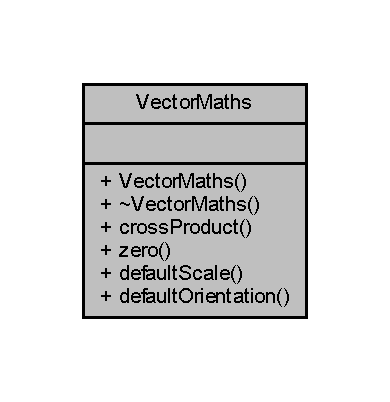
\includegraphics[width=187pt]{class_vector_maths__coll__graph}
\end{center}
\end{figure}
\subsection*{Public Member Functions}
\begin{DoxyCompactItemize}
\item 
\hyperlink{class_vector_maths_af14f2937b1a287972ae741082c63e6e2}{Vector\+Maths} ()
\item 
\hyperlink{class_vector_maths_ad8116f32c0c6a39a688303822f3c4611}{$\sim$\+Vector\+Maths} ()
\item 
sf\+::\+Vector3f \hyperlink{class_vector_maths_afd6cdceae635ef42bf7f638df65d284b}{cross\+Product} (sf\+::\+Vector3f first, sf\+::\+Vector3f second)
\item 
sf\+::\+Vector3f \hyperlink{class_vector_maths_a6ebf2d551c20c0aa08a1d36da3533b21}{zero} ()
\item 
sf\+::\+Vector3f \hyperlink{class_vector_maths_a9dd450c6e51df1eab7dd7824fb10155e}{default\+Scale} ()
\item 
sf\+::\+Vector3f \hyperlink{class_vector_maths_a9fd39cd1a0f66f19b88147cad85f9535}{default\+Orientation} ()
\end{DoxyCompactItemize}


\subsection{Detailed Description}
This class is used to peroform mathematic calculations. 

\subsection{Constructor \& Destructor Documentation}
\index{Vector\+Maths@{Vector\+Maths}!Vector\+Maths@{Vector\+Maths}}
\index{Vector\+Maths@{Vector\+Maths}!Vector\+Maths@{Vector\+Maths}}
\subsubsection[{\texorpdfstring{Vector\+Maths()}{VectorMaths()}}]{\setlength{\rightskip}{0pt plus 5cm}Vector\+Maths\+::\+Vector\+Maths (
\begin{DoxyParamCaption}
{}
\end{DoxyParamCaption}
)\hspace{0.3cm}{\ttfamily [inline]}}\hypertarget{class_vector_maths_af14f2937b1a287972ae741082c63e6e2}{}\label{class_vector_maths_af14f2937b1a287972ae741082c63e6e2}
Constructor. \index{Vector\+Maths@{Vector\+Maths}!````~Vector\+Maths@{$\sim$\+Vector\+Maths}}
\index{````~Vector\+Maths@{$\sim$\+Vector\+Maths}!Vector\+Maths@{Vector\+Maths}}
\subsubsection[{\texorpdfstring{$\sim$\+Vector\+Maths()}{~VectorMaths()}}]{\setlength{\rightskip}{0pt plus 5cm}Vector\+Maths\+::$\sim$\+Vector\+Maths (
\begin{DoxyParamCaption}
{}
\end{DoxyParamCaption}
)\hspace{0.3cm}{\ttfamily [inline]}}\hypertarget{class_vector_maths_ad8116f32c0c6a39a688303822f3c4611}{}\label{class_vector_maths_ad8116f32c0c6a39a688303822f3c4611}


Here is the call graph for this function\+:\nopagebreak
\begin{figure}[H]
\begin{center}
\leavevmode
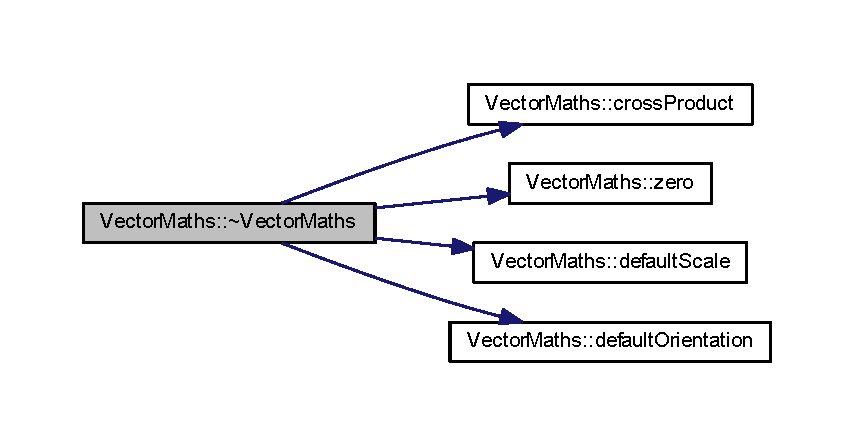
\includegraphics[width=350pt]{class_vector_maths_ad8116f32c0c6a39a688303822f3c4611_cgraph}
\end{center}
\end{figure}




\subsection{Member Function Documentation}
\index{Vector\+Maths@{Vector\+Maths}!cross\+Product@{cross\+Product}}
\index{cross\+Product@{cross\+Product}!Vector\+Maths@{Vector\+Maths}}
\subsubsection[{\texorpdfstring{cross\+Product(sf\+::\+Vector3f first, sf\+::\+Vector3f second)}{crossProduct(sf::Vector3f first, sf::Vector3f second)}}]{\setlength{\rightskip}{0pt plus 5cm}sf\+::\+Vector3f Vector\+Maths\+::cross\+Product (
\begin{DoxyParamCaption}
\item[{sf\+::\+Vector3f}]{first, }
\item[{sf\+::\+Vector3f}]{second}
\end{DoxyParamCaption}
)}\hypertarget{class_vector_maths_afd6cdceae635ef42bf7f638df65d284b}{}\label{class_vector_maths_afd6cdceae635ef42bf7f638df65d284b}

\begin{DoxyParams}{Parameters}
{\em first} & = First vector. \\
\hline
{\em second} & = Second vector. \\
\hline
\end{DoxyParams}
\index{Vector\+Maths@{Vector\+Maths}!default\+Orientation@{default\+Orientation}}
\index{default\+Orientation@{default\+Orientation}!Vector\+Maths@{Vector\+Maths}}
\subsubsection[{\texorpdfstring{default\+Orientation()}{defaultOrientation()}}]{\setlength{\rightskip}{0pt plus 5cm}sf\+::\+Vector3f Vector\+Maths\+::default\+Orientation (
\begin{DoxyParamCaption}
{}
\end{DoxyParamCaption}
)}\hypertarget{class_vector_maths_a9fd39cd1a0f66f19b88147cad85f9535}{}\label{class_vector_maths_a9fd39cd1a0f66f19b88147cad85f9535}
\begin{DoxyReturn}{Returns}
orientation = Default orientation such as 0, 0, 0. 
\end{DoxyReturn}
\index{Vector\+Maths@{Vector\+Maths}!default\+Scale@{default\+Scale}}
\index{default\+Scale@{default\+Scale}!Vector\+Maths@{Vector\+Maths}}
\subsubsection[{\texorpdfstring{default\+Scale()}{defaultScale()}}]{\setlength{\rightskip}{0pt plus 5cm}sf\+::\+Vector3f Vector\+Maths\+::default\+Scale (
\begin{DoxyParamCaption}
{}
\end{DoxyParamCaption}
)}\hypertarget{class_vector_maths_a9dd450c6e51df1eab7dd7824fb10155e}{}\label{class_vector_maths_a9dd450c6e51df1eab7dd7824fb10155e}
\begin{DoxyReturn}{Returns}
scale = default scale such as 1, 1, 1. 
\end{DoxyReturn}
\index{Vector\+Maths@{Vector\+Maths}!zero@{zero}}
\index{zero@{zero}!Vector\+Maths@{Vector\+Maths}}
\subsubsection[{\texorpdfstring{zero()}{zero()}}]{\setlength{\rightskip}{0pt plus 5cm}sf\+::\+Vector3f Vector\+Maths\+::zero (
\begin{DoxyParamCaption}
{}
\end{DoxyParamCaption}
)}\hypertarget{class_vector_maths_a6ebf2d551c20c0aa08a1d36da3533b21}{}\label{class_vector_maths_a6ebf2d551c20c0aa08a1d36da3533b21}
\begin{DoxyReturn}{Returns}
zero = empty vector such as 0, 0, 0. 
\end{DoxyReturn}


The documentation for this class was generated from the following file\+:\begin{DoxyCompactItemize}
\item 
C\+:/\+Airport/include/\hyperlink{vector_maths_8h}{vector\+Maths.\+h}\end{DoxyCompactItemize}

\chapter{File Documentation}
\hypertarget{camera_8h}{}\section{C\+:/\+Airport/include/camera.h File Reference}
\label{camera_8h}\index{C\+:/\+Airport/include/camera.\+h@{C\+:/\+Airport/include/camera.\+h}}
{\ttfamily \#include \char`\"{}headers.\+h\char`\"{}}\\*
Include dependency graph for camera.\+h\+:\nopagebreak
\begin{figure}[H]
\begin{center}
\leavevmode
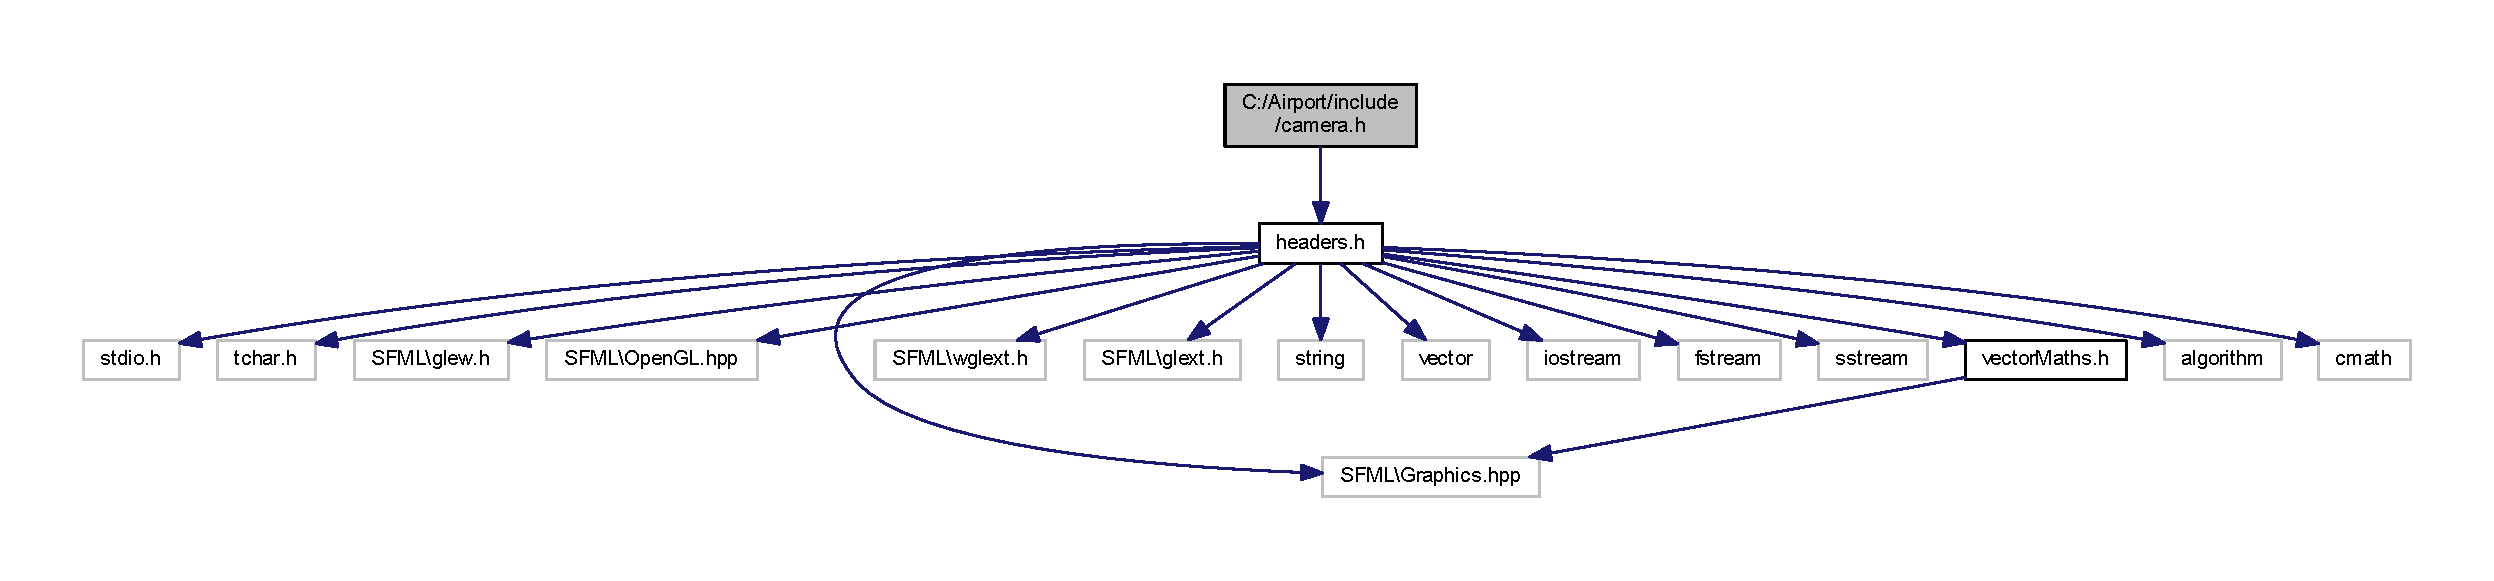
\includegraphics[width=350pt]{camera_8h__incl}
\end{center}
\end{figure}
This graph shows which files directly or indirectly include this file\+:\nopagebreak
\begin{figure}[H]
\begin{center}
\leavevmode
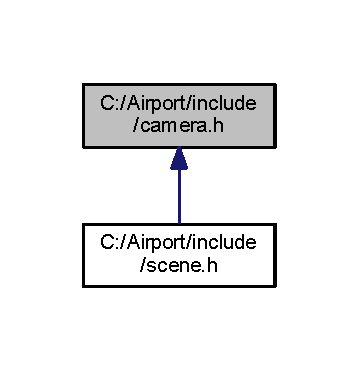
\includegraphics[width=172pt]{camera_8h__dep__incl}
\end{center}
\end{figure}
\subsection*{Classes}
\begin{DoxyCompactItemize}
\item 
class \hyperlink{class_camera}{Camera}
\begin{DoxyCompactList}\small\item\em This class is used to create a camera. \end{DoxyCompactList}\end{DoxyCompactItemize}

\hypertarget{headers_8h}{}\section{C\+:/\+Airport/include/headers.h File Reference}
\label{headers_8h}\index{C\+:/\+Airport/include/headers.\+h@{C\+:/\+Airport/include/headers.\+h}}
{\ttfamily \#include $<$stdio.\+h$>$}\\*
{\ttfamily \#include $<$tchar.\+h$>$}\\*
{\ttfamily \#include $<$S\+F\+M\+L\textbackslash{}glew.\+h$>$}\\*
{\ttfamily \#include $<$S\+F\+M\+L\textbackslash{}\+Open\+G\+L.\+hpp$>$}\\*
{\ttfamily \#include $<$S\+F\+M\+L\textbackslash{}\+Graphics.\+hpp$>$}\\*
{\ttfamily \#include $<$S\+F\+M\+L\textbackslash{}wglext.\+h$>$}\\*
{\ttfamily \#include $<$S\+F\+M\+L\textbackslash{}glext.\+h$>$}\\*
{\ttfamily \#include $<$string$>$}\\*
{\ttfamily \#include $<$vector$>$}\\*
{\ttfamily \#include $<$iostream$>$}\\*
{\ttfamily \#include $<$fstream$>$}\\*
{\ttfamily \#include $<$sstream$>$}\\*
{\ttfamily \#include \char`\"{}vector\+Maths.\+h\char`\"{}}\\*
{\ttfamily \#include $<$algorithm$>$}\\*
{\ttfamily \#include $<$cmath$>$}\\*
Include dependency graph for headers.\+h\+:\nopagebreak
\begin{figure}[H]
\begin{center}
\leavevmode
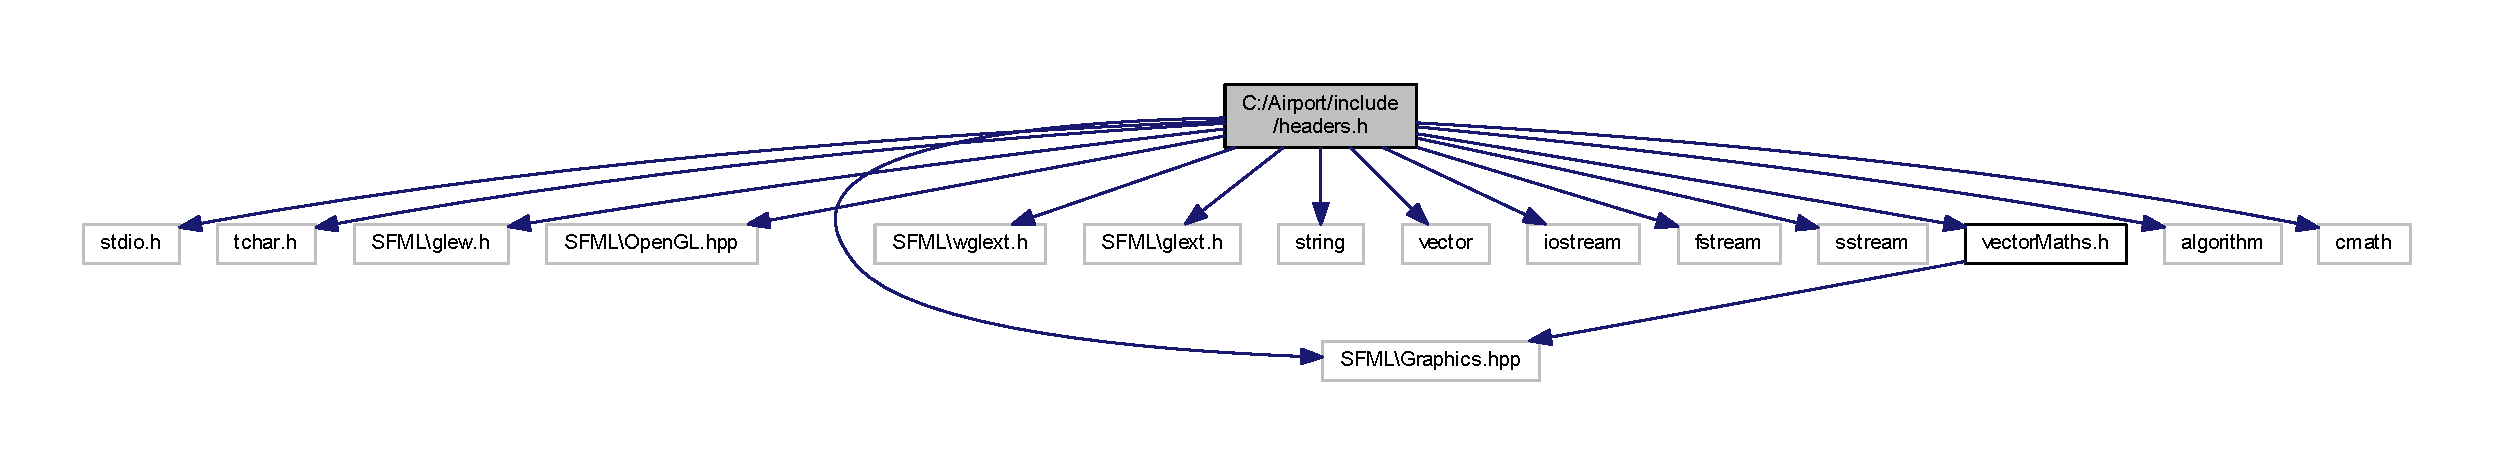
\includegraphics[width=350pt]{headers_8h__incl}
\end{center}
\end{figure}
This graph shows which files directly or indirectly include this file\+:\nopagebreak
\begin{figure}[H]
\begin{center}
\leavevmode
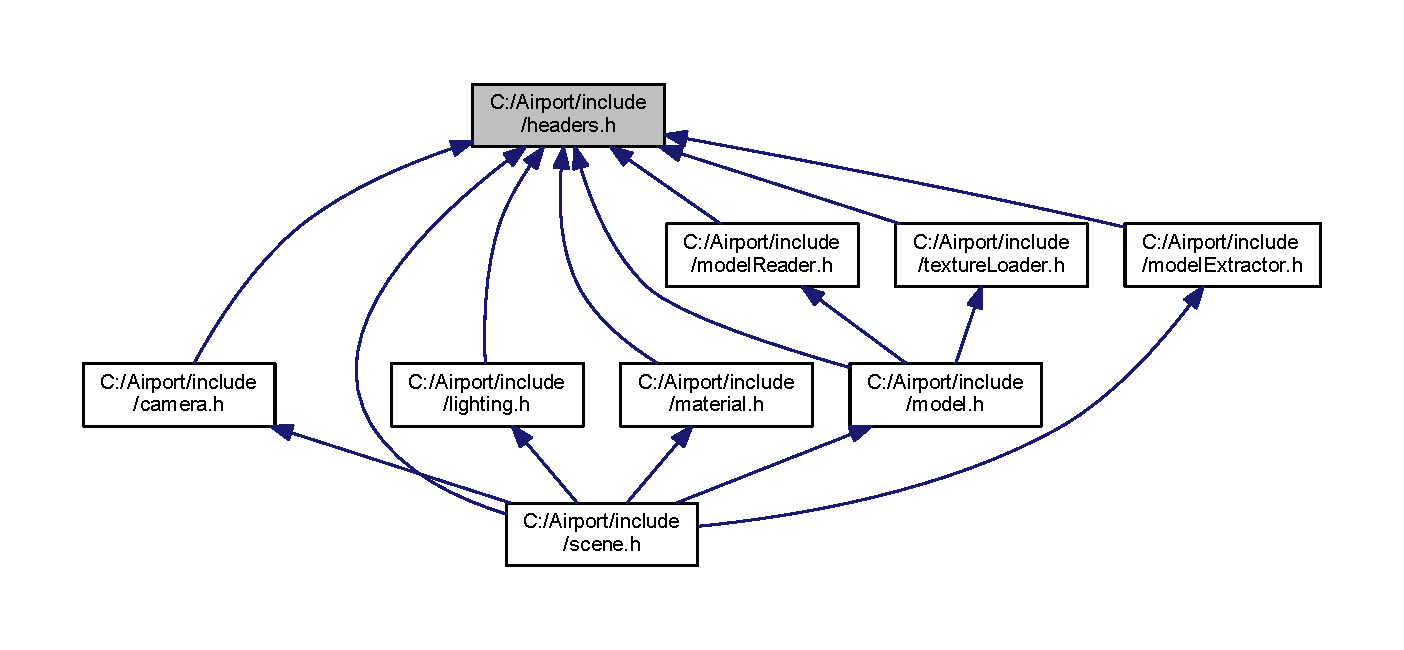
\includegraphics[width=350pt]{headers_8h__dep__incl}
\end{center}
\end{figure}
\subsection*{Macros}
\begin{DoxyCompactItemize}
\item 
\#define \hyperlink{headers_8h_a120fb070bddb21f0bd899f50252c4cb5}{G\+L\+\_\+\+G\+L\+E\+X\+T\+\_\+\+P\+R\+O\+T\+O\+T\+Y\+P\+ES}~1
\item 
\#define \hyperlink{headers_8h_abcde84ea0ef5f934384e4620f092c85a}{G\+L\+E\+W\+\_\+\+S\+T\+A\+T\+IC}
\item 
\#define \hyperlink{headers_8h_a525335710b53cb064ca56b936120431e}{\+\_\+\+U\+S\+E\+\_\+\+M\+A\+T\+H\+\_\+\+D\+E\+F\+I\+N\+ES}
\end{DoxyCompactItemize}


\subsection{Macro Definition Documentation}
\index{headers.\+h@{headers.\+h}!\+\_\+\+U\+S\+E\+\_\+\+M\+A\+T\+H\+\_\+\+D\+E\+F\+I\+N\+ES@{\+\_\+\+U\+S\+E\+\_\+\+M\+A\+T\+H\+\_\+\+D\+E\+F\+I\+N\+ES}}
\index{\+\_\+\+U\+S\+E\+\_\+\+M\+A\+T\+H\+\_\+\+D\+E\+F\+I\+N\+ES@{\+\_\+\+U\+S\+E\+\_\+\+M\+A\+T\+H\+\_\+\+D\+E\+F\+I\+N\+ES}!headers.\+h@{headers.\+h}}
\subsubsection[{\texorpdfstring{\+\_\+\+U\+S\+E\+\_\+\+M\+A\+T\+H\+\_\+\+D\+E\+F\+I\+N\+ES}{_USE_MATH_DEFINES}}]{\setlength{\rightskip}{0pt plus 5cm}\#define \+\_\+\+U\+S\+E\+\_\+\+M\+A\+T\+H\+\_\+\+D\+E\+F\+I\+N\+ES}\hypertarget{headers_8h_a525335710b53cb064ca56b936120431e}{}\label{headers_8h_a525335710b53cb064ca56b936120431e}
\index{headers.\+h@{headers.\+h}!G\+L\+\_\+\+G\+L\+E\+X\+T\+\_\+\+P\+R\+O\+T\+O\+T\+Y\+P\+ES@{G\+L\+\_\+\+G\+L\+E\+X\+T\+\_\+\+P\+R\+O\+T\+O\+T\+Y\+P\+ES}}
\index{G\+L\+\_\+\+G\+L\+E\+X\+T\+\_\+\+P\+R\+O\+T\+O\+T\+Y\+P\+ES@{G\+L\+\_\+\+G\+L\+E\+X\+T\+\_\+\+P\+R\+O\+T\+O\+T\+Y\+P\+ES}!headers.\+h@{headers.\+h}}
\subsubsection[{\texorpdfstring{G\+L\+\_\+\+G\+L\+E\+X\+T\+\_\+\+P\+R\+O\+T\+O\+T\+Y\+P\+ES}{GL_GLEXT_PROTOTYPES}}]{\setlength{\rightskip}{0pt plus 5cm}\#define G\+L\+\_\+\+G\+L\+E\+X\+T\+\_\+\+P\+R\+O\+T\+O\+T\+Y\+P\+ES~1}\hypertarget{headers_8h_a120fb070bddb21f0bd899f50252c4cb5}{}\label{headers_8h_a120fb070bddb21f0bd899f50252c4cb5}
\index{headers.\+h@{headers.\+h}!G\+L\+E\+W\+\_\+\+S\+T\+A\+T\+IC@{G\+L\+E\+W\+\_\+\+S\+T\+A\+T\+IC}}
\index{G\+L\+E\+W\+\_\+\+S\+T\+A\+T\+IC@{G\+L\+E\+W\+\_\+\+S\+T\+A\+T\+IC}!headers.\+h@{headers.\+h}}
\subsubsection[{\texorpdfstring{G\+L\+E\+W\+\_\+\+S\+T\+A\+T\+IC}{GLEW_STATIC}}]{\setlength{\rightskip}{0pt plus 5cm}\#define G\+L\+E\+W\+\_\+\+S\+T\+A\+T\+IC}\hypertarget{headers_8h_abcde84ea0ef5f934384e4620f092c85a}{}\label{headers_8h_abcde84ea0ef5f934384e4620f092c85a}

\hypertarget{lighting_8h}{}\section{C\+:/\+Airport/include/lighting.h File Reference}
\label{lighting_8h}\index{C\+:/\+Airport/include/lighting.\+h@{C\+:/\+Airport/include/lighting.\+h}}
{\ttfamily \#include $<$headers.\+h$>$}\\*
{\ttfamily \#include $<$array$>$}\\*
Include dependency graph for lighting.\+h\+:\nopagebreak
\begin{figure}[H]
\begin{center}
\leavevmode
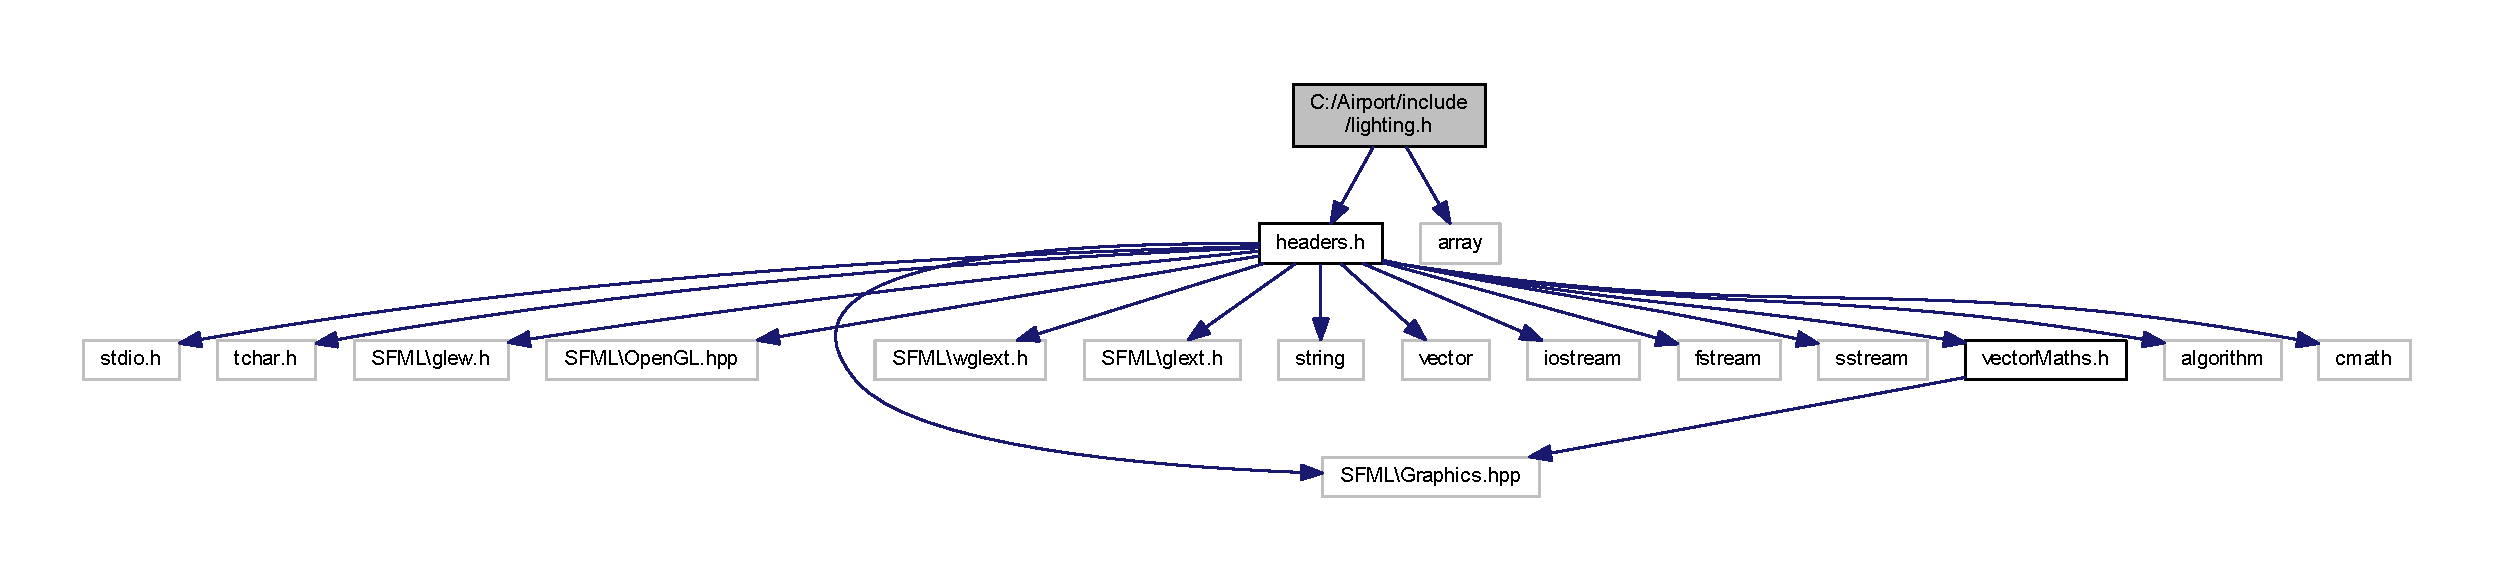
\includegraphics[width=350pt]{lighting_8h__incl}
\end{center}
\end{figure}
This graph shows which files directly or indirectly include this file\+:\nopagebreak
\begin{figure}[H]
\begin{center}
\leavevmode
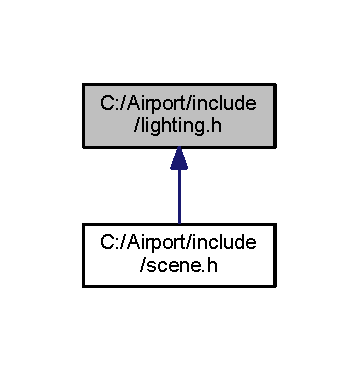
\includegraphics[width=172pt]{lighting_8h__dep__incl}
\end{center}
\end{figure}
\subsection*{Classes}
\begin{DoxyCompactItemize}
\item 
class \hyperlink{class_lighting}{Lighting}
\begin{DoxyCompactList}\small\item\em This class is used to create a lighting. \end{DoxyCompactList}\end{DoxyCompactItemize}

\hypertarget{material_8h}{}\section{C\+:/\+Airport/include/material.h File Reference}
\label{material_8h}\index{C\+:/\+Airport/include/material.\+h@{C\+:/\+Airport/include/material.\+h}}
{\ttfamily \#include \char`\"{}headers.\+h\char`\"{}}\\*
Include dependency graph for material.\+h\+:\nopagebreak
\begin{figure}[H]
\begin{center}
\leavevmode
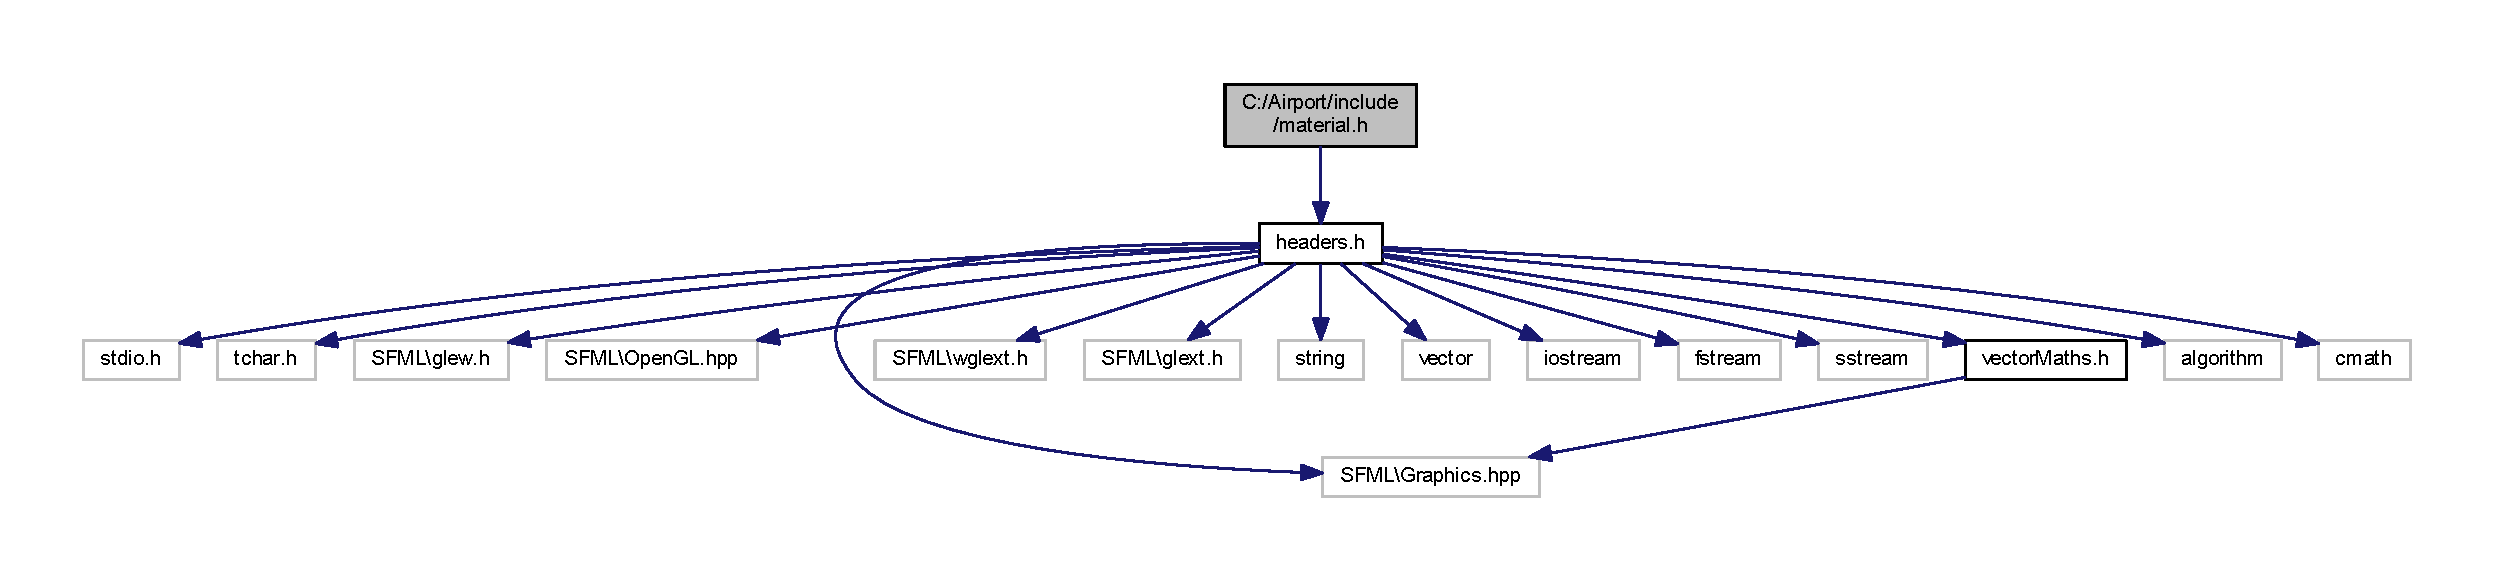
\includegraphics[width=350pt]{material_8h__incl}
\end{center}
\end{figure}
This graph shows which files directly or indirectly include this file\+:\nopagebreak
\begin{figure}[H]
\begin{center}
\leavevmode
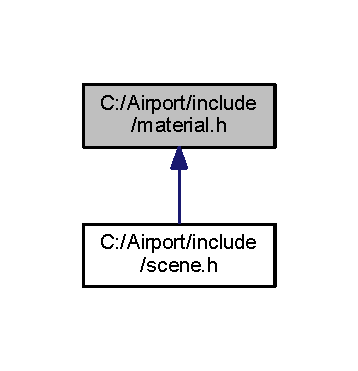
\includegraphics[width=172pt]{material_8h__dep__incl}
\end{center}
\end{figure}
\subsection*{Classes}
\begin{DoxyCompactItemize}
\item 
class \hyperlink{class_material}{Material}
\begin{DoxyCompactList}\small\item\em This class is used to create a material. \end{DoxyCompactList}\end{DoxyCompactItemize}

\hypertarget{model_8h}{}\section{C\+:/\+Airport/include/model.h File Reference}
\label{model_8h}\index{C\+:/\+Airport/include/model.\+h@{C\+:/\+Airport/include/model.\+h}}
{\ttfamily \#include \char`\"{}headers.\+h\char`\"{}}\\*
{\ttfamily \#include \char`\"{}model\+Reader.\+h\char`\"{}}\\*
{\ttfamily \#include \char`\"{}texture\+Loader.\+h\char`\"{}}\\*
Include dependency graph for model.\+h\+:\nopagebreak
\begin{figure}[H]
\begin{center}
\leavevmode
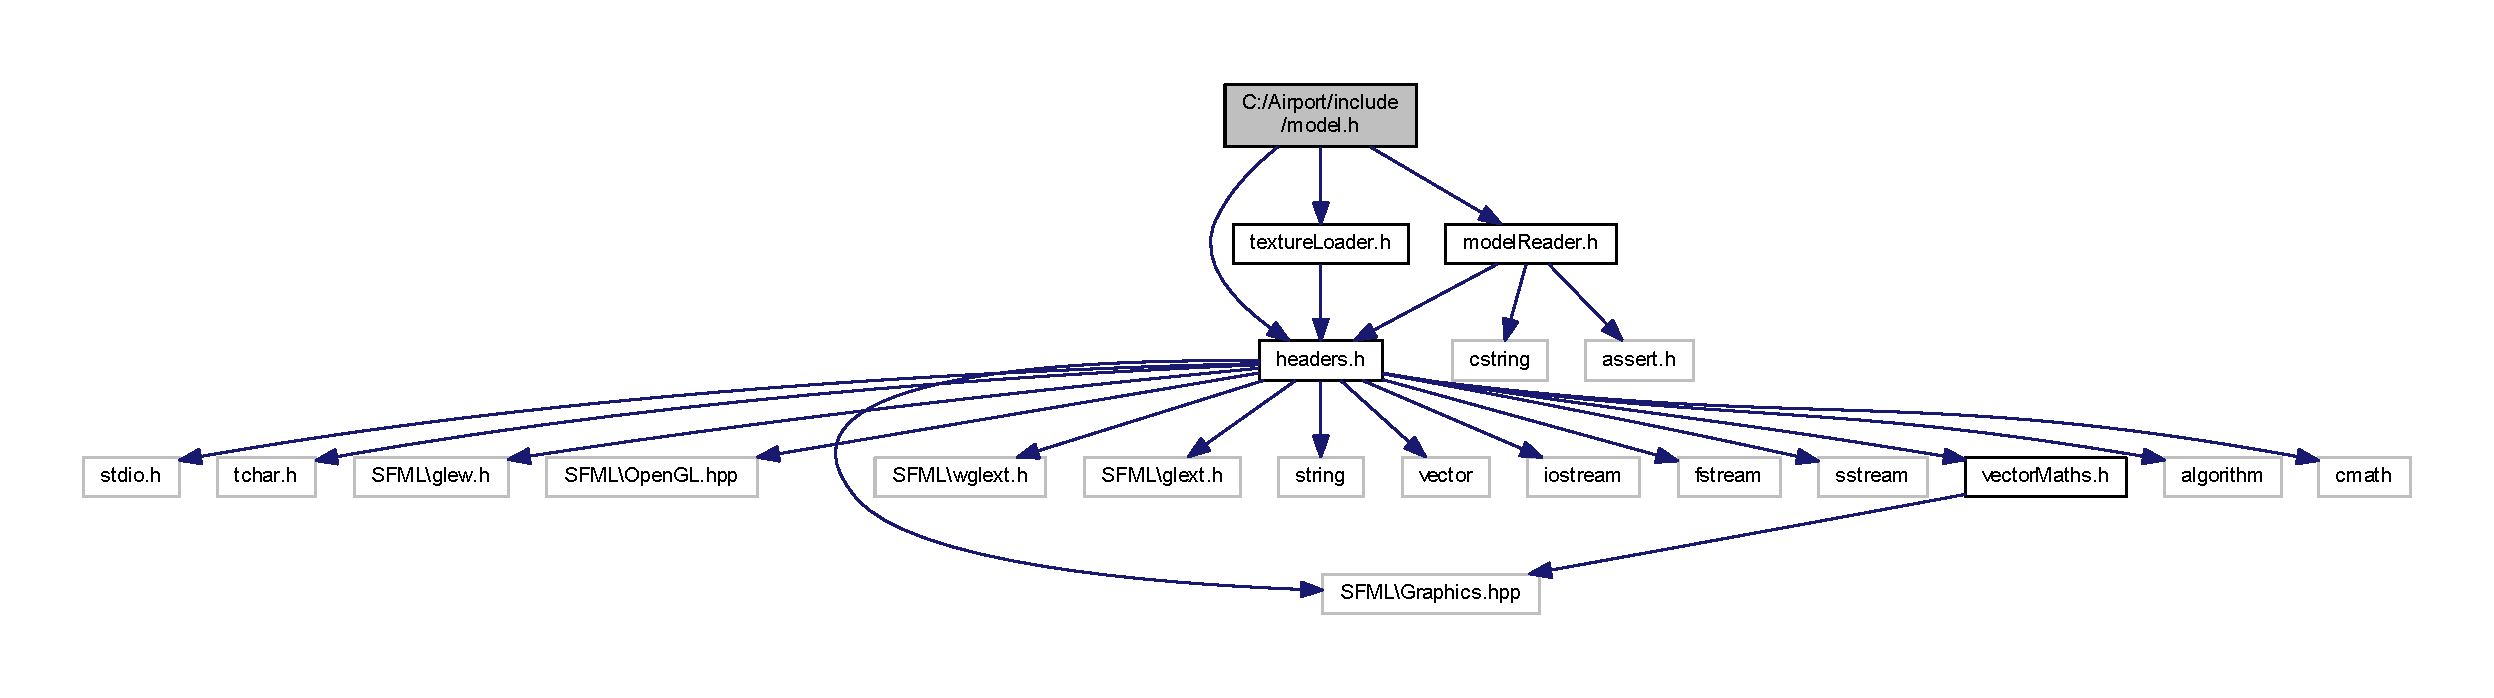
\includegraphics[width=350pt]{model_8h__incl}
\end{center}
\end{figure}
This graph shows which files directly or indirectly include this file\+:\nopagebreak
\begin{figure}[H]
\begin{center}
\leavevmode
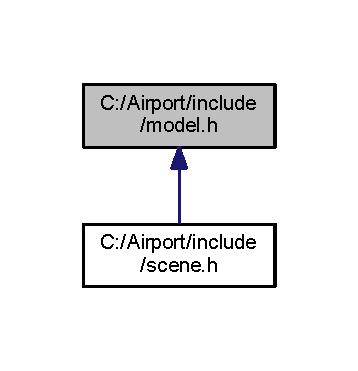
\includegraphics[width=172pt]{model_8h__dep__incl}
\end{center}
\end{figure}
\subsection*{Classes}
\begin{DoxyCompactItemize}
\item 
class \hyperlink{class_model}{Model}
\begin{DoxyCompactList}\small\item\em This class is used to create a model. \end{DoxyCompactList}\end{DoxyCompactItemize}

\hypertarget{model_extractor_8h}{}\section{C\+:/\+Airport/include/model\+Extractor.h File Reference}
\label{model_extractor_8h}\index{C\+:/\+Airport/include/model\+Extractor.\+h@{C\+:/\+Airport/include/model\+Extractor.\+h}}
{\ttfamily \#include \char`\"{}headers.\+h\char`\"{}}\\*
Include dependency graph for model\+Extractor.\+h\+:\nopagebreak
\begin{figure}[H]
\begin{center}
\leavevmode
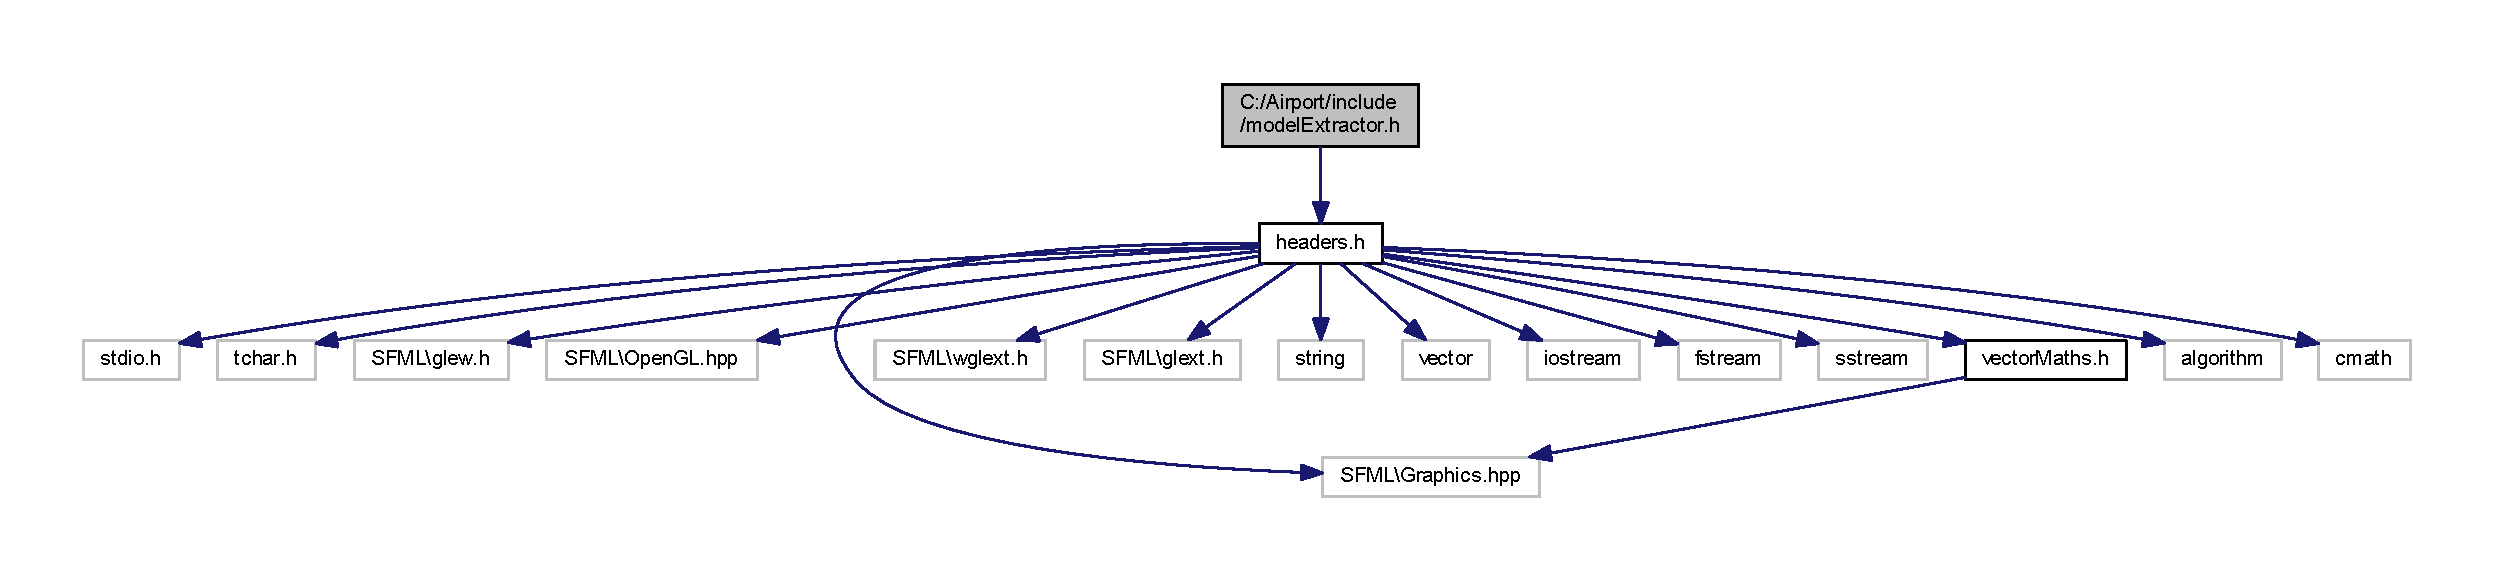
\includegraphics[width=350pt]{model_extractor_8h__incl}
\end{center}
\end{figure}
This graph shows which files directly or indirectly include this file\+:\nopagebreak
\begin{figure}[H]
\begin{center}
\leavevmode
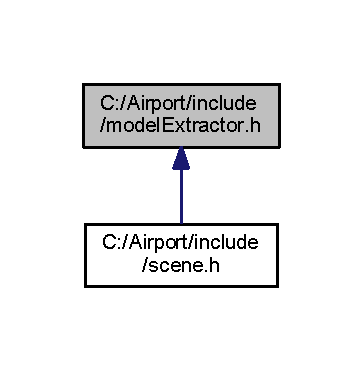
\includegraphics[width=174pt]{model_extractor_8h__dep__incl}
\end{center}
\end{figure}
\subsection*{Classes}
\begin{DoxyCompactItemize}
\item 
class \hyperlink{class_model_extractor}{Model\+Extractor}
\begin{DoxyCompactList}\small\item\em This class is used to extract information about the model from a file. \end{DoxyCompactList}\end{DoxyCompactItemize}

\hypertarget{model_reader_8h}{}\section{C\+:/\+Airport/include/model\+Reader.h File Reference}
\label{model_reader_8h}\index{C\+:/\+Airport/include/model\+Reader.\+h@{C\+:/\+Airport/include/model\+Reader.\+h}}
{\ttfamily \#include $<$cstring$>$}\\*
{\ttfamily \#include $<$assert.\+h$>$}\\*
{\ttfamily \#include $<$headers.\+h$>$}\\*
Include dependency graph for model\+Reader.\+h\+:\nopagebreak
\begin{figure}[H]
\begin{center}
\leavevmode
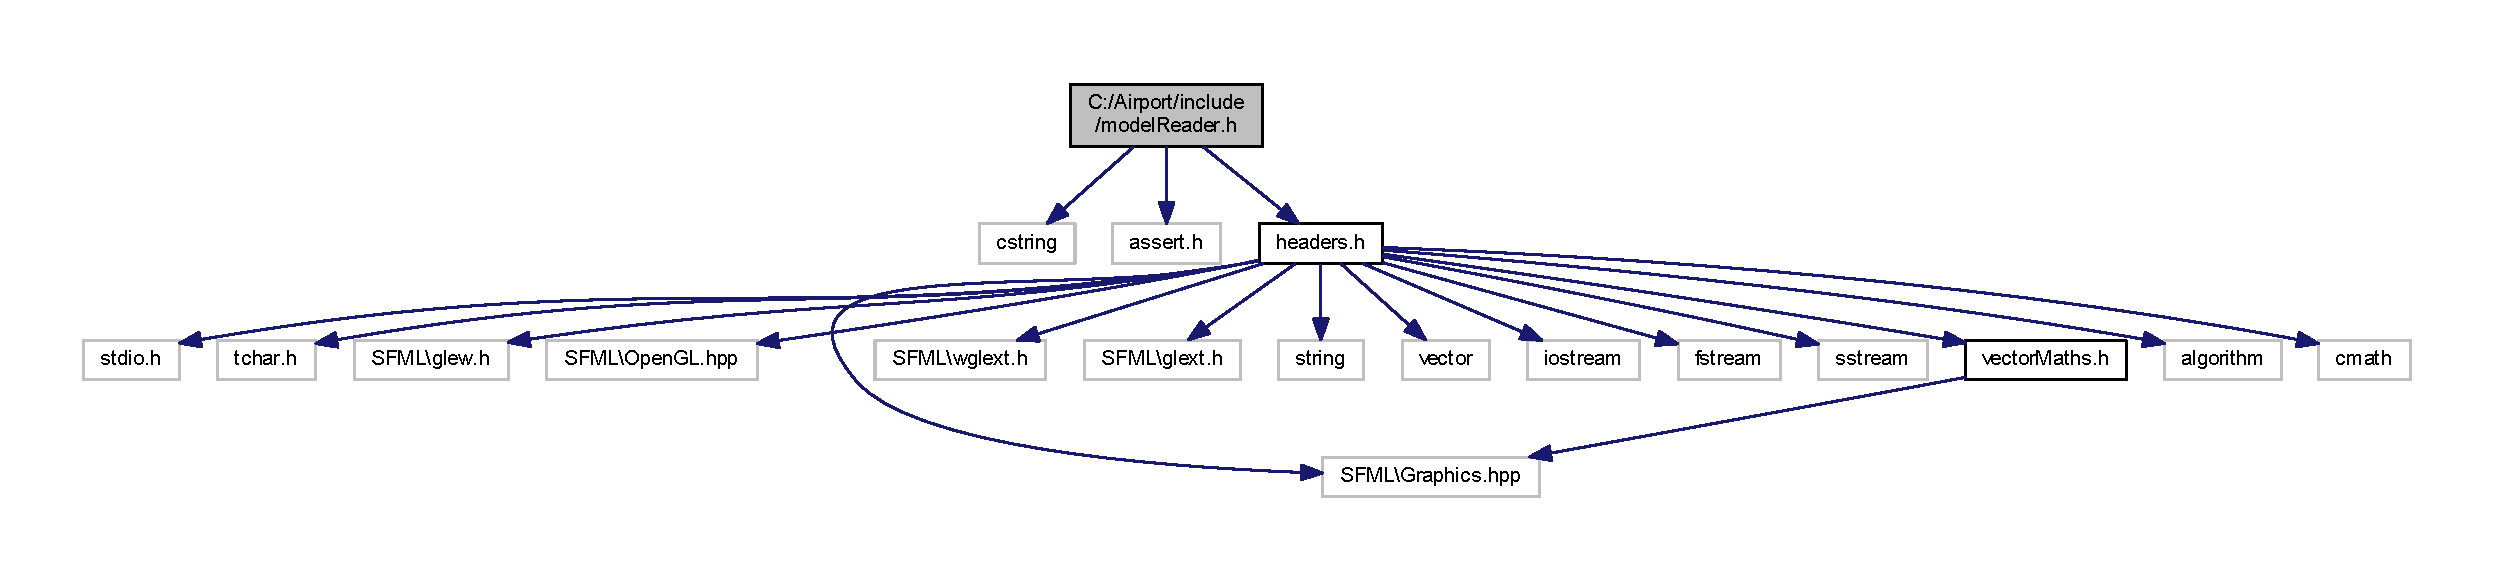
\includegraphics[width=350pt]{model_reader_8h__incl}
\end{center}
\end{figure}
This graph shows which files directly or indirectly include this file\+:\nopagebreak
\begin{figure}[H]
\begin{center}
\leavevmode
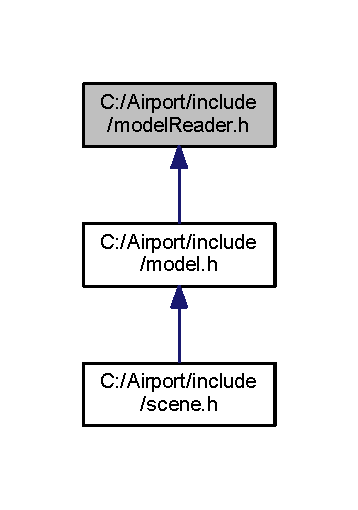
\includegraphics[width=172pt]{model_reader_8h__dep__incl}
\end{center}
\end{figure}
\subsection*{Classes}
\begin{DoxyCompactItemize}
\item 
class \hyperlink{class_model_reader}{Model\+Reader}
\begin{DoxyCompactList}\small\item\em This class is used to read models. \end{DoxyCompactList}\end{DoxyCompactItemize}

\hypertarget{scene_8h}{}\section{C\+:/\+Airport/include/scene.h File Reference}
\label{scene_8h}\index{C\+:/\+Airport/include/scene.\+h@{C\+:/\+Airport/include/scene.\+h}}
{\ttfamily \#include \char`\"{}headers.\+h\char`\"{}}\\*
{\ttfamily \#include \char`\"{}model.\+h\char`\"{}}\\*
{\ttfamily \#include \char`\"{}camera.\+h\char`\"{}}\\*
{\ttfamily \#include \char`\"{}lighting.\+h\char`\"{}}\\*
{\ttfamily \#include $<$array$>$}\\*
{\ttfamily \#include \char`\"{}model\+Extractor.\+h\char`\"{}}\\*
{\ttfamily \#include \char`\"{}material.\+h\char`\"{}}\\*
Include dependency graph for scene.\+h\+:\nopagebreak
\begin{figure}[H]
\begin{center}
\leavevmode
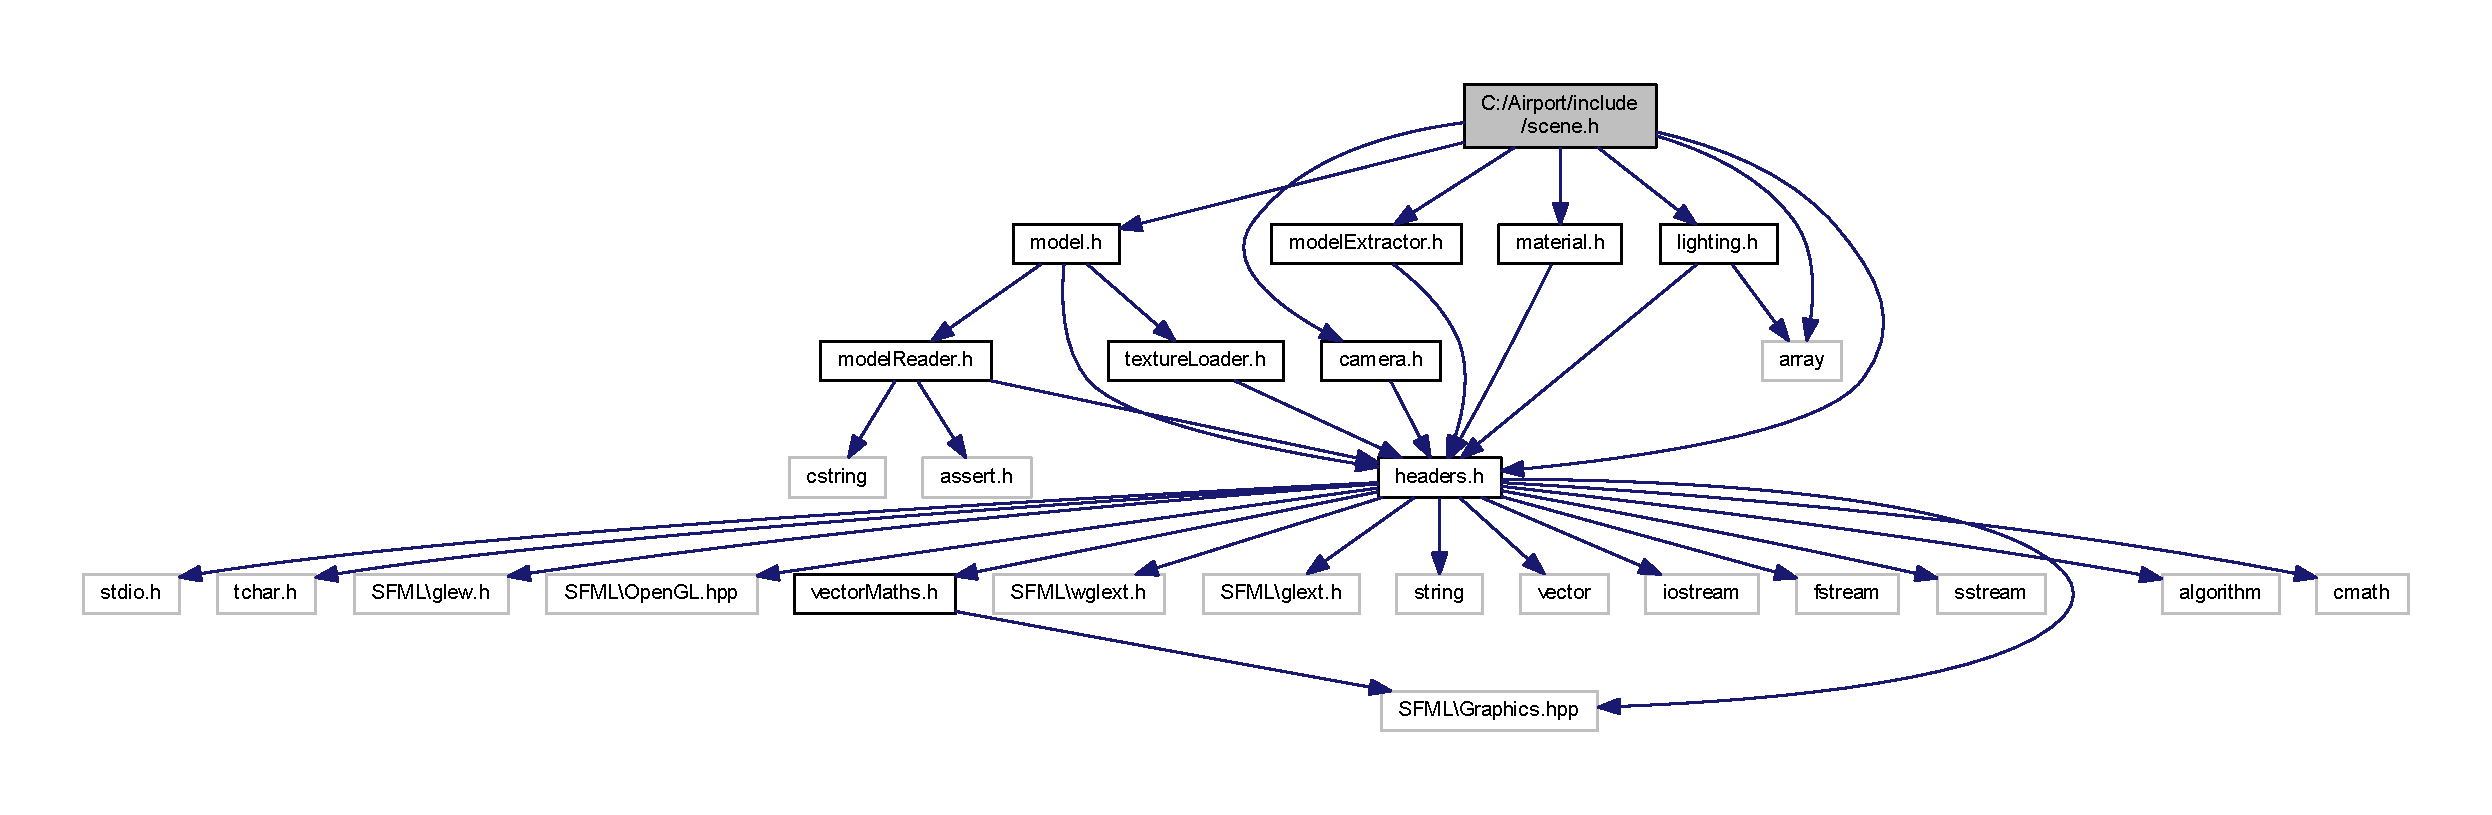
\includegraphics[width=350pt]{scene_8h__incl}
\end{center}
\end{figure}
\subsection*{Classes}
\begin{DoxyCompactItemize}
\item 
class \hyperlink{class_scene}{Scene}
\begin{DoxyCompactList}\small\item\em This class is used to render a scene. \end{DoxyCompactList}\end{DoxyCompactItemize}

\hypertarget{texture_loader_8h}{}\section{C\+:/\+Airport/include/texture\+Loader.h File Reference}
\label{texture_loader_8h}\index{C\+:/\+Airport/include/texture\+Loader.\+h@{C\+:/\+Airport/include/texture\+Loader.\+h}}
{\ttfamily \#include \char`\"{}headers.\+h\char`\"{}}\\*
Include dependency graph for texture\+Loader.\+h\+:\nopagebreak
\begin{figure}[H]
\begin{center}
\leavevmode
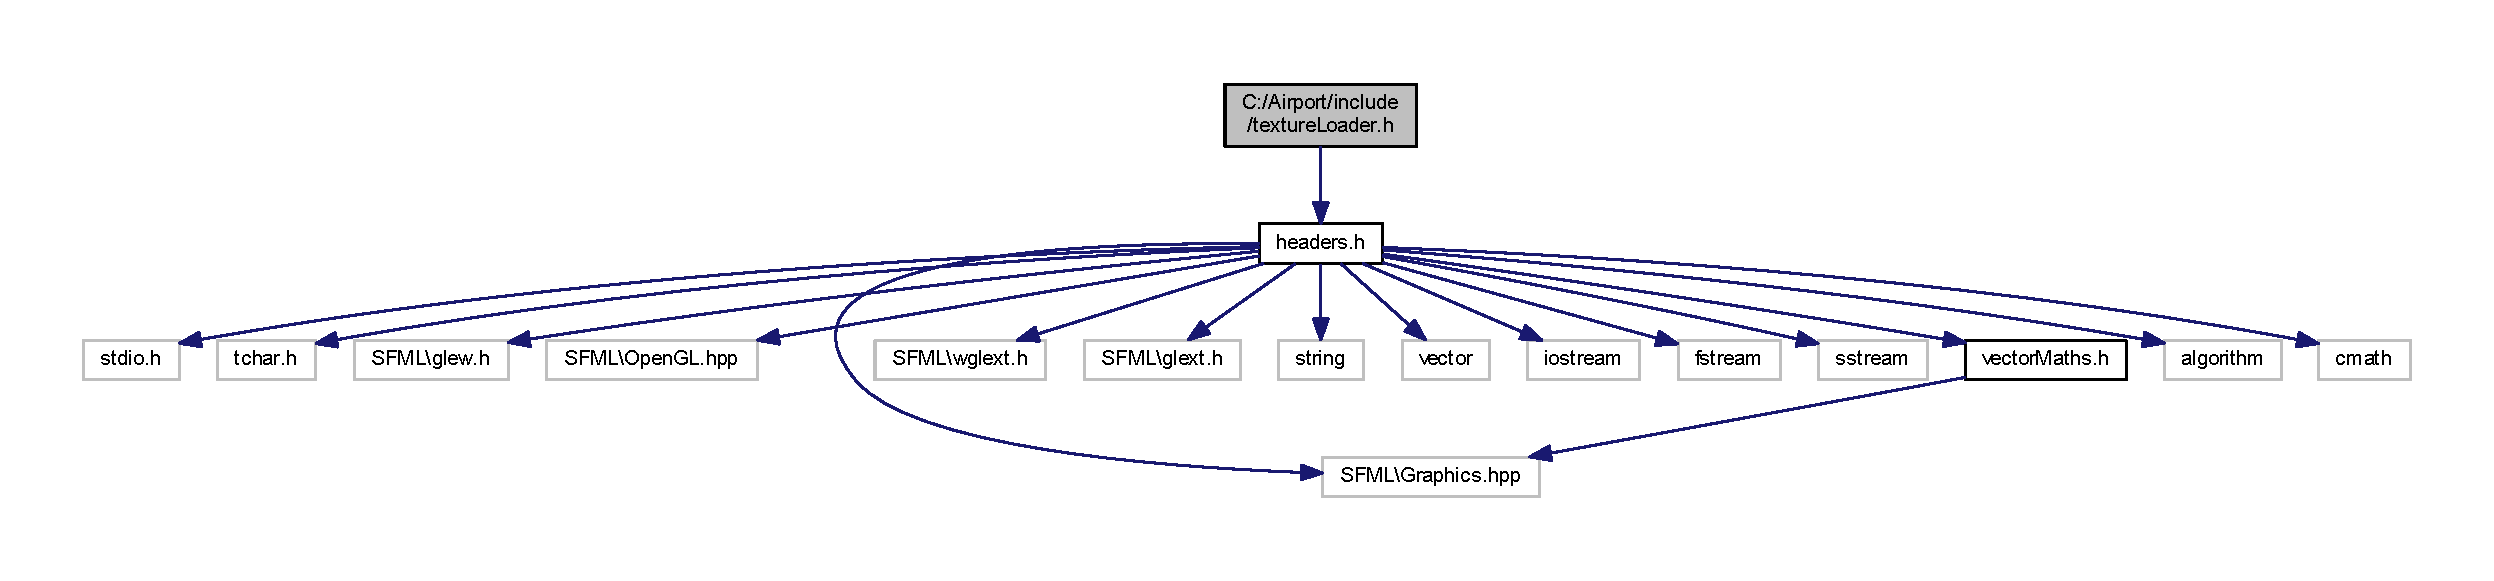
\includegraphics[width=350pt]{texture_loader_8h__incl}
\end{center}
\end{figure}
This graph shows which files directly or indirectly include this file\+:\nopagebreak
\begin{figure}[H]
\begin{center}
\leavevmode
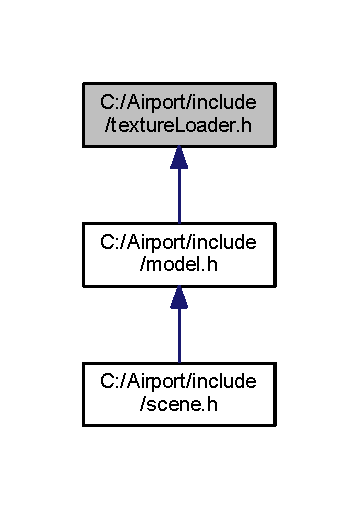
\includegraphics[width=172pt]{texture_loader_8h__dep__incl}
\end{center}
\end{figure}
\subsection*{Classes}
\begin{DoxyCompactItemize}
\item 
class \hyperlink{class_texture_loader}{Texture\+Loader}
\begin{DoxyCompactList}\small\item\em This class is used to read models. \end{DoxyCompactList}\end{DoxyCompactItemize}

\hypertarget{vector_maths_8h}{}\section{C\+:/\+Airport/include/vector\+Maths.h File Reference}
\label{vector_maths_8h}\index{C\+:/\+Airport/include/vector\+Maths.\+h@{C\+:/\+Airport/include/vector\+Maths.\+h}}
{\ttfamily \#include $<$S\+F\+M\+L\textbackslash{}\+Graphics.\+hpp$>$}\\*
Include dependency graph for vector\+Maths.\+h\+:\nopagebreak
\begin{figure}[H]
\begin{center}
\leavevmode
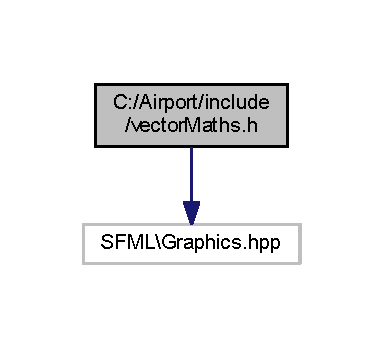
\includegraphics[width=184pt]{vector_maths_8h__incl}
\end{center}
\end{figure}
This graph shows which files directly or indirectly include this file\+:\nopagebreak
\begin{figure}[H]
\begin{center}
\leavevmode
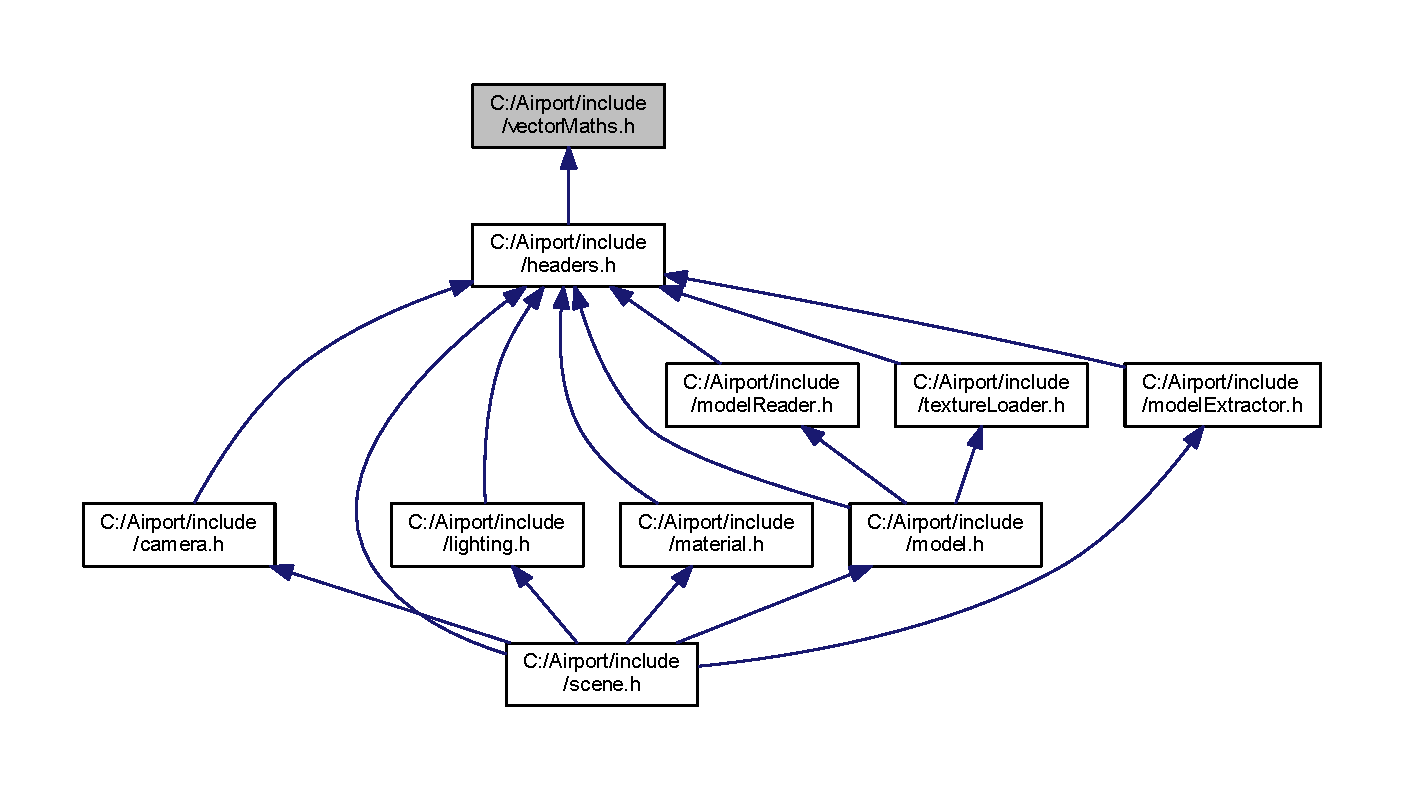
\includegraphics[width=350pt]{vector_maths_8h__dep__incl}
\end{center}
\end{figure}
\subsection*{Classes}
\begin{DoxyCompactItemize}
\item 
class \hyperlink{class_vector_maths}{Vector\+Maths}
\begin{DoxyCompactList}\small\item\em This class is used to peroform mathematic calculations. \end{DoxyCompactList}\end{DoxyCompactItemize}

%--- End generated contents ---

% Index
\backmatter
\newpage
\phantomsection
\clearemptydoublepage
\addcontentsline{toc}{chapter}{Index}
\printindex

\end{document}
